% Options for packages loaded elsewhere
\PassOptionsToPackage{unicode}{hyperref}
\PassOptionsToPackage{hyphens}{url}
\PassOptionsToPackage{dvipsnames,svgnames,x11names}{xcolor}
%
\documentclass[
  10pt,
  dvipsnames,enabledeprecatedfontcommands]{scrartcl}
\title{Bayesian analysis of the NESTA study of interventions against
verbal aggression online}
\author{Rafal Urbaniak}
\date{}

\usepackage{amsmath,amssymb}
\usepackage{lmodern}
\usepackage{iftex}
\ifPDFTeX
  \usepackage[T1]{fontenc}
  \usepackage[utf8]{inputenc}
  \usepackage{textcomp} % provide euro and other symbols
\else % if luatex or xetex
  \usepackage{unicode-math}
  \defaultfontfeatures{Scale=MatchLowercase}
  \defaultfontfeatures[\rmfamily]{Ligatures=TeX,Scale=1}
\fi
% Use upquote if available, for straight quotes in verbatim environments
\IfFileExists{upquote.sty}{\usepackage{upquote}}{}
\IfFileExists{microtype.sty}{% use microtype if available
  \usepackage[]{microtype}
  \UseMicrotypeSet[protrusion]{basicmath} % disable protrusion for tt fonts
}{}
\makeatletter
\@ifundefined{KOMAClassName}{% if non-KOMA class
  \IfFileExists{parskip.sty}{%
    \usepackage{parskip}
  }{% else
    \setlength{\parindent}{0pt}
    \setlength{\parskip}{6pt plus 2pt minus 1pt}}
}{% if KOMA class
  \KOMAoptions{parskip=half}}
\makeatother
\usepackage{xcolor}
\IfFileExists{xurl.sty}{\usepackage{xurl}}{} % add URL line breaks if available
\IfFileExists{bookmark.sty}{\usepackage{bookmark}}{\usepackage{hyperref}}
\hypersetup{
  pdftitle={Bayesian analysis of the NESTA study of interventions against verbal aggression online},
  pdfauthor={Rafal Urbaniak},
  colorlinks=true,
  linkcolor={Maroon},
  filecolor={Maroon},
  citecolor={Blue},
  urlcolor={blue},
  pdfcreator={LaTeX via pandoc}}
\urlstyle{same} % disable monospaced font for URLs
\usepackage{color}
\usepackage{fancyvrb}
\newcommand{\VerbBar}{|}
\newcommand{\VERB}{\Verb[commandchars=\\\{\}]}
\DefineVerbatimEnvironment{Highlighting}{Verbatim}{commandchars=\\\{\}}
% Add ',fontsize=\small' for more characters per line
\usepackage{framed}
\definecolor{shadecolor}{RGB}{248,248,248}
\newenvironment{Shaded}{\begin{snugshade}}{\end{snugshade}}
\newcommand{\AlertTok}[1]{\textcolor[rgb]{0.94,0.16,0.16}{#1}}
\newcommand{\AnnotationTok}[1]{\textcolor[rgb]{0.56,0.35,0.01}{\textbf{\textit{#1}}}}
\newcommand{\AttributeTok}[1]{\textcolor[rgb]{0.77,0.63,0.00}{#1}}
\newcommand{\BaseNTok}[1]{\textcolor[rgb]{0.00,0.00,0.81}{#1}}
\newcommand{\BuiltInTok}[1]{#1}
\newcommand{\CharTok}[1]{\textcolor[rgb]{0.31,0.60,0.02}{#1}}
\newcommand{\CommentTok}[1]{\textcolor[rgb]{0.56,0.35,0.01}{\textit{#1}}}
\newcommand{\CommentVarTok}[1]{\textcolor[rgb]{0.56,0.35,0.01}{\textbf{\textit{#1}}}}
\newcommand{\ConstantTok}[1]{\textcolor[rgb]{0.00,0.00,0.00}{#1}}
\newcommand{\ControlFlowTok}[1]{\textcolor[rgb]{0.13,0.29,0.53}{\textbf{#1}}}
\newcommand{\DataTypeTok}[1]{\textcolor[rgb]{0.13,0.29,0.53}{#1}}
\newcommand{\DecValTok}[1]{\textcolor[rgb]{0.00,0.00,0.81}{#1}}
\newcommand{\DocumentationTok}[1]{\textcolor[rgb]{0.56,0.35,0.01}{\textbf{\textit{#1}}}}
\newcommand{\ErrorTok}[1]{\textcolor[rgb]{0.64,0.00,0.00}{\textbf{#1}}}
\newcommand{\ExtensionTok}[1]{#1}
\newcommand{\FloatTok}[1]{\textcolor[rgb]{0.00,0.00,0.81}{#1}}
\newcommand{\FunctionTok}[1]{\textcolor[rgb]{0.00,0.00,0.00}{#1}}
\newcommand{\ImportTok}[1]{#1}
\newcommand{\InformationTok}[1]{\textcolor[rgb]{0.56,0.35,0.01}{\textbf{\textit{#1}}}}
\newcommand{\KeywordTok}[1]{\textcolor[rgb]{0.13,0.29,0.53}{\textbf{#1}}}
\newcommand{\NormalTok}[1]{#1}
\newcommand{\OperatorTok}[1]{\textcolor[rgb]{0.81,0.36,0.00}{\textbf{#1}}}
\newcommand{\OtherTok}[1]{\textcolor[rgb]{0.56,0.35,0.01}{#1}}
\newcommand{\PreprocessorTok}[1]{\textcolor[rgb]{0.56,0.35,0.01}{\textit{#1}}}
\newcommand{\RegionMarkerTok}[1]{#1}
\newcommand{\SpecialCharTok}[1]{\textcolor[rgb]{0.00,0.00,0.00}{#1}}
\newcommand{\SpecialStringTok}[1]{\textcolor[rgb]{0.31,0.60,0.02}{#1}}
\newcommand{\StringTok}[1]{\textcolor[rgb]{0.31,0.60,0.02}{#1}}
\newcommand{\VariableTok}[1]{\textcolor[rgb]{0.00,0.00,0.00}{#1}}
\newcommand{\VerbatimStringTok}[1]{\textcolor[rgb]{0.31,0.60,0.02}{#1}}
\newcommand{\WarningTok}[1]{\textcolor[rgb]{0.56,0.35,0.01}{\textbf{\textit{#1}}}}
\usepackage{graphicx}
\makeatletter
\def\maxwidth{\ifdim\Gin@nat@width>\linewidth\linewidth\else\Gin@nat@width\fi}
\def\maxheight{\ifdim\Gin@nat@height>\textheight\textheight\else\Gin@nat@height\fi}
\makeatother
% Scale images if necessary, so that they will not overflow the page
% margins by default, and it is still possible to overwrite the defaults
% using explicit options in \includegraphics[width, height, ...]{}
\setkeys{Gin}{width=\maxwidth,height=\maxheight,keepaspectratio}
% Set default figure placement to htbp
\makeatletter
\def\fps@figure{htbp}
\makeatother
\setlength{\emergencystretch}{3em} % prevent overfull lines
\providecommand{\tightlist}{%
  \setlength{\itemsep}{0pt}\setlength{\parskip}{0pt}}
\setcounter{secnumdepth}{5}
%\documentclass{article}

% %packages
 \usepackage{booktabs}

\usepackage{multirow}

\usepackage{graphicx}

\usepackage{longtable}
\usepackage{ragged2e}
\usepackage{etex}
%\usepackage{yfonts}
\usepackage{marvosym}
\usepackage[notextcomp]{kpfonts}
\usepackage{nicefrac}
\newcommand*{\QED}{\hfill \footnotesize {\sc Q.e.d.}}
\usepackage{floatrow}

\usepackage[textsize=footnotesize]{todonotes}
%\linespread{1.5}
\usepackage{pdfpages}
\setlength{\parindent}{10pt}
\setlength{\parskip}{1pt}


%language
\usepackage{times}
\usepackage{t1enc}
%\usepackage[utf8x]{inputenc}
%\usepackage[polish]{babel}
%\usepackage{polski}
\usepackage[utf8]{inputenc}
\usepackage{mathptmx}
\usepackage[scaled=0.88]{helvet}


%AMS
\usepackage{amsfonts}
\usepackage{amssymb}
\usepackage{amsthm}
\usepackage{amsmath}
\usepackage{mathtools}

\usepackage{geometry}
 \geometry{a4paper,left=35mm,top=20mm,}


%environments
\newtheorem{fact}{Fact}



%abbreviations
\newcommand{\ra}{\rangle}
\newcommand{\la}{\langle}
\newcommand{\n}{\neg}
\newcommand{\et}{\wedge}
\newcommand{\jt}{\rightarrow}
\newcommand{\ko}[1]{\forall  #1\,}
\newcommand{\ro}{\leftrightarrow}
\newcommand{\exi}[1]{\exists\, {_{#1}}}
\newcommand{\pr}[1]{\mathsf{P}(#1)}
\newcommand{\cost}{\mathsf{cost}}


\newcommand{\odds}{\mathsf{Odds}}
\newcommand{\ind}{\mathsf{Ind}}
\newcommand{\nf}[2]{\nicefrac{#1\,}{#2}}
\newcommand{\R}[1]{\texttt{#1}}
\newcommand{\prr}[1]{\mbox{$\mathtt{P}_{prior}(#1)$}}
\newcommand{\prp}[1]{\mbox{$\mathtt{P}_{posterior}(#1)$}}



\newtheorem{q}{\color{blue}Question}
\newtheorem{lemma}{Lemma}
\newtheorem{theorem}{Theorem}



%technical intermezzo
%---------------------

\newcommand{\intermezzoa}{
	\begin{minipage}[c]{13cm}
	\begin{center}\rule{10cm}{0.4pt}



	\tiny{\sc Optional Content Starts}
	
	\vspace{-1mm}
	
	\rule{10cm}{0.4pt}\end{center}
	\end{minipage}\nopagebreak 
	}


\newcommand{\intermezzob}{\nopagebreak 
	\begin{minipage}[c]{13cm}
	\begin{center}\rule{10cm}{0.4pt}

	\tiny{\sc Optional Content Ends}
	
	\vspace{-1mm}
	
	\rule{10cm}{0.4pt}\end{center}
	\end{minipage}
	}
%--------------------






















\newtheorem*{reply*}{Reply}
\usepackage{enumitem}
\newcommand{\question}[1]{\begin{enumerate}[resume,leftmargin=0cm,labelsep=0cm,align=left]
\item #1
\end{enumerate}}

\usepackage{float}

% \setbeamertemplate{blocks}[rounded][shadow=true]
% \setbeamertemplate{itemize items}[ball]
% \AtBeginPart{}
% \AtBeginSection{}
% \AtBeginSubsection{}
% \AtBeginSubsubsection{}
% \setlength{\emergencystretch}{0em}
% \setlength{\parskip}{0pt}






\usepackage[authoryear]{natbib}

%\bibliographystyle{apalike}
\usepackage{booktabs}
\usepackage{longtable}
\usepackage{array}
\usepackage{multirow}
\usepackage{wrapfig}
\usepackage{float}
\usepackage{colortbl}
\usepackage{pdflscape}
\usepackage{tabu}
\usepackage{threeparttable}
\usepackage{threeparttablex}
\usepackage[normalem]{ulem}
\usepackage{makecell}
\usepackage{xcolor}
\ifLuaTeX
  \usepackage{selnolig}  % disable illegal ligatures
\fi

\begin{document}
\maketitle

\tableofcontents

\hypertarget{exploration}{%
\section{Exploration}\label{exploration}}

Load the dataset and take a look first.

\vspace{1mm}
\footnotesize

\begin{Shaded}
\begin{Highlighting}[]
\NormalTok{summaries }\OtherTok{\textless{}{-}} \FunctionTok{read.csv}\NormalTok{(}\AttributeTok{file =} \StringTok{"datasets/Summaries.csv"}\NormalTok{)}
\FunctionTok{head}\NormalTok{(summaries) }\SpecialCharTok{\%\textgreater{}\%} \FunctionTok{kable}\NormalTok{( }\StringTok{"latex"}\NormalTok{, }\AttributeTok{booktabs =}\NormalTok{ T) }\SpecialCharTok{\%\textgreater{}\%} 
  \FunctionTok{kable\_styling}\NormalTok{(}\AttributeTok{latex\_options =} \FunctionTok{c}\NormalTok{(}\StringTok{"striped"}\NormalTok{, }\StringTok{"scale\_down"}\NormalTok{) ,}\AttributeTok{font\_size =} \DecValTok{9}\NormalTok{)}
\end{Highlighting}
\end{Shaded}

\begin{table}
\centering\begingroup\fontsize{9}{11}\selectfont

\resizebox{\linewidth}{!}{
\begin{tabular}{rlrrrrrrrrrrlr}
\toprule
X & author & AB & AD & AA & CB & CD & CA & Adiff & Cdiff & AdiffS & CdiffS & group & IC\\
\midrule
\cellcolor{gray!6}{1} & \cellcolor{gray!6}{\_swf} & \cellcolor{gray!6}{19} & \cellcolor{gray!6}{1} & \cellcolor{gray!6}{0} & \cellcolor{gray!6}{720} & \cellcolor{gray!6}{25} & \cellcolor{gray!6}{28} & \cellcolor{gray!6}{-19} & \cellcolor{gray!6}{-692} & \cellcolor{gray!6}{-0.0245122} & \cellcolor{gray!6}{-0.3501491} & \cellcolor{gray!6}{normative} & \cellcolor{gray!6}{1}\\
2 & -Allergic & 24 & 24 & 8 & 1614 & 1451 & 1237 & -16 & -377 & 0.0719197 & 0.1057675 & normative & 3\\
\cellcolor{gray!6}{3} & \cellcolor{gray!6}{-funny-username-} & \cellcolor{gray!6}{23} & \cellcolor{gray!6}{6} & \cellcolor{gray!6}{12} & \cellcolor{gray!6}{847} & \cellcolor{gray!6}{497} & \cellcolor{gray!6}{721} & \cellcolor{gray!6}{-11} & \cellcolor{gray!6}{-126} & \cellcolor{gray!6}{0.2326395} & \cellcolor{gray!6}{0.4690535} & \cellcolor{gray!6}{control} & \cellcolor{gray!6}{0}\\
4 & -Johnny- & 18 & 2 & 8 & 1465 & 408 & 684 & -10 & -781 & 0.2647835 & -0.4789637 & empathy & 2\\
\cellcolor{gray!6}{5} & \cellcolor{gray!6}{1secwhileiyeet3} & \cellcolor{gray!6}{15} & \cellcolor{gray!6}{3} & \cellcolor{gray!6}{4} & \cellcolor{gray!6}{1384} & \cellcolor{gray!6}{198} & \cellcolor{gray!6}{120} & \cellcolor{gray!6}{-11} & \cellcolor{gray!6}{-1264} & \cellcolor{gray!6}{0.2326395} & \cellcolor{gray!6}{-1.1780359} & \cellcolor{gray!6}{control} & \cellcolor{gray!6}{0}\\
\addlinespace
6 & 20CharsIsNotEnough & 16 & 10 & 25 & 779 & 907 & 972 & 9 & 193 & 0.8755188 & 0.9307596 & empathy & 4\\
\bottomrule
\end{tabular}}
\endgroup{}
\end{table}
\normalsize

The basic variables we are dealing with are in the following table.

\begin{table}
\centering\begingroup\fontsize{9}{11}\selectfont

\begin{tabular}{ll}
\toprule
variable & explanation\\
\midrule
\cellcolor{gray!6}{AB} & \cellcolor{gray!6}{attacks before (pre-treatment)}\\
AD & attacks during (the treatment period)\\
\cellcolor{gray!6}{AA} & \cellcolor{gray!6}{attacks after (post-treatment)}\\
CB & comments before\\
\cellcolor{gray!6}{CD} & \cellcolor{gray!6}{comments during}\\
\addlinespace
CA & comments after\\
\cellcolor{gray!6}{group} & \cellcolor{gray!6}{treatment group}\\
IC & intervention count\\
\bottomrule
\end{tabular}
\endgroup{}
\end{table}

Further variables are defined in terms of those, in particular, we will
be predicting \textsf{AdiffS} which is the standardized difference
\textsf{AA}-\textsf{AB}, and \textsf{AdiffS}, which is the standardized
difference \textsf{CA}-\textsf{CB}. Before we proceed, we will also
standardize the predictors, and add a numerical index for the group:

\vspace{1mm}
\footnotesize

\begin{Shaded}
\begin{Highlighting}[]
\NormalTok{summaries}\SpecialCharTok{$}\NormalTok{ABS }\OtherTok{\textless{}{-}} \FunctionTok{standardize}\NormalTok{(summaries}\SpecialCharTok{$}\NormalTok{AB)}
\NormalTok{summaries}\SpecialCharTok{$}\NormalTok{CBS }\OtherTok{\textless{}{-}} \FunctionTok{standardize}\NormalTok{(summaries}\SpecialCharTok{$}\NormalTok{CB)}
\NormalTok{summaries}\SpecialCharTok{$}\NormalTok{AAS }\OtherTok{\textless{}{-}} \FunctionTok{standardize}\NormalTok{(summaries}\SpecialCharTok{$}\NormalTok{AA)}
\NormalTok{summaries}\SpecialCharTok{$}\NormalTok{CAS }\OtherTok{\textless{}{-}} \FunctionTok{standardize}\NormalTok{(summaries}\SpecialCharTok{$}\NormalTok{CA)}
\NormalTok{summaries}\SpecialCharTok{$}\NormalTok{CDS }\OtherTok{\textless{}{-}} \FunctionTok{standardize}\NormalTok{(summaries}\SpecialCharTok{$}\NormalTok{CD)}
\NormalTok{summaries}\SpecialCharTok{$}\NormalTok{ADS }\OtherTok{\textless{}{-}} \FunctionTok{standardize}\NormalTok{(summaries}\SpecialCharTok{$}\NormalTok{AD)}
\NormalTok{summaries}\SpecialCharTok{$}\NormalTok{group }\OtherTok{\textless{}{-}} \FunctionTok{as.factor}\NormalTok{(summaries}\SpecialCharTok{$}\NormalTok{group)}
\NormalTok{summaries}\SpecialCharTok{$}\NormalTok{groupID }\OtherTok{\textless{}{-}}  \FunctionTok{as.integer}\NormalTok{( }\FunctionTok{as.factor}\NormalTok{(summaries}\SpecialCharTok{$}\NormalTok{group) )}
\end{Highlighting}
\end{Shaded}

\normalsize

First, let's take a look at the distribution of \textsf{IC} in the
treatment groups:

\vspace{1mm}
\footnotesize

\begin{Shaded}
\begin{Highlighting}[]
\FunctionTok{ggplot}\NormalTok{(summaries[summaries}\SpecialCharTok{$}\NormalTok{group }\SpecialCharTok{!=} \StringTok{"control"}\NormalTok{,], }\FunctionTok{aes}\NormalTok{(}\AttributeTok{x =}\NormalTok{ IC, }\AttributeTok{fill =}\NormalTok{ group))}\SpecialCharTok{+}
  \FunctionTok{geom\_bar}\NormalTok{()}\SpecialCharTok{+}\FunctionTok{theme\_tufte}\NormalTok{()}\SpecialCharTok{+}
  \FunctionTok{xlab}\NormalTok{(}\StringTok{"interventions received"}\NormalTok{)}\SpecialCharTok{+}
  \FunctionTok{labs}\NormalTok{(}\AttributeTok{title =} \StringTok{"Intervention counts in treatment groups"}\NormalTok{)}\SpecialCharTok{+}
  \FunctionTok{scale\_x\_continuous}\NormalTok{(}\AttributeTok{breaks =} \FunctionTok{seq}\NormalTok{(}\DecValTok{0}\NormalTok{,}\DecValTok{40}\NormalTok{,}\DecValTok{5}\NormalTok{))}
\end{Highlighting}
\end{Shaded}

\begin{center}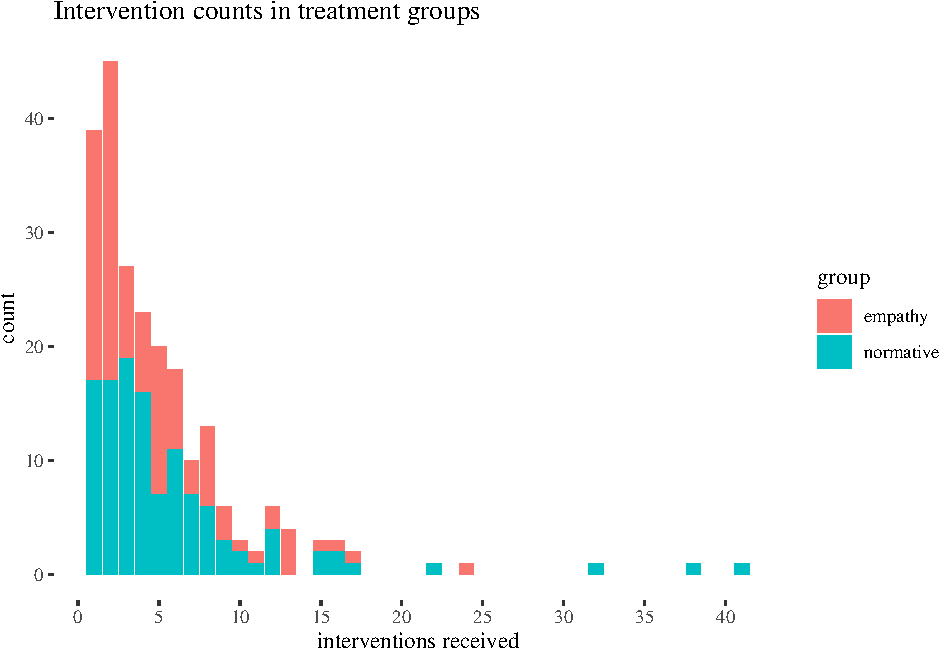
\includegraphics[width=1\linewidth]{bayesianReport3_files/figure-latex/treatmentHist-1} \end{center}
\normalsize

\todo{Note there were much more empathetic interventions, this needs an explanation}

\todo{Question: intervention counts by group}

Second, when we look at the distribution of standardized difference in
attacks, when restricted to (-1,1), the peaks of distributions are
shifted a bit, with lowest median for the normative group, but not too
much:

\vspace{1mm}
\footnotesize

\begin{Shaded}
\begin{Highlighting}[]
\NormalTok{violAdiffS }\OtherTok{\textless{}{-}} \FunctionTok{ggplot}\NormalTok{(summaries, }\FunctionTok{aes}\NormalTok{(}\AttributeTok{x=}\NormalTok{group, }\AttributeTok{y =}\NormalTok{ AdiffS))}\SpecialCharTok{+}
  \FunctionTok{geom\_violin}\NormalTok{() }\SpecialCharTok{+}\FunctionTok{theme\_tufte}\NormalTok{() }
\NormalTok{violJoint }\OtherTok{\textless{}{-}} \FunctionTok{ggarrange}\NormalTok{(violAdiffS}\SpecialCharTok{+}\FunctionTok{ggtitle}\NormalTok{(}\StringTok{"whole range"}\NormalTok{),}
\NormalTok{              violAdiffS }\SpecialCharTok{+} \FunctionTok{ylim}\NormalTok{(}\FunctionTok{c}\NormalTok{(}\SpecialCharTok{{-}}\DecValTok{1}\NormalTok{,}\DecValTok{1}\NormalTok{))}\SpecialCharTok{+}\FunctionTok{geom\_boxplot}\NormalTok{(}\AttributeTok{width =}\NormalTok{ .}\DecValTok{2}\NormalTok{)}\SpecialCharTok{+}
              \FunctionTok{ggtitle}\NormalTok{(}\StringTok{"restricted to ({-}1,1)"}\NormalTok{)) }
\end{Highlighting}
\end{Shaded}

\begin{verbatim}
## Warning: Removed 58 rows containing non-finite values (stat_ydensity).
\end{verbatim}

\begin{verbatim}
## Warning: Removed 58 rows containing non-finite values (stat_boxplot).
\end{verbatim}

\begin{Shaded}
\begin{Highlighting}[]
\NormalTok{violJointTitled }\OtherTok{\textless{}{-}} \FunctionTok{annotate\_figure}\NormalTok{(violJoint, }
  \AttributeTok{top =} \FunctionTok{text\_grob}\NormalTok{(}\StringTok{"Empirical distribution of change in attacks (standardized)"}\NormalTok{,}
                  \AttributeTok{size =} \DecValTok{12}\NormalTok{))}
\NormalTok{violJointTitled}
\end{Highlighting}
\end{Shaded}

\begin{center}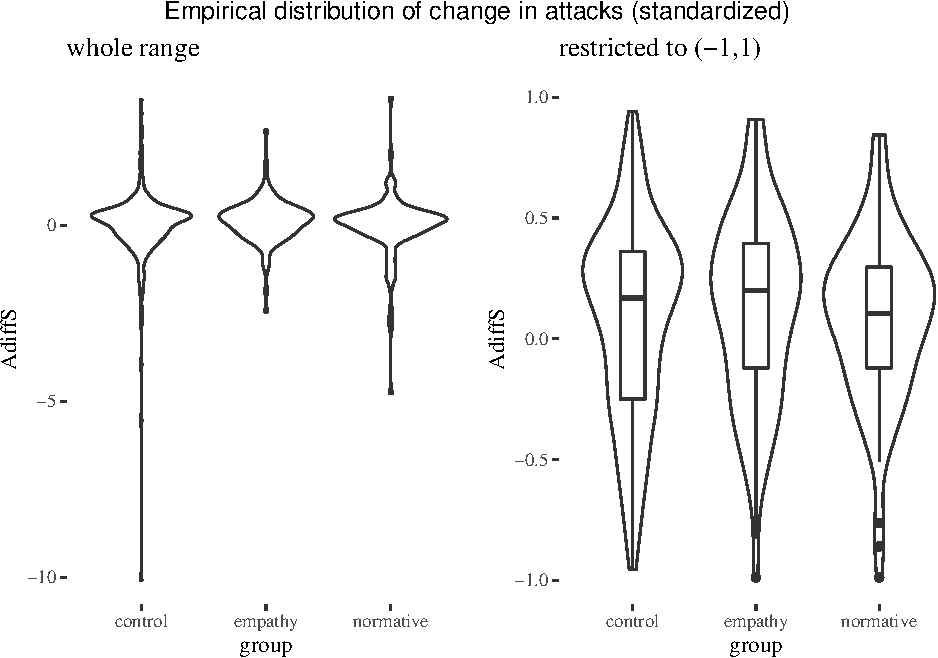
\includegraphics[width=1\linewidth]{bayesianReport3_files/figure-latex/violEmpiricalAdiff-1} \end{center}
\normalsize

Analogous plot for comments does not reveal this slight downward shift
for normative, but otherwise the visualisation migth suggest no strong
impact of interventions on attacks, and no impact on comments.

\vspace{1mm}
\footnotesize

\begin{Shaded}
\begin{Highlighting}[]
\NormalTok{violCdiffS }\OtherTok{\textless{}{-}} \FunctionTok{ggplot}\NormalTok{(summaries, }\FunctionTok{aes}\NormalTok{(}\AttributeTok{x=}\NormalTok{group, }\AttributeTok{y =}\NormalTok{ CdiffS))}\SpecialCharTok{+}
  \FunctionTok{geom\_violin}\NormalTok{() }\SpecialCharTok{+}\FunctionTok{theme\_tufte}\NormalTok{() }
\NormalTok{violJointC }\OtherTok{\textless{}{-}} \FunctionTok{ggarrange}\NormalTok{(violCdiffS}\SpecialCharTok{+}\FunctionTok{ggtitle}\NormalTok{(}\StringTok{"whole range"}\NormalTok{),}
\NormalTok{              violCdiffS }\SpecialCharTok{+} \FunctionTok{ylim}\NormalTok{(}\FunctionTok{c}\NormalTok{(}\SpecialCharTok{{-}}\DecValTok{1}\NormalTok{,}\DecValTok{1}\NormalTok{))}\SpecialCharTok{+}\FunctionTok{geom\_boxplot}\NormalTok{(}\AttributeTok{width =}\NormalTok{ .}\DecValTok{2}\NormalTok{)}\SpecialCharTok{+}
              \FunctionTok{ggtitle}\NormalTok{(}\StringTok{"restricted to ({-}1,1)"}\NormalTok{)) }
\end{Highlighting}
\end{Shaded}

\begin{verbatim}
## Warning: Removed 90 rows containing non-finite values (stat_ydensity).
\end{verbatim}

\begin{verbatim}
## Warning: Removed 90 rows containing non-finite values (stat_boxplot).
\end{verbatim}

\begin{Shaded}
\begin{Highlighting}[]
\NormalTok{violJointCTitled }\OtherTok{\textless{}{-}} \FunctionTok{annotate\_figure}\NormalTok{(violJoint, }
  \AttributeTok{top =} \FunctionTok{text\_grob}\NormalTok{(}\StringTok{"Empirical distribution of change in comments (standardized)"}\NormalTok{,}
                  \AttributeTok{size =} \DecValTok{12}\NormalTok{))}
\NormalTok{violJointCTitled}
\end{Highlighting}
\end{Shaded}

\begin{center}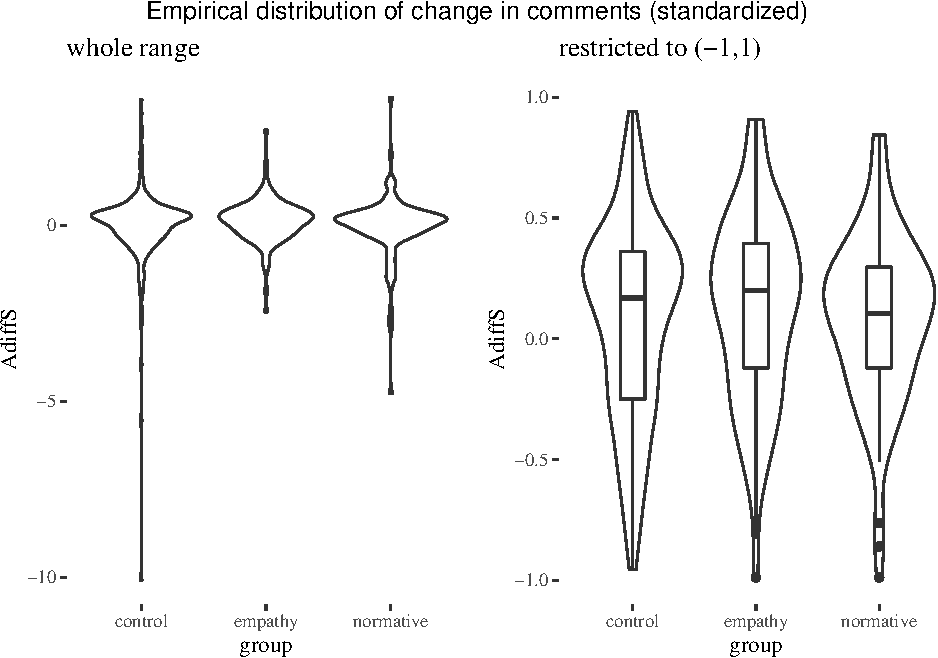
\includegraphics[width=1\linewidth]{bayesianReport3_files/figure-latex/violEpmiricalCdiff-1} \end{center}
\normalsize

However, plotting changes against intervention counts reveals that
restricting attention to various activity levels drastically changes the
regression lines.

\vspace{1mm}
\footnotesize

\begin{Shaded}
\begin{Highlighting}[]
\NormalTok{icplot1 }\OtherTok{\textless{}{-}} \FunctionTok{ggplot}\NormalTok{(summaries, }\FunctionTok{aes}\NormalTok{(}\AttributeTok{x =}\NormalTok{ IC, }\AttributeTok{y =}\NormalTok{ AdiffS, }\AttributeTok{color =}\NormalTok{ group, }\AttributeTok{fill =}\NormalTok{ group))}\SpecialCharTok{+}
  \FunctionTok{geom\_jitter}\NormalTok{(}\AttributeTok{alpha =} \FloatTok{0.6}\NormalTok{, }\AttributeTok{size =}\NormalTok{.}\DecValTok{8}\NormalTok{)}\SpecialCharTok{+}\FunctionTok{theme\_tufte}\NormalTok{()}\SpecialCharTok{+}
  \FunctionTok{geom\_smooth}\NormalTok{(}\AttributeTok{alpha =} \FloatTok{0.2}\NormalTok{, }\AttributeTok{method =} \StringTok{"lm"}\NormalTok{)}\SpecialCharTok{+}
  \FunctionTok{xlim}\NormalTok{(}\FunctionTok{c}\NormalTok{(}\DecValTok{0}\NormalTok{,}\DecValTok{25}\NormalTok{))}\SpecialCharTok{+}\FunctionTok{ylim}\NormalTok{(}\FunctionTok{c}\NormalTok{(}\SpecialCharTok{{-}}\DecValTok{2}\NormalTok{,}\DecValTok{2}\NormalTok{))}\SpecialCharTok{+}
  \FunctionTok{ggtitle}\NormalTok{(}\StringTok{"sd restricted to ({-}2,2)"}\NormalTok{)}\SpecialCharTok{+}
  \FunctionTok{theme}\NormalTok{(}\AttributeTok{legend.position =} \FunctionTok{c}\NormalTok{(}\FloatTok{0.65}\NormalTok{, }\FloatTok{0.1}\NormalTok{))}

\NormalTok{icplot2 }\OtherTok{\textless{}{-}}  \FunctionTok{ggplot}\NormalTok{(summaries, }\FunctionTok{aes}\NormalTok{(}\AttributeTok{x =}\NormalTok{ IC, }\AttributeTok{y =}\NormalTok{ AdiffS, }\AttributeTok{color =}\NormalTok{ group, }\AttributeTok{fill =}\NormalTok{ group))}\SpecialCharTok{+}
  \FunctionTok{geom\_jitter}\NormalTok{(}\AttributeTok{alpha =} \FloatTok{0.6}\NormalTok{, }\AttributeTok{size =}\NormalTok{.}\DecValTok{8}\NormalTok{)}\SpecialCharTok{+}\FunctionTok{theme\_tufte}\NormalTok{()}\SpecialCharTok{+}
  \FunctionTok{geom\_smooth}\NormalTok{(}\AttributeTok{alpha =} \FloatTok{0.2}\NormalTok{, }\AttributeTok{method =} \StringTok{"lm"}\NormalTok{)}\SpecialCharTok{+}
  \FunctionTok{xlim}\NormalTok{(}\FunctionTok{c}\NormalTok{(}\DecValTok{0}\NormalTok{,}\DecValTok{25}\NormalTok{))}\SpecialCharTok{+}\FunctionTok{ylim}\NormalTok{(}\FunctionTok{c}\NormalTok{(}\SpecialCharTok{{-}}\DecValTok{1}\NormalTok{,}\DecValTok{1}\NormalTok{))}\SpecialCharTok{+}\FunctionTok{ggtitle}\NormalTok{(}\StringTok{"sd restricted to ({-}1,1)"}\NormalTok{)}\SpecialCharTok{+}
  \FunctionTok{theme}\NormalTok{(}\AttributeTok{legend.position =} \FunctionTok{c}\NormalTok{(}\FloatTok{0.65}\NormalTok{, }\FloatTok{0.1}\NormalTok{))}

\NormalTok{icplotJoint }\OtherTok{\textless{}{-}} \FunctionTok{ggarrange}\NormalTok{(icplot1, icplot2) }
\NormalTok{icplotTitled }\OtherTok{\textless{}{-}} \FunctionTok{annotate\_figure}\NormalTok{(icplotJoint, }
  \AttributeTok{top =} \FunctionTok{text\_grob}\NormalTok{(}\StringTok{"Change in attacks (standardized) vs interventions received"}\NormalTok{,  }\AttributeTok{size =} \DecValTok{12}\NormalTok{))}
\NormalTok{icplotTitled}
\end{Highlighting}
\end{Shaded}

\begin{center}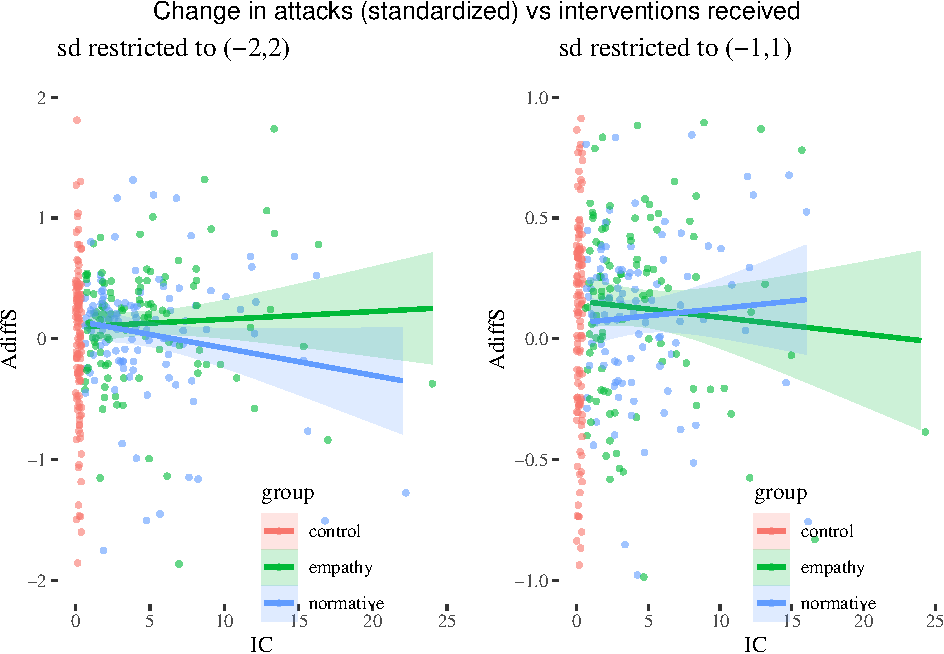
\includegraphics[width=1\linewidth]{bayesianReport3_files/figure-latex/ic-1} \end{center}
\normalsize

Some interactions are also suggested by the differences in linear
smoothing when attention is restricted when it comes to change in
comments.

\vspace{1mm}
\footnotesize

\begin{Shaded}
\begin{Highlighting}[]
\NormalTok{icCplot1 }\OtherTok{\textless{}{-}} \FunctionTok{ggplot}\NormalTok{(summaries, }\FunctionTok{aes}\NormalTok{(}\AttributeTok{x =}\NormalTok{ IC, }\AttributeTok{y =}\NormalTok{ CdiffS, }\AttributeTok{color =}\NormalTok{ group, }\AttributeTok{fill =}\NormalTok{ group))}\SpecialCharTok{+}
  \FunctionTok{geom\_jitter}\NormalTok{(}\AttributeTok{alpha =} \FloatTok{0.6}\NormalTok{, }\AttributeTok{size =}\NormalTok{.}\DecValTok{8}\NormalTok{)}\SpecialCharTok{+}\FunctionTok{theme\_tufte}\NormalTok{()}\SpecialCharTok{+}
  \FunctionTok{geom\_smooth}\NormalTok{(}\AttributeTok{alpha =} \FloatTok{0.2}\NormalTok{, }\AttributeTok{method =} \StringTok{"lm"}\NormalTok{)}\SpecialCharTok{+}
  \FunctionTok{xlim}\NormalTok{(}\FunctionTok{c}\NormalTok{(}\DecValTok{0}\NormalTok{,}\DecValTok{25}\NormalTok{))}\SpecialCharTok{+}\FunctionTok{ylim}\NormalTok{(}\FunctionTok{c}\NormalTok{(}\SpecialCharTok{{-}}\DecValTok{2}\NormalTok{,}\DecValTok{2}\NormalTok{))}\SpecialCharTok{+}
  \FunctionTok{ggtitle}\NormalTok{(}\StringTok{"sd restricted to ({-}2,2)"}\NormalTok{)}\SpecialCharTok{+}
  \FunctionTok{theme}\NormalTok{(}\AttributeTok{legend.position =} \FunctionTok{c}\NormalTok{(}\FloatTok{0.65}\NormalTok{, }\FloatTok{0.1}\NormalTok{))}

\NormalTok{icCplot2 }\OtherTok{\textless{}{-}}  \FunctionTok{ggplot}\NormalTok{(summaries, }\FunctionTok{aes}\NormalTok{(}\AttributeTok{x =}\NormalTok{ IC, }\AttributeTok{y =}\NormalTok{ CdiffS, }\AttributeTok{color =}\NormalTok{ group, }\AttributeTok{fill =}\NormalTok{ group))}\SpecialCharTok{+}
  \FunctionTok{geom\_jitter}\NormalTok{(}\AttributeTok{alpha =} \FloatTok{0.6}\NormalTok{, }\AttributeTok{size =}\NormalTok{.}\DecValTok{8}\NormalTok{)}\SpecialCharTok{+}\FunctionTok{theme\_tufte}\NormalTok{()}\SpecialCharTok{+}
  \FunctionTok{geom\_smooth}\NormalTok{(}\AttributeTok{alpha =} \FloatTok{0.2}\NormalTok{, }\AttributeTok{method =} \StringTok{"lm"}\NormalTok{)}\SpecialCharTok{+}
  \FunctionTok{xlim}\NormalTok{(}\FunctionTok{c}\NormalTok{(}\DecValTok{0}\NormalTok{,}\DecValTok{25}\NormalTok{))}\SpecialCharTok{+}\FunctionTok{ylim}\NormalTok{(}\FunctionTok{c}\NormalTok{(}\SpecialCharTok{{-}}\DecValTok{1}\NormalTok{,}\DecValTok{1}\NormalTok{))}\SpecialCharTok{+}\FunctionTok{ggtitle}\NormalTok{(}\StringTok{"sd restricted to ({-}1,1)"}\NormalTok{)}\SpecialCharTok{+}
  \FunctionTok{theme}\NormalTok{(}\AttributeTok{legend.position =} \FunctionTok{c}\NormalTok{(}\FloatTok{0.65}\NormalTok{, }\FloatTok{0.1}\NormalTok{))}

\NormalTok{icCplotJoint }\OtherTok{\textless{}{-}} \FunctionTok{ggarrange}\NormalTok{(icCplot1, icCplot2) }
\NormalTok{icCplotTitled }\OtherTok{\textless{}{-}} \FunctionTok{annotate\_figure}\NormalTok{(icCplotJoint, }
  \AttributeTok{top =} \FunctionTok{text\_grob}\NormalTok{(}\StringTok{"Change in comments (standardized) vs interventions received"}\NormalTok{,}
   \AttributeTok{size =} \DecValTok{12}\NormalTok{))}
\NormalTok{icCplotTitled}
\end{Highlighting}
\end{Shaded}

\begin{center}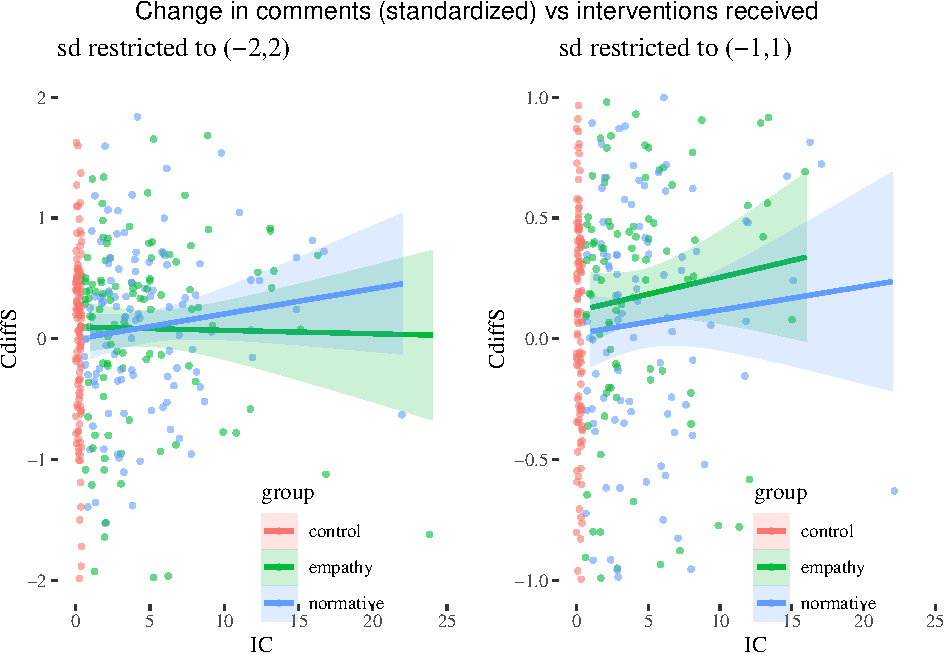
\includegraphics[width=1\linewidth]{bayesianReport3_files/figure-latex/icc-1} \end{center}
\normalsize

This suggests we should keep an eye out for interactions in the
analysis, and that the intial comparison of means or medians between
groups might be misleading if the effects in different volume groups are
different and cancel each other.

Now, let's inspect correlations between the variables involved in the
model:

\vspace{1mm}
\footnotesize

\begin{Shaded}
\begin{Highlighting}[]
\NormalTok{summariesCorr }\OtherTok{\textless{}{-}} \FunctionTok{select}\NormalTok{(summaries, IC, ABS, CBS, AAS, CAS, CDS, ADS)}
\FunctionTok{ggcorr}\NormalTok{(summariesCorr, }\AttributeTok{method =} \FunctionTok{c}\NormalTok{(}\StringTok{"pairwise"}\NormalTok{),}
       \AttributeTok{digits =} \DecValTok{4}\NormalTok{, }\AttributeTok{low =} \StringTok{"steelblue"}\NormalTok{, }\AttributeTok{mid =} \StringTok{"white"}\NormalTok{,}
       \AttributeTok{high =} \StringTok{"darkred"}\NormalTok{, }\AttributeTok{midpoint =}\DecValTok{0}\NormalTok{,}
       \AttributeTok{geom =} \StringTok{"tile"}\NormalTok{, }\AttributeTok{label =} \ConstantTok{TRUE}\NormalTok{, }\AttributeTok{label\_size=}\DecValTok{4}\NormalTok{, }\AttributeTok{label\_round =}\DecValTok{2}\NormalTok{, }\AttributeTok{layout.exp =}\DecValTok{1}\NormalTok{,}
       \AttributeTok{label\_alpha =} \ConstantTok{FALSE}\NormalTok{,}\AttributeTok{hjust =} \FloatTok{0.75}\NormalTok{)}
\end{Highlighting}
\end{Shaded}

\begin{center}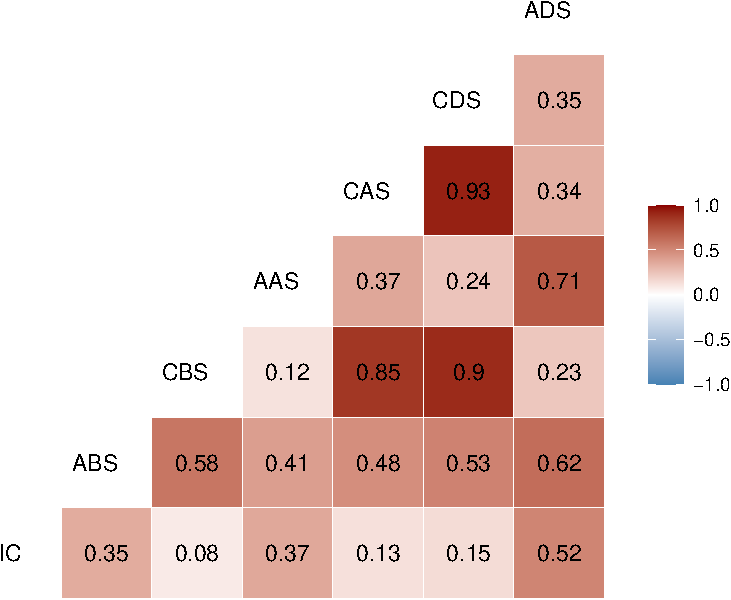
\includegraphics[width=1\linewidth]{bayesianReport3_files/figure-latex/correlations-1} \end{center}
\normalsize

This tells us that almost no predictors are strongly correlated, except
for pairs \textsf{CBS}-\textsf{CDS}, so we drop CDS from the analysis
and avoid using them in the same model to avoid multicolinearity issues.
These are just comments during the intervention period, which,
unsurprisingly are also a good proxy for comments before and comments
after.

\hypertarget{causal-inference}{%
\section{Causal inference}\label{causal-inference}}

To identify the right variables to condition (or not condition) on to
identify the causal effect of the interventions, we first need to think
about the causal structure of the problem. Here's a plausible causal
structure that we will be working with:

\vspace{1mm}
\footnotesize

\begin{Shaded}
\begin{Highlighting}[]
\NormalTok{dag }\OtherTok{\textless{}{-}} \FunctionTok{dagitty}\NormalTok{(}\StringTok{"}
\StringTok{  dag\{}
\StringTok{  CDS {-}\textgreater{} ADS {-}\textgreater{} IC  }
\StringTok{               U [unobserved]   }
\StringTok{               U {-}\textgreater{} CBS {-}\textgreater{} ABS  }
\StringTok{               U {-}\textgreater{} ABS        }
\StringTok{               U {-}\textgreater{} CDS {-}\textgreater{} ADS  }
\StringTok{               U {-}\textgreater{} ADS         }
\StringTok{               U {-}\textgreater{} CAS {-}\textgreater{} AAS    }
\StringTok{               U {-}\textgreater{} AAS                        }
\StringTok{               IC {-}\textgreater{} AAS        }
\StringTok{               IC {-}\textgreater{} CAS        }
\StringTok{               IT {-}\textgreater{} CAS        }
\StringTok{               IT {-}\textgreater{} AAS}
\StringTok{               CBS {-}\textgreater{} CDS {-}\textgreater{} CAS}
\StringTok{               ABS {-}\textgreater{} ADS {-}\textgreater{} AAS}
\StringTok{               \}"}\NormalTok{)}
\FunctionTok{coordinates}\NormalTok{(dag)}
\end{Highlighting}
\end{Shaded}

\begin{verbatim}
## $x
## AAS ABS ADS CAS CBS CDS  IC  IT   U 
##  NA  NA  NA  NA  NA  NA  NA  NA  NA 
## 
## $y
## AAS ABS ADS CAS CBS CDS  IC  IT   U 
##  NA  NA  NA  NA  NA  NA  NA  NA  NA
\end{verbatim}

\begin{Shaded}
\begin{Highlighting}[]
\FunctionTok{coordinates}\NormalTok{( dag ) }\OtherTok{\textless{}{-}} \FunctionTok{list}\NormalTok{( }\AttributeTok{x=}\FunctionTok{c}\NormalTok{(}\AttributeTok{CBS=}\DecValTok{0}\NormalTok{,}\AttributeTok{ABS=}\DecValTok{0}\NormalTok{,}\AttributeTok{CDS=}\DecValTok{1}\NormalTok{,}\AttributeTok{ADS=}\DecValTok{1}\NormalTok{, }\AttributeTok{CAS =} \DecValTok{2}\NormalTok{,}
                    \AttributeTok{AAS =} \DecValTok{2}\NormalTok{, }\AttributeTok{IT =} \FloatTok{1.5}\NormalTok{, }\AttributeTok{IC =} \FloatTok{1.5}\NormalTok{, }\AttributeTok{U =}\NormalTok{ .}\DecValTok{5}\NormalTok{) ,}
\AttributeTok{y=}\FunctionTok{c}\NormalTok{(}\AttributeTok{CBS =}\DecValTok{0}\NormalTok{,}\AttributeTok{ABS =} \DecValTok{1}\NormalTok{,}\AttributeTok{CDS =} \DecValTok{0}\NormalTok{,}\AttributeTok{ADS =} \DecValTok{1}\NormalTok{, }\AttributeTok{CAS =} \DecValTok{0}\NormalTok{, }\AttributeTok{AAS =} \DecValTok{1}\NormalTok{, }
    \AttributeTok{IT =}\NormalTok{ .}\DecValTok{3}\NormalTok{, }\AttributeTok{IC =}\NormalTok{ .}\DecValTok{7}\NormalTok{, }\AttributeTok{U =}\NormalTok{.}\DecValTok{5}\NormalTok{) )}
\FunctionTok{drawdag}\NormalTok{(dag)}
\end{Highlighting}
\end{Shaded}

\begin{center}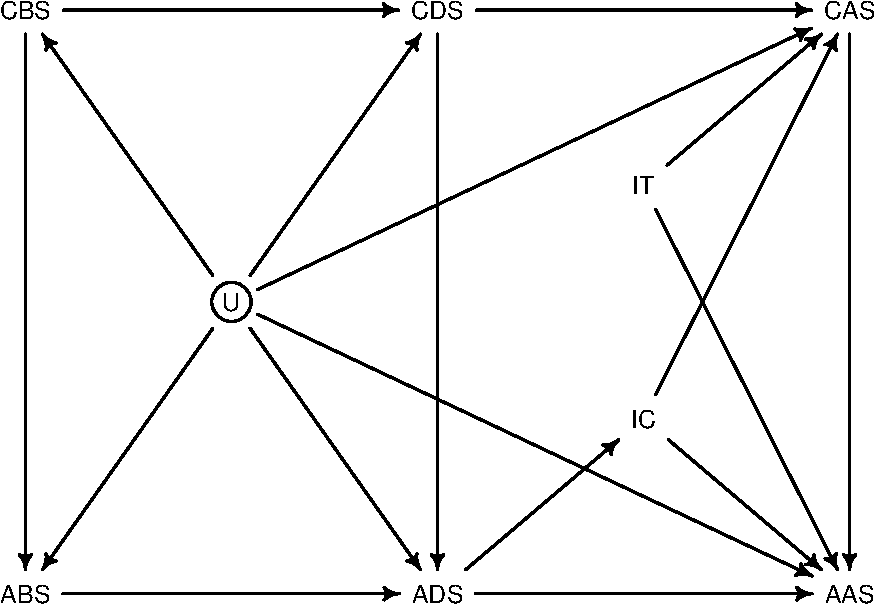
\includegraphics[width=0.8\linewidth]{bayesianReport3_files/figure-latex/dag1-1} \end{center}
\normalsize

Comments during impact attacks during, which trigger interventions.
Unmeasured user features cause comments before, which impact attacks
before, and also attacks before directly. Comments during (their impact
on ADS is areadly included) impact attacks during during directly and
comments after, which impact attacks after and attacks after directly.
Intervention count impacts attacks after and comments after. The same
directions of impact are included for intervention type. Finally,
comments through time are connected causally, and so are attacks.

We already know not to condition on CDS if we condition on CAS or CBS.
What else? \textsf{IT} has no bacwkard paths, but \textsf{IC} does.
Let's identify all paths from \textsf{IC} to \textsf{AAS}:

\vspace{1mm}
\footnotesize

\begin{Shaded}
\begin{Highlighting}[]
\FunctionTok{paths}\NormalTok{(dag, }\AttributeTok{from =} \FunctionTok{c}\NormalTok{(}\StringTok{"IC"}\NormalTok{), }\AttributeTok{to =} \StringTok{"AAS"}\NormalTok{)}
\end{Highlighting}
\end{Shaded}

\begin{verbatim}
## $paths
##  [1] "IC -> AAS"                                              
##  [2] "IC -> CAS -> AAS"                                       
##  [3] "IC -> CAS <- CDS -> ADS -> AAS"                         
##  [4] "IC -> CAS <- CDS -> ADS <- ABS <- CBS <- U -> AAS"      
##  [5] "IC -> CAS <- CDS -> ADS <- ABS <- U -> AAS"             
##  [6] "IC -> CAS <- CDS -> ADS <- U -> AAS"                    
##  [7] "IC -> CAS <- CDS <- CBS -> ABS -> ADS -> AAS"           
##  [8] "IC -> CAS <- CDS <- CBS -> ABS -> ADS <- U -> AAS"      
##  [9] "IC -> CAS <- CDS <- CBS -> ABS <- U -> AAS"             
## [10] "IC -> CAS <- CDS <- CBS -> ABS <- U -> ADS -> AAS"      
## [11] "IC -> CAS <- CDS <- CBS <- U -> AAS"                    
## [12] "IC -> CAS <- CDS <- CBS <- U -> ABS -> ADS -> AAS"      
## [13] "IC -> CAS <- CDS <- CBS <- U -> ADS -> AAS"             
## [14] "IC -> CAS <- CDS <- U -> AAS"                           
## [15] "IC -> CAS <- CDS <- U -> ABS -> ADS -> AAS"             
## [16] "IC -> CAS <- CDS <- U -> ADS -> AAS"                    
## [17] "IC -> CAS <- CDS <- U -> CBS -> ABS -> ADS -> AAS"      
## [18] "IC -> CAS <- IT -> AAS"                                 
## [19] "IC -> CAS <- U -> AAS"                                  
## [20] "IC -> CAS <- U -> ABS -> ADS -> AAS"                    
## [21] "IC -> CAS <- U -> ABS <- CBS -> CDS -> ADS -> AAS"      
## [22] "IC -> CAS <- U -> ADS -> AAS"                           
## [23] "IC -> CAS <- U -> CBS -> ABS -> ADS -> AAS"             
## [24] "IC -> CAS <- U -> CBS -> CDS -> ADS -> AAS"             
## [25] "IC -> CAS <- U -> CDS -> ADS -> AAS"                    
## [26] "IC -> CAS <- U -> CDS <- CBS -> ABS -> ADS -> AAS"      
## [27] "IC <- ADS -> AAS"                                       
## [28] "IC <- ADS <- ABS <- CBS -> CDS -> CAS -> AAS"           
## [29] "IC <- ADS <- ABS <- CBS -> CDS -> CAS <- IT -> AAS"     
## [30] "IC <- ADS <- ABS <- CBS -> CDS -> CAS <- U -> AAS"      
## [31] "IC <- ADS <- ABS <- CBS -> CDS <- U -> AAS"             
## [32] "IC <- ADS <- ABS <- CBS -> CDS <- U -> CAS -> AAS"      
## [33] "IC <- ADS <- ABS <- CBS -> CDS <- U -> CAS <- IT -> AAS"
## [34] "IC <- ADS <- ABS <- CBS <- U -> AAS"                    
## [35] "IC <- ADS <- ABS <- CBS <- U -> CAS -> AAS"             
## [36] "IC <- ADS <- ABS <- CBS <- U -> CAS <- IT -> AAS"       
## [37] "IC <- ADS <- ABS <- CBS <- U -> CDS -> CAS -> AAS"      
## [38] "IC <- ADS <- ABS <- CBS <- U -> CDS -> CAS <- IT -> AAS"
## [39] "IC <- ADS <- ABS <- U -> AAS"                           
## [40] "IC <- ADS <- ABS <- U -> CAS -> AAS"                    
## [41] "IC <- ADS <- ABS <- U -> CAS <- IT -> AAS"              
## [42] "IC <- ADS <- ABS <- U -> CBS -> CDS -> CAS -> AAS"      
## [43] "IC <- ADS <- ABS <- U -> CBS -> CDS -> CAS <- IT -> AAS"
## [44] "IC <- ADS <- ABS <- U -> CDS -> CAS -> AAS"             
## [45] "IC <- ADS <- ABS <- U -> CDS -> CAS <- IT -> AAS"       
## [46] "IC <- ADS <- CDS -> CAS -> AAS"                         
## [47] "IC <- ADS <- CDS -> CAS <- IT -> AAS"                   
## [48] "IC <- ADS <- CDS -> CAS <- U -> AAS"                    
## [49] "IC <- ADS <- CDS <- CBS -> ABS <- U -> AAS"             
## [50] "IC <- ADS <- CDS <- CBS -> ABS <- U -> CAS -> AAS"      
## [51] "IC <- ADS <- CDS <- CBS -> ABS <- U -> CAS <- IT -> AAS"
## [52] "IC <- ADS <- CDS <- CBS <- U -> AAS"                    
## [53] "IC <- ADS <- CDS <- CBS <- U -> CAS -> AAS"             
## [54] "IC <- ADS <- CDS <- CBS <- U -> CAS <- IT -> AAS"       
## [55] "IC <- ADS <- CDS <- U -> AAS"                           
## [56] "IC <- ADS <- CDS <- U -> CAS -> AAS"                    
## [57] "IC <- ADS <- CDS <- U -> CAS <- IT -> AAS"              
## [58] "IC <- ADS <- U -> AAS"                                  
## [59] "IC <- ADS <- U -> ABS <- CBS -> CDS -> CAS -> AAS"      
## [60] "IC <- ADS <- U -> ABS <- CBS -> CDS -> CAS <- IT -> AAS"
## [61] "IC <- ADS <- U -> CAS -> AAS"                           
## [62] "IC <- ADS <- U -> CAS <- IT -> AAS"                     
## [63] "IC <- ADS <- U -> CBS -> CDS -> CAS -> AAS"             
## [64] "IC <- ADS <- U -> CBS -> CDS -> CAS <- IT -> AAS"       
## [65] "IC <- ADS <- U -> CDS -> CAS -> AAS"                    
## [66] "IC <- ADS <- U -> CDS -> CAS <- IT -> AAS"              
## 
## $open
##  [1]  TRUE  TRUE FALSE FALSE FALSE FALSE FALSE FALSE FALSE FALSE FALSE FALSE
## [13] FALSE FALSE FALSE FALSE FALSE FALSE FALSE FALSE FALSE FALSE FALSE FALSE
## [25] FALSE FALSE  TRUE  TRUE FALSE FALSE FALSE FALSE FALSE  TRUE  TRUE FALSE
## [37]  TRUE FALSE  TRUE  TRUE FALSE  TRUE FALSE  TRUE FALSE  TRUE FALSE FALSE
## [49] FALSE FALSE FALSE  TRUE  TRUE FALSE  TRUE  TRUE FALSE  TRUE FALSE FALSE
## [61]  TRUE FALSE  TRUE FALSE  TRUE FALSE
\end{verbatim}

\normalsize

Crucially, all backdoor paths go through \textsf{ADS}, which then
becomes either a fork or a pipe, so all backdoor paths can be closed by
conditioning on \textsf{ADS}. Moreover there is only one directed
indirect path, it goes through \textsf{CAS}, so we should not condition
on it if we are to identify causal effect on attacks mediated by impact
on comments (unless we care about the direct effect of \textsf{IC} and
\textsf{IT} on \textsf{AAS}, but that's a separate question). This is in
line with the adjustment set identified algorithmically.

\vspace{1mm}
\footnotesize

\begin{Shaded}
\begin{Highlighting}[]
\FunctionTok{adjustmentSets}\NormalTok{(dag, }\AttributeTok{exposure =} \FunctionTok{c}\NormalTok{(}\StringTok{"IC"}\NormalTok{, }\StringTok{"IT"}\NormalTok{), }\AttributeTok{outcome =} \StringTok{"AAS"}\NormalTok{, }\AttributeTok{type =} \StringTok{"all"}\NormalTok{)}
\end{Highlighting}
\end{Shaded}

\begin{verbatim}
## { ADS }
## { ABS, ADS }
## { ADS, CBS }
## { ABS, ADS, CBS }
## { ADS, CDS }
## { ABS, ADS, CDS }
## { ADS, CBS, CDS }
## { ABS, ADS, CBS, CDS }
## { ADS, U }
## { ABS, ADS, U }
## { ADS, CBS, U }
## { ABS, ADS, CBS, U }
## { ADS, CDS, U }
## { ABS, ADS, CDS, U }
## { ADS, CBS, CDS, U }
## { ABS, ADS, CBS, CDS, U }
\end{verbatim}

\normalsize

The situation is different when it comes to evaluating the \emph{direct}
effect of intervention. Then, we also need to block indirect causal
paths from the intervention to the outcome. For such an evaluation we
need to also condition on \textsf{CAS}, which is what we will do when we
turn to the study of the direct effects of the interventions.

In fact, we will be predicting the difference between attacks before and
after, and the difference between comments, before and after. Let's add
them to the dag to double-check our selection of variables.

\begin{Shaded}
\begin{Highlighting}[]
\NormalTok{dag2 }\OtherTok{\textless{}{-}} \FunctionTok{dagitty}\NormalTok{(}\StringTok{"}
\StringTok{  dag\{}
\StringTok{                CDS {-}\textgreater{} ADS {-}\textgreater{} IC  }
\StringTok{                U [unobserved]   }
\StringTok{                U {-}\textgreater{} CBS {-}\textgreater{} ABS  }
\StringTok{                U {-}\textgreater{} ABS        }
\StringTok{                U {-}\textgreater{} CDS {-}\textgreater{} ADS  }
\StringTok{                U {-}\textgreater{} ADS         }
\StringTok{                U {-}\textgreater{} CAS {-}\textgreater{} AAS    }
\StringTok{                U {-}\textgreater{} AAS                        }
\StringTok{                IC {-}\textgreater{} AAS        }
\StringTok{                IC {-}\textgreater{} CAS        }
\StringTok{                IT {-}\textgreater{} CAS        }
\StringTok{                IT {-}\textgreater{} AAS}
\StringTok{                CBS {-}\textgreater{} CDS {-}\textgreater{} CAS}
\StringTok{                ABS {-}\textgreater{} ADS {-}\textgreater{} AAS}
\StringTok{                ABS {-}\textgreater{} AdiffS}
\StringTok{                AAS {-}\textgreater{} AdiffS}
\StringTok{                CBS {-}\textgreater{} CdiffS}
\StringTok{                CAS {-}\textgreater{} CdiffS}
\StringTok{                \}"}\NormalTok{)}
\FunctionTok{coordinates}\NormalTok{( dag2 ) }\OtherTok{\textless{}{-}} \FunctionTok{list}\NormalTok{( }\AttributeTok{x=}\FunctionTok{c}\NormalTok{(}\AttributeTok{CBS=}\DecValTok{0}\NormalTok{,}\AttributeTok{ABS=}\DecValTok{0}\NormalTok{,}\AttributeTok{CDS=}\DecValTok{1}\NormalTok{,}\AttributeTok{ADS=}\DecValTok{1}\NormalTok{,}
    \AttributeTok{CAS =} \DecValTok{2}\NormalTok{, }\AttributeTok{AAS =} \DecValTok{2}\NormalTok{, }\AttributeTok{IT =} \FloatTok{1.5}\NormalTok{, }\AttributeTok{IC =} \FloatTok{1.5}\NormalTok{, }\AttributeTok{U =}\NormalTok{ .}\DecValTok{5}\NormalTok{, }\AttributeTok{AdiffS=} \FloatTok{2.5}\NormalTok{, }\AttributeTok{CdiffS =} \FloatTok{2.5}\NormalTok{) ,}
\AttributeTok{y=}\FunctionTok{c}\NormalTok{(}\AttributeTok{CBS =}\DecValTok{0}\NormalTok{,}\AttributeTok{ABS =} \DecValTok{1}\NormalTok{,}\AttributeTok{CDS =} \DecValTok{0}\NormalTok{,}\AttributeTok{ADS =} \DecValTok{1}\NormalTok{, }\AttributeTok{CAS =} \DecValTok{0}\NormalTok{, }\AttributeTok{AAS =} \DecValTok{1}\NormalTok{, }\AttributeTok{IT =}\NormalTok{ .}\DecValTok{3}\NormalTok{, }\AttributeTok{IC =}\NormalTok{ .}\DecValTok{7}\NormalTok{, }\AttributeTok{U =}\NormalTok{.}\DecValTok{5}\NormalTok{, }\AttributeTok{CdiffS =} \SpecialCharTok{{-}}\NormalTok{.}\DecValTok{2}\NormalTok{,  }\AttributeTok{AdiffS =} \FloatTok{1.2}\NormalTok{) )}

\FunctionTok{drawdag}\NormalTok{(dag2)}
\FunctionTok{adjustmentSets}\NormalTok{(dag2, }\AttributeTok{exposure =} \FunctionTok{c}\NormalTok{(}\StringTok{"IC"}\NormalTok{, }\StringTok{"IT"}\NormalTok{), }\AttributeTok{outcome =} \StringTok{"AdiffS"}\NormalTok{, }\AttributeTok{type =} \StringTok{"canonical"}\NormalTok{)}
\end{Highlighting}
\end{Shaded}

\begin{verbatim}
## { ABS, ADS, CBS, CDS }
\end{verbatim}

\begin{center}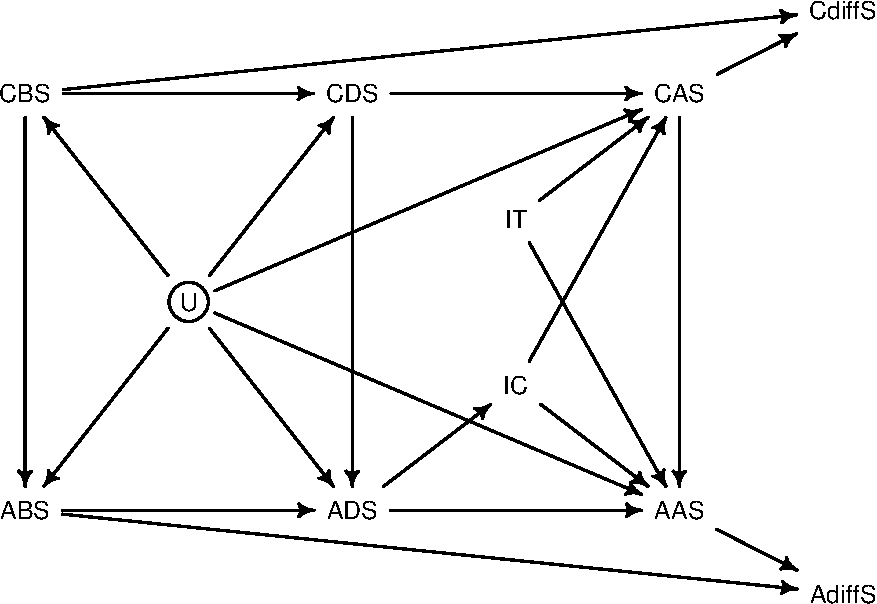
\includegraphics[width=0.8\linewidth]{bayesianReport3_files/figure-latex/dag2-1} \end{center}

Finding a maximal sensible set (canonical) of covariates suggests
inlcuding \textsf{CDS} and \textsf{ABS}. As already discussed, we do not
include \textsf{CDS} because of its strong correlation with
\textsf{CBS}. We also do not condition on \textsf{ABS}---not only
because it has a pretty strong correlation with another predictor
(\textsf{ADS}), but rather mainly because it is used to define the
output variable. In such a set-up, of course that a model including
\textsf{ABS} would have better predictive power, but since a
definitional connection is present, thinking that its inclusion in the
model tells us something about causality would be misled.

It's open season for the other variables (and interactions between
them), and our decision to include them in the model will be guided by
information-theoretic criteria of predictive power.

We will focus on a class of additive models where the outcome variable
is normally distributed around the predicted mean, which is a linear
function of predictors (possibly with some interactions). To spoil the
story, we will end up using a model, whose specification is as follows:

\begin{align*}
\mathsf{AdiffS} & \sim \textsf{Norm}(\mu, \sigma)\\
\mu_i & = \alpha + \beta_{\mathsf{ADS}}[\mathsf{group}_i]\times \mathsf{ADS} + \beta_{\mathsf{group}_i}  +
 \beta_{\mathsf{IC}}[\mathsf{group}_i]\times \mathsf{IC} + \\
 & + \beta_{\mathsf{ADSIC}}\times \mathsf{ADS} \times \mathsf{IC} + \beta_{\mathsf{CBS}}[\mathsf{group}_i] \times \mathsf{CBS}\\
 \alpha & \sim \textsf{Norm}(0,.3)\\
\beta_{\mathsf{ADS}}[\mathsf{group}_i] & \sim \textsf{Norm}(0,.3)\\
\beta_{\mathsf{group}_i} & \sim \textsf{Norm}(0,.3)\\
\beta_{\mathsf{IC}}[\mathsf{group}_i] & \sim \textsf{Norm}(0,.3)\\
 \beta_{\mathsf{ADSIC}} & \sim \textsf{Norm}(0,.3)\\
 \beta_{\mathsf{CBS}}[\mathsf{group}_i]& \sim \textsf{Norm}(0,.3)\\
\end{align*}

That is, we take the resulting mean to be the result of the general
average (\(\alpha\)) and the impact of the following coefficients:
group-specific coefficient for \textsf{ADS}, group coefficient,
group-specific coefficient for \textsf{IC}, interaction coefficient for
\textsf{ADS} and \textsf{IC}, and group-specific coeffient for
\textsf{CBS}. This is plausible prima facie which group a user belongs
to might have impact on how attacks during the treatment is related to
attacks after, the role of the intervention count, and the role of
comments before. Moreover, the levels of agressive behavior displayed by
the user during treament might have impact on the role played by the
intervention count. Later on we will see that there are
information-theoretic reasons to include these interactions.

Now for the priors. One might be suspicious of \(\sigma =.3\) we
employed and suggest using standard normal distributions with
\(\sigma = 1\) instead. However, a quick prior predictive check shows
that this results in insanely wide priors that are competely
unrealistic. (For computational reasons, instead of running the
simulations, we load pre-compiled models, but we include the code used
to build them).

\vspace{1mm}
\footnotesize

\begin{Shaded}
\begin{Highlighting}[]
\CommentTok{\# building model with sd=1}
\CommentTok{\# InteractionsModelDiffSD1 \textless{}{-} ulam(}
\CommentTok{\#   alist(}
\CommentTok{\#     AdiffS \textasciitilde{} dnorm( mu, sigma ),}
\CommentTok{\#     mu \textless{}{-} a + bADS[groupID] * ADS +  bIT[groupID] + bIC[groupID] * IC+}
\CommentTok{\#     bADSIC * ADS * IC+ bCBS[groupID] *CBS,}
\CommentTok{\#     a \textasciitilde{} dnorm (0,1),}
\CommentTok{\#     bADS[groupID] \textasciitilde{} dnorm(0,1),}
\CommentTok{\#     bADSIC \textasciitilde{} dnorm(0,1),}
\CommentTok{\#     bCBS[groupID] \textasciitilde{} dnorm(0,1),}
\CommentTok{\#     bIT[groupID] \textasciitilde{} dnorm(0,1),}
\CommentTok{\#     bIC[groupID] \textasciitilde{} dnorm(0,1),}
\CommentTok{\#     sigma  \textasciitilde{} dexp(1)}
\CommentTok{\#   ), }
\CommentTok{\#   data = summaries}
\CommentTok{\# )}
\CommentTok{\# }
\CommentTok{\# saveRDS(InteractionsModelDiffSD1, file = "models/InteractionsModelDiffSD1.rds")}
\NormalTok{InteractionsModelDiffSD1 }\OtherTok{\textless{}{-}} \FunctionTok{readRDS}\NormalTok{(}\AttributeTok{file =} \StringTok{"models/InteractionsModelDiffSD1.rds"}\NormalTok{)}


\CommentTok{\#now model with prior sd = .3}
\CommentTok{\# InteractionsModelDiff \textless{}{-} ulam(}
\CommentTok{\#   alist(}
\CommentTok{\#     AdiffS \textasciitilde{} dnorm( mu, sigma ),}
\CommentTok{\#     mu \textless{}{-} a + bADS[groupID] * ADS +  bIT[groupID] + bIC[groupID] * IC +}
\CommentTok{\#     bADSIC * ADS * IC+ bCBS[groupID] *CBS,}
\CommentTok{\#     a \textasciitilde{} dnorm (0,0.3),}
\CommentTok{\#     bADS[groupID] \textasciitilde{} dnorm(0,.3),}
\CommentTok{\#     bADSIC \textasciitilde{} dnorm(0,.3),}
\CommentTok{\#     bCBS[groupID] \textasciitilde{} dnorm(0,.3),}
\CommentTok{\#     bIT[groupID] \textasciitilde{} dnorm(0,.3),}
\CommentTok{\#     bIC[groupID] \textasciitilde{} dnorm(0,.3),}
\CommentTok{\#     sigma  \textasciitilde{} dexp(1)}
\CommentTok{\#   ), }
\CommentTok{\#   data = summaries}
\CommentTok{\# )}

\CommentTok{\#saveRDS(InteractionsModelDiff, file = "models/InteractionsModelDiff.rds")}

\NormalTok{InteractionsModelDiff }\OtherTok{\textless{}{-}} \FunctionTok{readRDS}\NormalTok{(}\AttributeTok{file =} \StringTok{"models/InteractionsModelDiff.rds"}\NormalTok{)}

\DocumentationTok{\#\#prior predictive checks sd =1}
\NormalTok{ADS }\OtherTok{\textless{}{-}} \DecValTok{0}
\NormalTok{CBS }\OtherTok{\textless{}{-}} \DecValTok{0}
\NormalTok{groupID }\OtherTok{\textless{}{-}} \DecValTok{1}\SpecialCharTok{:}\DecValTok{3}
\NormalTok{IC }\OtherTok{\textless{}{-}} \DecValTok{5}  \CommentTok{\#mean for interventions in treatment}
\NormalTok{data }\OtherTok{\textless{}{-}} \FunctionTok{expand.grid}\NormalTok{(}\AttributeTok{ADS =}\NormalTok{ ADS,}\AttributeTok{groupID =}\NormalTok{ groupID, }\AttributeTok{CBS =}\NormalTok{ CBS, }\AttributeTok{IC =}\NormalTok{  IC)}
\NormalTok{prior }\OtherTok{\textless{}{-}} \FunctionTok{extract.prior}\NormalTok{(InteractionsModelDiffSD1, }\AttributeTok{n =} \FloatTok{1e4}\NormalTok{)}
\NormalTok{mu }\OtherTok{\textless{}{-}} \FunctionTok{link}\NormalTok{( InteractionsModelDiffSD1 , }\AttributeTok{post=}\NormalTok{prior , }\AttributeTok{data=}\NormalTok{data ) }
\FunctionTok{colnames}\NormalTok{(mu) }\OtherTok{\textless{}{-}} \FunctionTok{levels}\NormalTok{(summaries}\SpecialCharTok{$}\NormalTok{group)}
\NormalTok{muLong }\OtherTok{\textless{}{-}} \FunctionTok{melt}\NormalTok{(mu)}
\FunctionTok{colnames}\NormalTok{(muLong) }\OtherTok{\textless{}{-}} \FunctionTok{c}\NormalTok{(}\StringTok{"id"}\NormalTok{, }\StringTok{"group"}\NormalTok{, }\StringTok{"AdiffS"}\NormalTok{)}

\NormalTok{priorGroupsSD1 }\OtherTok{\textless{}{-}} \FunctionTok{ggplot}\NormalTok{(muLong)}\SpecialCharTok{+}
  \FunctionTok{geom\_violin}\NormalTok{(}\FunctionTok{aes}\NormalTok{(}\AttributeTok{x =}\NormalTok{ group, }\AttributeTok{y =}\NormalTok{ AdiffS))}\SpecialCharTok{+}
  \FunctionTok{theme\_tufte}\NormalTok{()}\SpecialCharTok{+}\FunctionTok{xlab}\NormalTok{(}\StringTok{""}\NormalTok{)}\SpecialCharTok{+}
  \FunctionTok{labs}\NormalTok{(}\AttributeTok{title =} \StringTok{"Simulated priors by group"}\NormalTok{,}
  \AttributeTok{subtitle =} \StringTok{"(at ADS = CBS = 0, IC at mean = 5, sd = 1)"}\NormalTok{)}\SpecialCharTok{+}
  \FunctionTok{ylab}\NormalTok{(}\StringTok{"change in attacks (standardized)"}\NormalTok{)}

\NormalTok{ADS }\OtherTok{\textless{}{-}} \DecValTok{0}
\NormalTok{CBS }\OtherTok{\textless{}{-}} \DecValTok{0}
\NormalTok{groupID }\OtherTok{\textless{}{-}} \DecValTok{1}\SpecialCharTok{:}\DecValTok{3}
\NormalTok{IC }\OtherTok{\textless{}{-}} \DecValTok{0}\SpecialCharTok{:}\DecValTok{20}
\NormalTok{data }\OtherTok{\textless{}{-}} \FunctionTok{expand.grid}\NormalTok{(}\AttributeTok{ADS =}\NormalTok{ ADS,}\AttributeTok{groupID =}\NormalTok{ groupID, }\AttributeTok{CBS =}\NormalTok{ CBS, }\AttributeTok{IC =}\NormalTok{  IC)}

\NormalTok{prior }\OtherTok{\textless{}{-}} \FunctionTok{extract.prior}\NormalTok{(InteractionsModelDiffSD1, }\AttributeTok{n =} \FloatTok{1e4}\NormalTok{)}
\end{Highlighting}
\end{Shaded}

\begin{verbatim}
## recompiling to avoid crashing R session
\end{verbatim}

\begin{Shaded}
\begin{Highlighting}[]
\NormalTok{mu }\OtherTok{\textless{}{-}} \FunctionTok{link}\NormalTok{(InteractionsModelDiffSD1 , }\AttributeTok{post=}\NormalTok{prior , }\AttributeTok{data=}\NormalTok{data ) }
\NormalTok{mu.mean }\OtherTok{\textless{}{-}} \FunctionTok{apply}\NormalTok{( mu , }\DecValTok{2}\NormalTok{, mean )}
\NormalTok{mu.HPDI }\OtherTok{\textless{}{-}} \FunctionTok{data.frame}\NormalTok{(}\FunctionTok{t}\NormalTok{(}\FunctionTok{apply}\NormalTok{( mu , }\DecValTok{2}\NormalTok{ , HPDI )))}
\NormalTok{priorDF }\OtherTok{\textless{}{-}} \FunctionTok{cbind}\NormalTok{(data, mu.mean, mu.HPDI)}
\NormalTok{priorDF}\SpecialCharTok{$}\NormalTok{groupID }\OtherTok{\textless{}{-}} \FunctionTok{as.factor}\NormalTok{(groupID)}
\FunctionTok{levels}\NormalTok{(priorDF}\SpecialCharTok{$}\NormalTok{groupID) }\OtherTok{\textless{}{-}} \FunctionTok{c}\NormalTok{(}\StringTok{"control"}\NormalTok{, }\StringTok{"empathy"}\NormalTok{, }\StringTok{"normative"}\NormalTok{)}
\FunctionTok{colnames}\NormalTok{(priorDF)[}\DecValTok{2}\NormalTok{]}\OtherTok{\textless{}{-}} \StringTok{"group"}


\NormalTok{priorICSD1  }\OtherTok{\textless{}{-}} \FunctionTok{ggplot}\NormalTok{(priorDF, }\FunctionTok{aes}\NormalTok{(}\AttributeTok{x =}\NormalTok{ IC, }\AttributeTok{y  =}\NormalTok{ mu.mean,  }\AttributeTok{fill =}\NormalTok{ group))}\SpecialCharTok{+}
  \FunctionTok{geom\_line}\NormalTok{()}\SpecialCharTok{+}\FunctionTok{geom\_ribbon}\NormalTok{(}\FunctionTok{aes}\NormalTok{(}\AttributeTok{ymin =}\NormalTok{ X.}\FloatTok{0.89}\NormalTok{, }\AttributeTok{ymax =}\NormalTok{ X0.}\FloatTok{89.}\NormalTok{), }\AttributeTok{alpha =} \FloatTok{0.2}\NormalTok{)}\SpecialCharTok{+}
  \FunctionTok{theme\_tufte}\NormalTok{()}\SpecialCharTok{+}\FunctionTok{ylab}\NormalTok{(}\StringTok{"change in attacks (standardized)"}\NormalTok{)}\SpecialCharTok{+}
  \FunctionTok{labs}\NormalTok{(}\AttributeTok{title =} \StringTok{"Simulated priors for AAS vs IC"}\NormalTok{,}
      \AttributeTok{subtitle =} \StringTok{"(at ADS = CBS = 0, sd = 1)"}\NormalTok{)}\SpecialCharTok{+}\FunctionTok{xlab}\NormalTok{(}\StringTok{"interventions"}\NormalTok{)}


\NormalTok{priorJoint1 }\OtherTok{\textless{}{-}} \FunctionTok{ggarrange}\NormalTok{(priorGroupsSD1,priorICSD1, }\AttributeTok{ncol =} \DecValTok{2}\NormalTok{) }
\NormalTok{priorJoint1Titled }\OtherTok{\textless{}{-}} \FunctionTok{annotate\_figure}\NormalTok{(priorJoint1, }
  \AttributeTok{top =} \FunctionTok{text\_grob}\NormalTok{(}\StringTok{"Predictive priors with sd=1 are insanely wide"}\NormalTok{,}
                  \AttributeTok{size =} \DecValTok{14}\NormalTok{))}
\NormalTok{priorJoint1Titled}
\end{Highlighting}
\end{Shaded}

\begin{center}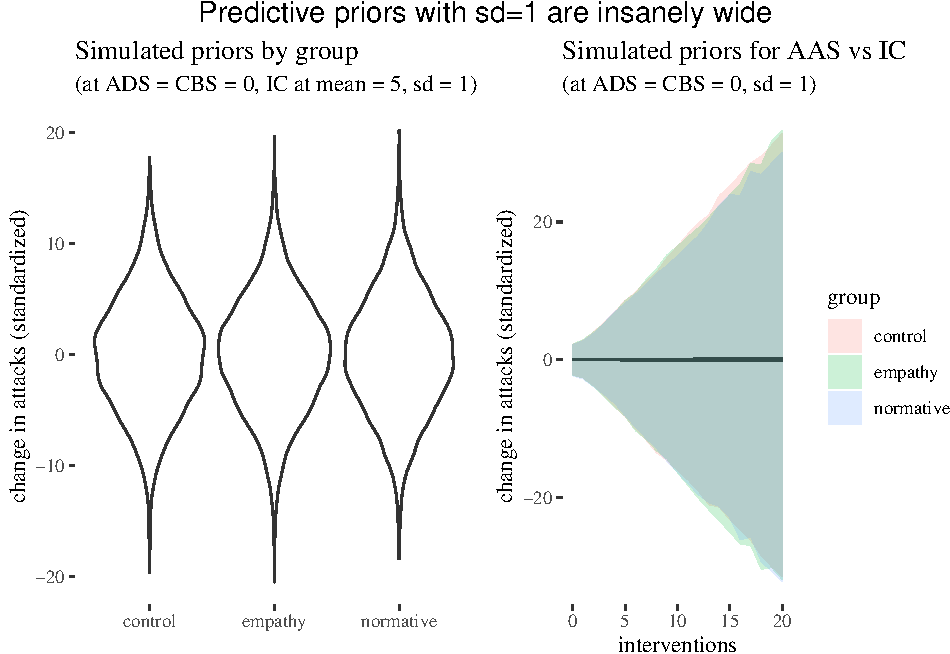
\includegraphics[width=1\linewidth]{bayesianReport3_files/figure-latex/priors1-1} \end{center}
\normalsize

Some experimentation leads to the value of \(\sigma =.3\), which leads
to the following priors:

\vspace{1mm}
\footnotesize

\begin{Shaded}
\begin{Highlighting}[]
\CommentTok{\#prior predictive check sd =.3}
\NormalTok{ADS }\OtherTok{\textless{}{-}} \DecValTok{0}
\NormalTok{CBS }\OtherTok{\textless{}{-}} \DecValTok{0}
\NormalTok{groupID }\OtherTok{\textless{}{-}} \DecValTok{1}\SpecialCharTok{:}\DecValTok{3}
\NormalTok{IC }\OtherTok{\textless{}{-}} \DecValTok{5}  \CommentTok{\#mean for interventions in treatment}
\NormalTok{data }\OtherTok{\textless{}{-}} \FunctionTok{expand.grid}\NormalTok{(}\AttributeTok{ADS =}\NormalTok{ ADS,}\AttributeTok{groupID =}\NormalTok{ groupID, }\AttributeTok{CBS =}\NormalTok{ CBS, }\AttributeTok{IC =}\NormalTok{  IC)}
\NormalTok{prior }\OtherTok{\textless{}{-}} \FunctionTok{extract.prior}\NormalTok{(InteractionsModelDiff, }\AttributeTok{n =} \FloatTok{1e4}\NormalTok{)}
\NormalTok{mu }\OtherTok{\textless{}{-}} \FunctionTok{link}\NormalTok{(InteractionsModelDiff , }\AttributeTok{post=}\NormalTok{prior , }\AttributeTok{data=}\NormalTok{data ) }
\FunctionTok{colnames}\NormalTok{(mu) }\OtherTok{\textless{}{-}} \FunctionTok{levels}\NormalTok{(summaries}\SpecialCharTok{$}\NormalTok{group)}
\NormalTok{muLong }\OtherTok{\textless{}{-}} \FunctionTok{melt}\NormalTok{(mu)}
\FunctionTok{colnames}\NormalTok{(muLong) }\OtherTok{\textless{}{-}} \FunctionTok{c}\NormalTok{(}\StringTok{"id"}\NormalTok{, }\StringTok{"group"}\NormalTok{, }\StringTok{"AdiffS"}\NormalTok{)}
\FunctionTok{head}\NormalTok{(muLong)}

\NormalTok{priorGroupSD03 }\OtherTok{\textless{}{-}} \FunctionTok{ggplot}\NormalTok{(muLong)}\SpecialCharTok{+}
  \FunctionTok{geom\_violin}\NormalTok{(}\FunctionTok{aes}\NormalTok{(}\AttributeTok{x =}\NormalTok{ group, }\AttributeTok{y =}\NormalTok{ AdiffS))}\SpecialCharTok{+}\FunctionTok{theme\_tufte}\NormalTok{()}\SpecialCharTok{+}
  \FunctionTok{xlab}\NormalTok{(}\StringTok{""}\NormalTok{)}\SpecialCharTok{+}
  \FunctionTok{labs}\NormalTok{(}\AttributeTok{title =} \StringTok{"Simulated priors  by group"}\NormalTok{, }
  \AttributeTok{subtitle =} \StringTok{"(at ADS = CBS = 0, IC at mean = 5, sd = .3)"}\NormalTok{)}\SpecialCharTok{+}
  \FunctionTok{ylab}\NormalTok{(}\StringTok{"change in attacks (standarized)"}\NormalTok{)}

\NormalTok{ADS }\OtherTok{\textless{}{-}} \DecValTok{0}
\NormalTok{CBS }\OtherTok{\textless{}{-}} \DecValTok{0}
\NormalTok{groupID }\OtherTok{\textless{}{-}} \DecValTok{1}\SpecialCharTok{:}\DecValTok{3}
\NormalTok{IC }\OtherTok{\textless{}{-}} \DecValTok{5}  \CommentTok{\#mean for interventions in treatment}
\NormalTok{data }\OtherTok{\textless{}{-}} \FunctionTok{expand.grid}\NormalTok{(}\AttributeTok{ADS =}\NormalTok{ ADS,}\AttributeTok{groupID =}\NormalTok{ groupID, }\AttributeTok{CBS =}\NormalTok{ CBS, }\AttributeTok{IC =}\NormalTok{  IC)}
\NormalTok{prior }\OtherTok{\textless{}{-}} \FunctionTok{extract.prior}\NormalTok{(InteractionsModelDiffSD1, }\AttributeTok{n =} \FloatTok{1e4}\NormalTok{)}
\NormalTok{mu }\OtherTok{\textless{}{-}} \FunctionTok{link}\NormalTok{( InteractionsModelDiffSD1 , }\AttributeTok{post=}\NormalTok{prior , }\AttributeTok{data=}\NormalTok{data ) }
\FunctionTok{colnames}\NormalTok{(mu) }\OtherTok{\textless{}{-}} \FunctionTok{levels}\NormalTok{(summaries}\SpecialCharTok{$}\NormalTok{group)}
\NormalTok{muLong }\OtherTok{\textless{}{-}} \FunctionTok{melt}\NormalTok{(mu)}
\FunctionTok{colnames}\NormalTok{(muLong) }\OtherTok{\textless{}{-}} \FunctionTok{c}\NormalTok{(}\StringTok{"id"}\NormalTok{, }\StringTok{"group"}\NormalTok{, }\StringTok{"AdiffS"}\NormalTok{)}
\FunctionTok{head}\NormalTok{(muLong)}

\NormalTok{priorICSD03 }\OtherTok{\textless{}{-}} \FunctionTok{ggplot}\NormalTok{(muLong)}\SpecialCharTok{+}
  \FunctionTok{geom\_violin}\NormalTok{(}\FunctionTok{aes}\NormalTok{(}\AttributeTok{x =}\NormalTok{ group, }\AttributeTok{y =}\NormalTok{ AdiffS))}\SpecialCharTok{+}
  \FunctionTok{theme\_tufte}\NormalTok{()}\SpecialCharTok{+}\FunctionTok{xlab}\NormalTok{(}\StringTok{""}\NormalTok{)}\SpecialCharTok{+}
  \FunctionTok{labs}\NormalTok{(}\AttributeTok{title =} \StringTok{"Simulated priors by group"}\NormalTok{, }
  \AttributeTok{subtitle =} \StringTok{"(at ADS = CBS = 0, IC at mean = 5, sd = 1)"}\NormalTok{)}\SpecialCharTok{+}
  \FunctionTok{ylab}\NormalTok{(}\StringTok{"change in attacks (standardized)"}\NormalTok{)}

\NormalTok{priorJoint03 }\OtherTok{\textless{}{-}} \FunctionTok{ggarrange}\NormalTok{(priorGroupSD03,priorICSD03, }\AttributeTok{ncol =} \DecValTok{2}\NormalTok{) }
\NormalTok{priorJoint03Titled }\OtherTok{\textless{}{-}} \FunctionTok{annotate\_figure}\NormalTok{(priorJoint03, }
  \AttributeTok{top =} \FunctionTok{text\_grob}\NormalTok{(}\StringTok{"Predictive priors with sd=.3 seem sensible"}\NormalTok{,}
                  \AttributeTok{size =} \DecValTok{14}\NormalTok{))}
\NormalTok{priorJoint03Titled}
\end{Highlighting}
\end{Shaded}

\begin{center}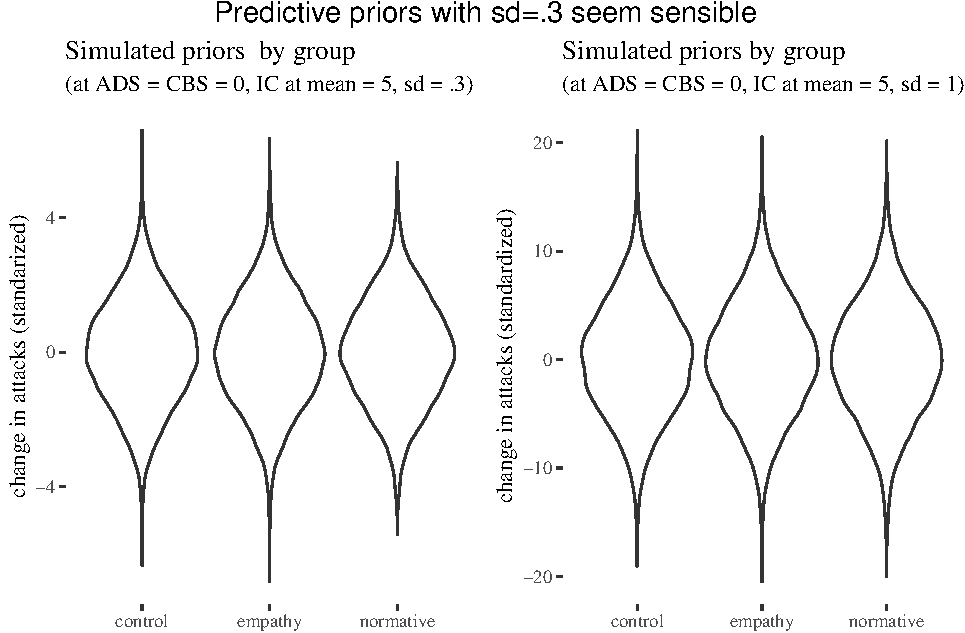
\includegraphics[width=1\linewidth]{bayesianReport3_files/figure-latex/priors03-1} \end{center}
\normalsize

Now, some model diagnostics before we move on. What we are witnessing is
(1) stationarity (the chains stay mostly in the most probable regions),
(2) good mixing (they explore a range of options in the beginning), and
(3) convergence (they stabilize as they progress).

\vspace{1mm}
\footnotesize

\begin{Shaded}
\begin{Highlighting}[]
\FunctionTok{traceplot}\NormalTok{( InteractionsModelDiff )}
\end{Highlighting}
\end{Shaded}

\begin{center}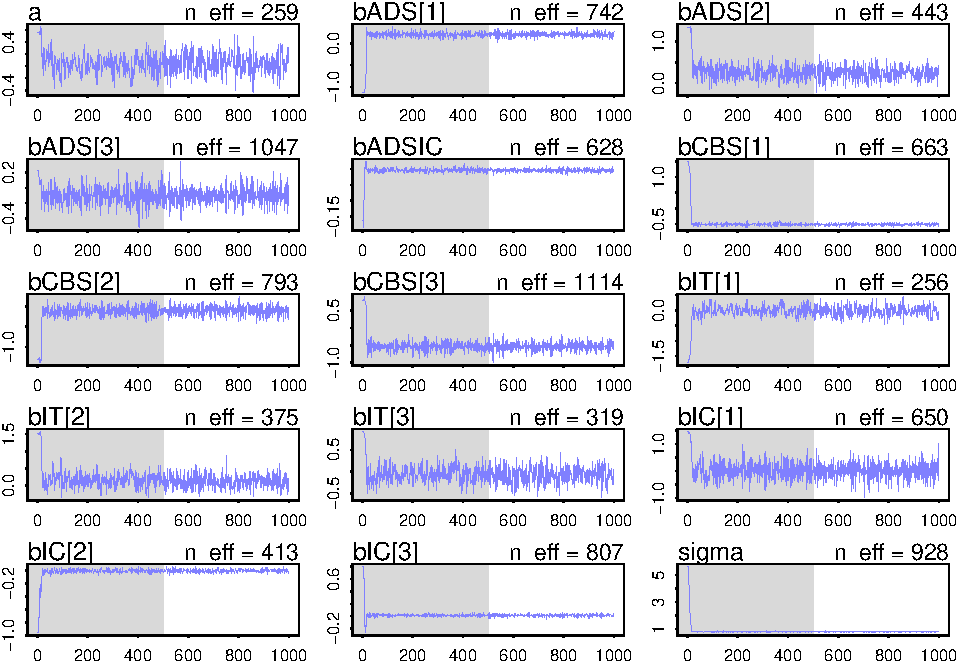
\includegraphics[width=1\linewidth]{bayesianReport3_files/figure-latex/unnamed-chunk-6-1} \end{center}
\normalsize

Finally, let's inspect the distribution of residuals. That is, we
calculate all predictions, their distance from the actual values, and
inspect the distribution of the distances:

\vspace{1mm}
\footnotesize

\begin{Shaded}
\begin{Highlighting}[]
\NormalTok{mu }\OtherTok{\textless{}{-}} \FunctionTok{link}\NormalTok{(InteractionsModelDiff)}
\NormalTok{mu\_mean }\OtherTok{\textless{}{-}} \FunctionTok{apply}\NormalTok{( mu , }\DecValTok{2}\NormalTok{ , mean )}
\NormalTok{mu\_resid }\OtherTok{\textless{}{-}}\NormalTok{ summaries}\SpecialCharTok{$}\NormalTok{AdiffS }\SpecialCharTok{{-}}\NormalTok{ mu\_mean}
\FunctionTok{ggplot}\NormalTok{()}\SpecialCharTok{+}\FunctionTok{geom\_density}\NormalTok{(}\FunctionTok{aes}\NormalTok{(}\AttributeTok{x =}\NormalTok{ mu\_resid))}\SpecialCharTok{+}\FunctionTok{theme\_tufte}\NormalTok{()}\SpecialCharTok{+}
  \FunctionTok{ggtitle}\NormalTok{(}\StringTok{"Residuals are approximately normally distributed"}\NormalTok{)}\SpecialCharTok{+}\FunctionTok{xlab}\NormalTok{(}\StringTok{"residuals"}\NormalTok{)}
\end{Highlighting}
\end{Shaded}

\begin{center}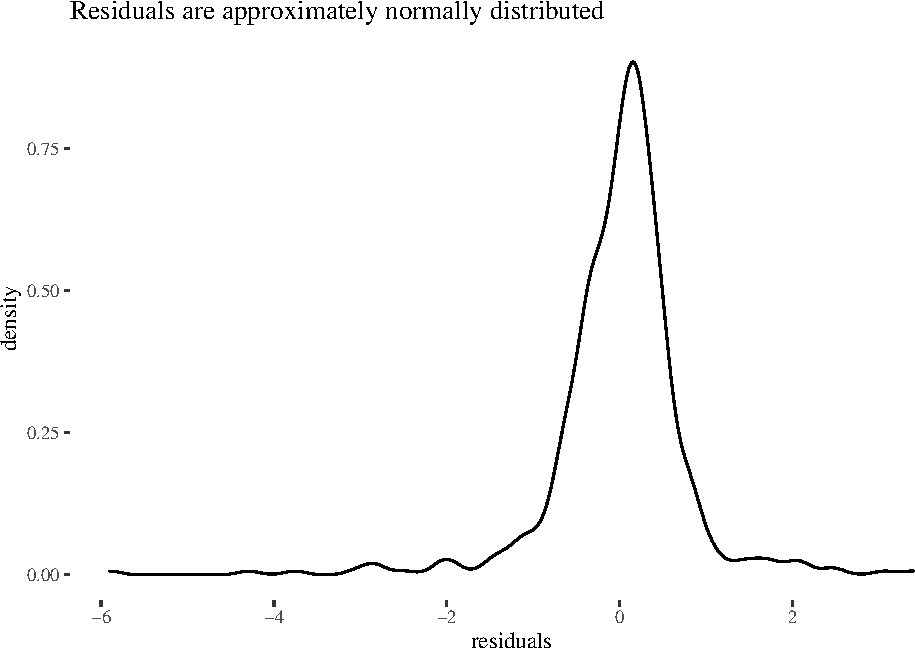
\includegraphics[width=1\linewidth]{bayesianReport3_files/figure-latex/unnamed-chunk-7-1} \end{center}
\normalsize

\hypertarget{model-selection}{%
\section{Model selection}\label{model-selection}}

How did we get to this fairly complicated model though? Once preliminary
causal considerations guided our restrictions on variable selection, we
proceed by building models of increasing complexity, and comparing them
in terms of Widely Acceptable Information Criterion. The models differ
mostly in the underlying linear formulae. For computational ease we will
here use quadratic approximations, while in the final analysis we will
deploy Hamiltionian Monte Carlo. The names are meant to decode the model
structure: the predictors are listed before dashes, whereas interactions
are listed after dashes.

\begin{align}
\tag{Null}  \mu_i & = \alpha\\
\tag{ADS}  \mu_i & = \alpha + \beta_{\mathsf{ADS}}\times \mathsf{ADS}\\
\tag{ADSIC}  \mu_i & = \alpha + \beta_{\mathsf{ADS}}\times \mathsf{ADS} +    \beta_{\mathsf{IC}}\times \mathsf{IC}\\
\tag{IT}  \mu_i & = \beta_{\mathsf{group}[i]} \\
\tag{ADSIT} \mu_i & = \alpha + \beta_{\mathsf{ADS}}\times \mathsf{ADS} +  \beta_{\mathsf{group}[i]}\\
\tag{ADSITIC} \mu_i & = \alpha + \beta_{\mathsf{ADS}}\times \mathsf{ADS} +  \beta_{\mathsf{group}[i]} +    \beta_{\mathsf{IC}}\times \mathsf{IC}\\
\tag{ADSITIC-ADSIC} \mu_i & = \alpha + \beta_{\mathsf{ADS}}\times \mathsf{ADS} +  \beta_{\mathsf{group}[i]} +    \beta_{\mathsf{IC}}\times \mathsf{IC} + \beta_{\mathsf{ADSIC}}\times \mathsf{ADS} \times \mathsf{IC}\\
\tag{ADSITIC-ADSIC-ADSIT} \mu_i & = \alpha + \beta_{\mathsf{ADS}}[\mathsf{group}_i]\times \mathsf{ADS} +  \beta_{\mathsf{group}[i]} +  \\ \nonumber & +  \beta_{\mathsf{IC}}\times \mathsf{IC} + \beta_{\mathsf{ADSIC}}\times \mathsf{ADS} \times \mathsf{IC}\\
\tag{ADSIT-ADSIT}   \mu_i &  = \alpha + \beta_{\mathsf{ADS}}[\mathsf{group}_i] \times
 \mathsf{ADS} + \beta_{\mathsf{group}[i]} \\
\tag{ADSITIC-ADSIT-ITIC-ADSIC}   \mu_i &  = \alpha  +  \beta_{\mathsf{ADS}}[\mathsf{group}_i] \times \mathsf{ADS} + \beta_{\mathsf{group}[i]} +  
\beta_{\mathsf{IC}}[\mathsf{group}_i] \times \mathsf{IC} + \\ \nonumber & + \beta_{\mathsf{ADSIC}}\times \mathsf{ADS} \times \mathsf{IC}\\
\tag{ADSITICCBS-ITIC-ADSIC} \mu_i &  = \alpha  +  \beta_{\mathsf{ADS}}[\mathsf{group}_i] \times
 \mathsf{ADS}  + \beta_{\mathsf{group}[i]} +   \beta_{\mathsf{IC}}[\mathsf{group}_i] \times \mathsf{IC} + \\ & \nonumber  + \beta_{\mathsf{CBS}} \times \mathsf{CBS} +  \beta_{\mathsf{ADSIC}}\times \mathsf{ADS} \times \mathsf{IC}  \\
\tag{Final} \mu_i & = \alpha + \beta_{\mathsf{ADS}}[\mathsf{group}_i]\times \mathsf{ADS} + \beta_{\mathsf{group}_i}  +  \beta_{\mathsf{IC}}[\mathsf{group}_i]\times \mathsf{IC} + \\
 & + \beta_{\mathsf{ADSIC}}\times \mathsf{ADS} \times \mathsf{IC} + \beta_{\mathsf{CBS}}[\mathsf{group}_i] \times \mathsf{CBS} \nonumber\\
 \tag{tooFAr} \mu_i & = \alpha + \beta_{\mathsf{ADS}}[\mathsf{group}_i]\times \mathsf{ADS} + \beta_{\mathsf{group}_i}  +  \beta_{\mathsf{IC}}[\mathsf{group}_i]\times \mathsf{IC} + \\
 & + \beta_{\mathsf{ADSIC}}\times \mathsf{ADS} \times \mathsf{IC} + \beta_{\mathsf{CBS}}[\mathsf{group}_i] \times \mathsf{CBS} + \beta_{\mathsf{CBSIC}}\times
 \mathsf{CBS} \times \mathsf{IC}\end{align}

\vspace{1mm}
\footnotesize

\begin{Shaded}
\begin{Highlighting}[]
\NormalTok{null }\OtherTok{\textless{}{-}} \FunctionTok{quap}\NormalTok{(}
  \FunctionTok{alist}\NormalTok{(}
\NormalTok{    AdiffS }\SpecialCharTok{\textasciitilde{}} \FunctionTok{dnorm}\NormalTok{( mu, sigma ),}
\NormalTok{    mu }\SpecialCharTok{\textasciitilde{}} \FunctionTok{dnorm}\NormalTok{ (}\DecValTok{0}\NormalTok{,}\FloatTok{0.3}\NormalTok{),}
\NormalTok{    sigma  }\SpecialCharTok{\textasciitilde{}} \FunctionTok{dexp}\NormalTok{(}\DecValTok{1}\NormalTok{)}
\NormalTok{  ), }
  \AttributeTok{data =}\NormalTok{ summaries  }
\NormalTok{)}

\NormalTok{ADS }\OtherTok{\textless{}{-}} \FunctionTok{quap}\NormalTok{(}
  \FunctionTok{alist}\NormalTok{(}
\NormalTok{    AdiffS }\SpecialCharTok{\textasciitilde{}} \FunctionTok{dnorm}\NormalTok{( mu, sigma ),}
\NormalTok{    mu }\OtherTok{\textless{}{-}}\NormalTok{  a }\SpecialCharTok{+}\NormalTok{ bADS }\SpecialCharTok{*}\NormalTok{ ADS,}
\NormalTok{    a }\SpecialCharTok{\textasciitilde{}} \FunctionTok{dnorm}\NormalTok{ (}\DecValTok{0}\NormalTok{,}\FloatTok{0.3}\NormalTok{),}
\NormalTok{    bADS }\SpecialCharTok{\textasciitilde{}} \FunctionTok{dnorm}\NormalTok{(}\DecValTok{0}\NormalTok{,}\FloatTok{0.3}\NormalTok{),}
\NormalTok{    sigma  }\SpecialCharTok{\textasciitilde{}} \FunctionTok{dexp}\NormalTok{(}\DecValTok{1}\NormalTok{)}
\NormalTok{  ), }
  \AttributeTok{data =}\NormalTok{ summaries}
\NormalTok{)}

\NormalTok{ADSIC }\OtherTok{\textless{}{-}} \FunctionTok{quap}\NormalTok{(}
  \FunctionTok{alist}\NormalTok{(}
\NormalTok{    AdiffS }\SpecialCharTok{\textasciitilde{}} \FunctionTok{dnorm}\NormalTok{( mu, sigma ),}
\NormalTok{    mu }\OtherTok{\textless{}{-}}\NormalTok{  a }\SpecialCharTok{+}\NormalTok{ bADS }\SpecialCharTok{*}\NormalTok{ ADS}\SpecialCharTok{+}\NormalTok{ bIC }\SpecialCharTok{*}\NormalTok{ IC,}
\NormalTok{    a }\SpecialCharTok{\textasciitilde{}} \FunctionTok{dnorm}\NormalTok{ (}\DecValTok{0}\NormalTok{,}\FloatTok{0.3}\NormalTok{),}
\NormalTok{    bADS }\SpecialCharTok{\textasciitilde{}} \FunctionTok{dnorm}\NormalTok{(}\DecValTok{0}\NormalTok{,}\FloatTok{0.3}\NormalTok{),}
\NormalTok{    bIC }\SpecialCharTok{\textasciitilde{}} \FunctionTok{dnorm}\NormalTok{(}\DecValTok{0}\NormalTok{,}\FloatTok{0.3}\NormalTok{),}
\NormalTok{    sigma  }\SpecialCharTok{\textasciitilde{}} \FunctionTok{dexp}\NormalTok{(}\DecValTok{1}\NormalTok{)}
\NormalTok{  ), }
  \AttributeTok{data =}\NormalTok{ summaries}
\NormalTok{)}


\NormalTok{IT }\OtherTok{\textless{}{-}} \FunctionTok{quap}\NormalTok{(}
  \FunctionTok{alist}\NormalTok{(}
\NormalTok{    AdiffS }\SpecialCharTok{\textasciitilde{}} \FunctionTok{dnorm}\NormalTok{( mu, sigma ),}
\NormalTok{    mu }\OtherTok{\textless{}{-}}\NormalTok{  bIT[groupID] ,}
\NormalTok{    bIT[groupID] }\SpecialCharTok{\textasciitilde{}} \FunctionTok{dnorm}\NormalTok{(}\DecValTok{0}\NormalTok{,.}\DecValTok{3}\NormalTok{),}
\NormalTok{    sigma  }\SpecialCharTok{\textasciitilde{}} \FunctionTok{dexp}\NormalTok{(}\DecValTok{1}\NormalTok{)}
\NormalTok{  ), }
  \AttributeTok{data =}\NormalTok{ summaries}
\NormalTok{)}


\NormalTok{ADSIT }\OtherTok{\textless{}{-}} \FunctionTok{quap}\NormalTok{(}
  \FunctionTok{alist}\NormalTok{(}
\NormalTok{    AdiffS }\SpecialCharTok{\textasciitilde{}} \FunctionTok{dnorm}\NormalTok{( mu, sigma ),}
\NormalTok{    mu }\OtherTok{\textless{}{-}}\NormalTok{ a }\SpecialCharTok{+}\NormalTok{ bADS }\SpecialCharTok{*}\NormalTok{ ADS }\SpecialCharTok{+}\NormalTok{  bIT[groupID],}
\NormalTok{    a }\SpecialCharTok{\textasciitilde{}} \FunctionTok{dnorm}\NormalTok{ (}\DecValTok{0}\NormalTok{,}\FloatTok{0.3}\NormalTok{),}
\NormalTok{    bADS }\SpecialCharTok{\textasciitilde{}} \FunctionTok{dnorm}\NormalTok{(}\DecValTok{0}\NormalTok{,.}\DecValTok{3}\NormalTok{),}
\NormalTok{    bIT[groupID] }\SpecialCharTok{\textasciitilde{}} \FunctionTok{dnorm}\NormalTok{(}\DecValTok{0}\NormalTok{,.}\DecValTok{3}\NormalTok{),}
\NormalTok{    sigma  }\SpecialCharTok{\textasciitilde{}} \FunctionTok{dexp}\NormalTok{(}\DecValTok{1}\NormalTok{)}
\NormalTok{  ), }
  \AttributeTok{data =}\NormalTok{ summaries}
\NormalTok{)}


\NormalTok{ADSITIC }\OtherTok{\textless{}{-}} \FunctionTok{quap}\NormalTok{(}
  \FunctionTok{alist}\NormalTok{(}
\NormalTok{    AdiffS }\SpecialCharTok{\textasciitilde{}} \FunctionTok{dnorm}\NormalTok{( mu, sigma ),}
\NormalTok{    mu }\OtherTok{\textless{}{-}}\NormalTok{ a }\SpecialCharTok{+}\NormalTok{ bADS }\SpecialCharTok{*}\NormalTok{ ADS }\SpecialCharTok{+}\NormalTok{  bIT[groupID] }\SpecialCharTok{+}\NormalTok{ bIC }\SpecialCharTok{*}\NormalTok{ IC,}
\NormalTok{    a }\SpecialCharTok{\textasciitilde{}} \FunctionTok{dnorm}\NormalTok{ (}\DecValTok{0}\NormalTok{,}\FloatTok{0.3}\NormalTok{),}
\NormalTok{    bADS }\SpecialCharTok{\textasciitilde{}} \FunctionTok{dnorm}\NormalTok{(}\DecValTok{0}\NormalTok{,.}\DecValTok{3}\NormalTok{),}
\NormalTok{    bIT[groupID] }\SpecialCharTok{\textasciitilde{}} \FunctionTok{dnorm}\NormalTok{(}\DecValTok{0}\NormalTok{,.}\DecValTok{3}\NormalTok{),}
\NormalTok{    bIC }\SpecialCharTok{\textasciitilde{}} \FunctionTok{dnorm}\NormalTok{(}\DecValTok{0}\NormalTok{,.}\DecValTok{3}\NormalTok{),}
\NormalTok{    sigma  }\SpecialCharTok{\textasciitilde{}} \FunctionTok{dexp}\NormalTok{(}\DecValTok{1}\NormalTok{)}
\NormalTok{  ), }
  \AttributeTok{data =}\NormalTok{ summaries}
\NormalTok{)}


\NormalTok{ADSITIC\_ADSIC }\OtherTok{\textless{}{-}} \FunctionTok{quap}\NormalTok{(}
  \FunctionTok{alist}\NormalTok{(}
\NormalTok{    AdiffS }\SpecialCharTok{\textasciitilde{}} \FunctionTok{dnorm}\NormalTok{( mu, sigma ),}
\NormalTok{    mu }\OtherTok{\textless{}{-}}\NormalTok{ a }\SpecialCharTok{+}\NormalTok{ bADS }\SpecialCharTok{*}\NormalTok{ ADS }\SpecialCharTok{+}\NormalTok{  bIT[groupID] }\SpecialCharTok{+}\NormalTok{ bIC }\SpecialCharTok{*}\NormalTok{ IC }\SpecialCharTok{+}\NormalTok{ bADSIC }\SpecialCharTok{*}\NormalTok{ ADS }\SpecialCharTok{*}\NormalTok{ IC,}
\NormalTok{    a }\SpecialCharTok{\textasciitilde{}} \FunctionTok{dnorm}\NormalTok{ (}\DecValTok{0}\NormalTok{,}\FloatTok{0.3}\NormalTok{),}
\NormalTok{    bADS }\SpecialCharTok{\textasciitilde{}} \FunctionTok{dnorm}\NormalTok{(}\DecValTok{0}\NormalTok{,.}\DecValTok{3}\NormalTok{),}
\NormalTok{    bADSIC }\SpecialCharTok{\textasciitilde{}} \FunctionTok{dnorm}\NormalTok{(}\DecValTok{0}\NormalTok{,.}\DecValTok{3}\NormalTok{),}
\NormalTok{    bIT[groupID] }\SpecialCharTok{\textasciitilde{}} \FunctionTok{dnorm}\NormalTok{(}\DecValTok{0}\NormalTok{,.}\DecValTok{3}\NormalTok{),}
\NormalTok{    bIC }\SpecialCharTok{\textasciitilde{}} \FunctionTok{dnorm}\NormalTok{(}\DecValTok{0}\NormalTok{,.}\DecValTok{3}\NormalTok{),}
\NormalTok{    sigma  }\SpecialCharTok{\textasciitilde{}} \FunctionTok{dexp}\NormalTok{(}\DecValTok{1}\NormalTok{)}
\NormalTok{  ), }
  \AttributeTok{data =}\NormalTok{ summaries}
\NormalTok{)}


\NormalTok{ADSITIC\_ADSIC\_ADSIT }\OtherTok{\textless{}{-}} \FunctionTok{quap}\NormalTok{(}
  \FunctionTok{alist}\NormalTok{(}
\NormalTok{    AdiffS }\SpecialCharTok{\textasciitilde{}} \FunctionTok{dnorm}\NormalTok{( mu, sigma ),}
\NormalTok{    mu }\OtherTok{\textless{}{-}}\NormalTok{ a }\SpecialCharTok{+}\NormalTok{ bADS[groupID] }\SpecialCharTok{*}\NormalTok{ ADS }\SpecialCharTok{+}\NormalTok{  bIT[groupID] }\SpecialCharTok{+}\NormalTok{ bIC }\SpecialCharTok{*}\NormalTok{ IC }\SpecialCharTok{+}\NormalTok{ bADSIC }\SpecialCharTok{*}\NormalTok{ ADS }\SpecialCharTok{*}\NormalTok{ IC,}
\NormalTok{    a }\SpecialCharTok{\textasciitilde{}} \FunctionTok{dnorm}\NormalTok{ (}\DecValTok{0}\NormalTok{,}\FloatTok{0.3}\NormalTok{),}
\NormalTok{    bADS[groupID] }\SpecialCharTok{\textasciitilde{}} \FunctionTok{dnorm}\NormalTok{(}\DecValTok{0}\NormalTok{,.}\DecValTok{3}\NormalTok{),}
\NormalTok{    bADSIC }\SpecialCharTok{\textasciitilde{}} \FunctionTok{dnorm}\NormalTok{(}\DecValTok{0}\NormalTok{,.}\DecValTok{3}\NormalTok{),}
\NormalTok{    bIT[groupID] }\SpecialCharTok{\textasciitilde{}} \FunctionTok{dnorm}\NormalTok{(}\DecValTok{0}\NormalTok{,.}\DecValTok{3}\NormalTok{),}
\NormalTok{    bIC }\SpecialCharTok{\textasciitilde{}} \FunctionTok{dnorm}\NormalTok{(}\DecValTok{0}\NormalTok{,.}\DecValTok{3}\NormalTok{),}
\NormalTok{    sigma  }\SpecialCharTok{\textasciitilde{}} \FunctionTok{dexp}\NormalTok{(}\DecValTok{1}\NormalTok{)}
\NormalTok{  ), }
  \AttributeTok{data =}\NormalTok{ summaries}
\NormalTok{)}


\NormalTok{ADSIT\_ADSIT }\OtherTok{\textless{}{-}} \FunctionTok{quap}\NormalTok{(}
  \FunctionTok{alist}\NormalTok{(}
\NormalTok{    AdiffS }\SpecialCharTok{\textasciitilde{}} \FunctionTok{dnorm}\NormalTok{( mu, sigma ),}
\NormalTok{    mu }\OtherTok{\textless{}{-}}\NormalTok{ a }\SpecialCharTok{+}\NormalTok{ bADS[groupID] }\SpecialCharTok{*}\NormalTok{ ADS }\SpecialCharTok{+}\NormalTok{  bIT[groupID] ,}
\NormalTok{    a }\SpecialCharTok{\textasciitilde{}} \FunctionTok{dnorm}\NormalTok{ (}\DecValTok{0}\NormalTok{,}\FloatTok{0.3}\NormalTok{),}
\NormalTok{    bADS[groupID] }\SpecialCharTok{\textasciitilde{}} \FunctionTok{dnorm}\NormalTok{(}\DecValTok{0}\NormalTok{,.}\DecValTok{3}\NormalTok{),}
    \CommentTok{\#bADSIC \textasciitilde{} dnorm(0,.5),}
\NormalTok{    bIT[groupID] }\SpecialCharTok{\textasciitilde{}} \FunctionTok{dnorm}\NormalTok{(}\DecValTok{0}\NormalTok{,.}\DecValTok{3}\NormalTok{),}
    \CommentTok{\#bIC \textasciitilde{} dnorm(0,.5),}
\NormalTok{    sigma  }\SpecialCharTok{\textasciitilde{}} \FunctionTok{dexp}\NormalTok{(}\DecValTok{1}\NormalTok{)}
\NormalTok{  ), }
  \AttributeTok{data =}\NormalTok{ summaries}
\NormalTok{)}


\NormalTok{ADSITIC\_ADSIT\_ITIC\_ADSIC }\OtherTok{\textless{}{-}} \FunctionTok{quap}\NormalTok{(}
  \FunctionTok{alist}\NormalTok{(}
\NormalTok{    AdiffS }\SpecialCharTok{\textasciitilde{}} \FunctionTok{dnorm}\NormalTok{( mu, sigma ),}
\NormalTok{    mu }\OtherTok{\textless{}{-}}\NormalTok{ a }\SpecialCharTok{+}\NormalTok{ bADS[groupID] }\SpecialCharTok{*}\NormalTok{ ADS }\SpecialCharTok{+}\NormalTok{  bIT[groupID] }\SpecialCharTok{+}\NormalTok{ bIC[groupID] }\SpecialCharTok{*}\NormalTok{ IC }\SpecialCharTok{+}
\NormalTok{      bADSIC }\SpecialCharTok{*}\NormalTok{ ADS }\SpecialCharTok{*}\NormalTok{ IC,}
\NormalTok{    a }\SpecialCharTok{\textasciitilde{}} \FunctionTok{dnorm}\NormalTok{ (}\DecValTok{0}\NormalTok{,}\FloatTok{0.3}\NormalTok{),}
\NormalTok{    bADS[groupID] }\SpecialCharTok{\textasciitilde{}} \FunctionTok{dnorm}\NormalTok{(}\DecValTok{0}\NormalTok{,.}\DecValTok{3}\NormalTok{),}
\NormalTok{    bADSIC }\SpecialCharTok{\textasciitilde{}} \FunctionTok{dnorm}\NormalTok{(}\DecValTok{0}\NormalTok{,.}\DecValTok{3}\NormalTok{),}
\NormalTok{    bIT[groupID] }\SpecialCharTok{\textasciitilde{}} \FunctionTok{dnorm}\NormalTok{(}\DecValTok{0}\NormalTok{,.}\DecValTok{3}\NormalTok{),}
\NormalTok{    bIC[groupID] }\SpecialCharTok{\textasciitilde{}} \FunctionTok{dnorm}\NormalTok{(}\DecValTok{0}\NormalTok{,.}\DecValTok{3}\NormalTok{),}
\NormalTok{    sigma  }\SpecialCharTok{\textasciitilde{}} \FunctionTok{dexp}\NormalTok{(}\DecValTok{1}\NormalTok{)}
\NormalTok{  ), }
  \AttributeTok{data =}\NormalTok{ summaries}
\NormalTok{)}


\NormalTok{ADSITICCBS\_ITIC\_ADSIC }\OtherTok{\textless{}{-}} \FunctionTok{quap}\NormalTok{(}
  \FunctionTok{alist}\NormalTok{(}
\NormalTok{    AdiffS }\SpecialCharTok{\textasciitilde{}} \FunctionTok{dnorm}\NormalTok{( mu, sigma ),}
\NormalTok{    mu }\OtherTok{\textless{}{-}}\NormalTok{ a }\SpecialCharTok{+}\NormalTok{ bADS[groupID] }\SpecialCharTok{*}\NormalTok{ ADS }\SpecialCharTok{+}\NormalTok{  bIT[groupID] }\SpecialCharTok{+}\NormalTok{ bIC[groupID] }\SpecialCharTok{*}\NormalTok{ IC }\SpecialCharTok{+} 
\NormalTok{      bADSIC }\SpecialCharTok{*}\NormalTok{ ADS }\SpecialCharTok{*}\NormalTok{ IC}\SpecialCharTok{+}\NormalTok{ bCBS }\SpecialCharTok{*}\NormalTok{CBS,}
\NormalTok{    a }\SpecialCharTok{\textasciitilde{}} \FunctionTok{dnorm}\NormalTok{ (}\DecValTok{0}\NormalTok{,}\FloatTok{0.3}\NormalTok{),}
\NormalTok{    bADS[groupID] }\SpecialCharTok{\textasciitilde{}} \FunctionTok{dnorm}\NormalTok{(}\DecValTok{0}\NormalTok{,.}\DecValTok{3}\NormalTok{),}
\NormalTok{    bADSIC }\SpecialCharTok{\textasciitilde{}} \FunctionTok{dnorm}\NormalTok{(}\DecValTok{0}\NormalTok{,.}\DecValTok{3}\NormalTok{),}
\NormalTok{    bCBS }\SpecialCharTok{\textasciitilde{}} \FunctionTok{dnorm}\NormalTok{(}\DecValTok{0}\NormalTok{,.}\DecValTok{3}\NormalTok{),}
\NormalTok{    bIT[groupID] }\SpecialCharTok{\textasciitilde{}} \FunctionTok{dnorm}\NormalTok{(}\DecValTok{0}\NormalTok{,.}\DecValTok{3}\NormalTok{),}
\NormalTok{    bIC[groupID] }\SpecialCharTok{\textasciitilde{}} \FunctionTok{dnorm}\NormalTok{(}\DecValTok{0}\NormalTok{,.}\DecValTok{3}\NormalTok{),}
\NormalTok{    sigma  }\SpecialCharTok{\textasciitilde{}} \FunctionTok{dexp}\NormalTok{(}\DecValTok{1}\NormalTok{)}
\NormalTok{  ), }
  \AttributeTok{data =}\NormalTok{ summaries}
\NormalTok{)}


\NormalTok{Final }\OtherTok{\textless{}{-}} \FunctionTok{quap}\NormalTok{(}
  \FunctionTok{alist}\NormalTok{(}
\NormalTok{    AdiffS }\SpecialCharTok{\textasciitilde{}} \FunctionTok{dnorm}\NormalTok{( mu, sigma ),}
\NormalTok{    mu }\OtherTok{\textless{}{-}}\NormalTok{ a }\SpecialCharTok{+}\NormalTok{ bADS[groupID] }\SpecialCharTok{*}\NormalTok{ ADS }\SpecialCharTok{+}\NormalTok{  bIT[groupID] }\SpecialCharTok{+}\NormalTok{ bIC[groupID] }\SpecialCharTok{*}\NormalTok{ IC }\SpecialCharTok{+} 
\NormalTok{      bADSIC }\SpecialCharTok{*}\NormalTok{ ADS }\SpecialCharTok{*}\NormalTok{ IC}\SpecialCharTok{+}\NormalTok{ bCBS[groupID] }\SpecialCharTok{*}\NormalTok{CBS,}
\NormalTok{    a }\SpecialCharTok{\textasciitilde{}} \FunctionTok{dnorm}\NormalTok{ (}\DecValTok{0}\NormalTok{,}\FloatTok{0.3}\NormalTok{),}
\NormalTok{    bADS[groupID] }\SpecialCharTok{\textasciitilde{}} \FunctionTok{dnorm}\NormalTok{(}\DecValTok{0}\NormalTok{,.}\DecValTok{3}\NormalTok{),}
\NormalTok{    bADSIC }\SpecialCharTok{\textasciitilde{}} \FunctionTok{dnorm}\NormalTok{(}\DecValTok{0}\NormalTok{,.}\DecValTok{3}\NormalTok{),}
\NormalTok{    bCBS[groupID] }\SpecialCharTok{\textasciitilde{}} \FunctionTok{dnorm}\NormalTok{(}\DecValTok{0}\NormalTok{,.}\DecValTok{3}\NormalTok{),}
\NormalTok{    bIT[groupID] }\SpecialCharTok{\textasciitilde{}} \FunctionTok{dnorm}\NormalTok{(}\DecValTok{0}\NormalTok{,.}\DecValTok{3}\NormalTok{),}
\NormalTok{    bIC[groupID] }\SpecialCharTok{\textasciitilde{}} \FunctionTok{dnorm}\NormalTok{(}\DecValTok{0}\NormalTok{,.}\DecValTok{3}\NormalTok{),}
\NormalTok{    sigma  }\SpecialCharTok{\textasciitilde{}} \FunctionTok{dexp}\NormalTok{(}\DecValTok{1}\NormalTok{)}
\NormalTok{  ), }
  \AttributeTok{data =}\NormalTok{ summaries}
\NormalTok{)}



\NormalTok{tooFar }\OtherTok{\textless{}{-}} \FunctionTok{quap}\NormalTok{(}
  \FunctionTok{alist}\NormalTok{(}
\NormalTok{    AdiffS }\SpecialCharTok{\textasciitilde{}} \FunctionTok{dnorm}\NormalTok{( mu, sigma ),}
\NormalTok{    mu }\OtherTok{\textless{}{-}}\NormalTok{ a }\SpecialCharTok{+}\NormalTok{ bADS[groupID] }\SpecialCharTok{*}\NormalTok{ ADS }\SpecialCharTok{+}\NormalTok{  bIT[groupID] }\SpecialCharTok{+}\NormalTok{ bIC[groupID] }\SpecialCharTok{*}\NormalTok{ IC }\SpecialCharTok{+} 
\NormalTok{      bADSIC }\SpecialCharTok{*}\NormalTok{ ADS }\SpecialCharTok{*}\NormalTok{ IC}\SpecialCharTok{+}\NormalTok{ bCBS[groupID] }\SpecialCharTok{*}\NormalTok{CBS }\SpecialCharTok{+}\NormalTok{ bCBSIC }\SpecialCharTok{*}\NormalTok{ CBS }\SpecialCharTok{*}\NormalTok{ IC, }
\NormalTok{    a }\SpecialCharTok{\textasciitilde{}} \FunctionTok{dnorm}\NormalTok{ (}\DecValTok{0}\NormalTok{,}\FloatTok{0.3}\NormalTok{),}
\NormalTok{    bADS[groupID] }\SpecialCharTok{\textasciitilde{}} \FunctionTok{dnorm}\NormalTok{(}\DecValTok{0}\NormalTok{,.}\DecValTok{3}\NormalTok{),}
\NormalTok{    bADSIC }\SpecialCharTok{\textasciitilde{}} \FunctionTok{dnorm}\NormalTok{(}\DecValTok{0}\NormalTok{,.}\DecValTok{3}\NormalTok{),}
\NormalTok{    bCBS[groupID] }\SpecialCharTok{\textasciitilde{}} \FunctionTok{dnorm}\NormalTok{(}\DecValTok{0}\NormalTok{,.}\DecValTok{3}\NormalTok{),}
\NormalTok{    bIT[groupID] }\SpecialCharTok{\textasciitilde{}} \FunctionTok{dnorm}\NormalTok{(}\DecValTok{0}\NormalTok{,.}\DecValTok{3}\NormalTok{),}
\NormalTok{    bIC[groupID] }\SpecialCharTok{\textasciitilde{}} \FunctionTok{dnorm}\NormalTok{(}\DecValTok{0}\NormalTok{,.}\DecValTok{3}\NormalTok{),}
\NormalTok{     bCBSIC }\SpecialCharTok{\textasciitilde{}} \FunctionTok{dnorm}\NormalTok{(}\DecValTok{0}\NormalTok{, .}\DecValTok{3}\NormalTok{),}
\NormalTok{    sigma  }\SpecialCharTok{\textasciitilde{}} \FunctionTok{dexp}\NormalTok{(}\DecValTok{1}\NormalTok{)}
\NormalTok{  ), }
  \AttributeTok{data =}\NormalTok{ summaries}
\NormalTok{)}
\end{Highlighting}
\end{Shaded}

\normalsize

\vspace{1mm}
\footnotesize

\begin{Shaded}
\begin{Highlighting}[]
\NormalTok{comparison}\OtherTok{\textless{}{-}} \FunctionTok{compare}\NormalTok{(null,ADS,ADSIC,IT,ADSIT,ADSITIC,ADSITIC\_ADSIC,}
\NormalTok{                     ADSITIC\_ADSIC\_ADSIT,ADSIT\_ADSIT,ADSITIC\_ADSIT\_ITIC\_ADSIC,}
\NormalTok{                     ADSITICCBS\_ITIC\_ADSIC,Final, tooFar)}
\FunctionTok{mykable}\NormalTok{(}\FunctionTok{round}\NormalTok{(}\FunctionTok{data.frame}\NormalTok{(comparison ),}\DecValTok{3}\NormalTok{)) }
\end{Highlighting}
\end{Shaded}

\begin{table}
\centering\begingroup\fontsize{9}{11}\selectfont

\begin{tabular}{lrrrrrr}
\toprule
  & WAIC & SE & dWAIC & dSE & pWAIC & weight\\
\midrule
\cellcolor{gray!6}{tooFar} & \cellcolor{gray!6}{1185.575} & \cellcolor{gray!6}{89.393} & \cellcolor{gray!6}{0.000} & \cellcolor{gray!6}{NA} & \cellcolor{gray!6}{27.846} & \cellcolor{gray!6}{0.487}\\
Final & 1185.657 & 89.827 & 0.082 & 2.594 & 27.614 & 0.467\\
\cellcolor{gray!6}{ADSITICCBS\_ITIC\_ADSIC} & \cellcolor{gray!6}{1190.304} & \cellcolor{gray!6}{87.920} & \cellcolor{gray!6}{4.729} & \cellcolor{gray!6}{6.055} & \cellcolor{gray!6}{25.882} & \cellcolor{gray!6}{0.046}\\
null & 1345.358 & 145.805 & 159.783 & 134.039 & 18.061 & 0.000\\
\cellcolor{gray!6}{ADS} & \cellcolor{gray!6}{1347.281} & \cellcolor{gray!6}{142.655} & \cellcolor{gray!6}{161.706} & \cellcolor{gray!6}{131.261} & \cellcolor{gray!6}{21.935} & \cellcolor{gray!6}{0.000}\\
\addlinespace
IT & 1347.916 & 146.200 & 162.341 & 134.462 & 20.545 & 0.000\\
\cellcolor{gray!6}{ADSITIC\_ADSIC} & \cellcolor{gray!6}{1348.366} & \cellcolor{gray!6}{150.638} & \cellcolor{gray!6}{162.791} & \cellcolor{gray!6}{136.811} & \cellcolor{gray!6}{27.604} & \cellcolor{gray!6}{0.000}\\
ADSIT & 1350.067 & 144.264 & 164.492 & 132.764 & 23.985 & 0.000\\
\cellcolor{gray!6}{ADSIT\_ADSIT} & \cellcolor{gray!6}{1351.139} & \cellcolor{gray!6}{154.826} & \cellcolor{gray!6}{165.564} & \cellcolor{gray!6}{141.033} & \cellcolor{gray!6}{31.062} & \cellcolor{gray!6}{0.000}\\
ADSIC & 1351.343 & 145.539 & 165.768 & 133.454 & 25.443 & 0.000\\
\addlinespace
\cellcolor{gray!6}{ADSITIC} & \cellcolor{gray!6}{1353.020} & \cellcolor{gray!6}{147.645} & \cellcolor{gray!6}{167.445} & \cellcolor{gray!6}{135.441} & \cellcolor{gray!6}{26.884} & \cellcolor{gray!6}{0.000}\\
ADSITIC\_ADSIT\_ITIC\_ADSIC & 1355.187 & 154.826 & 169.613 & 140.659 & 34.652 & 0.000\\
\cellcolor{gray!6}{ADSITIC\_ADSIC\_ADSIT} & \cellcolor{gray!6}{1356.479} & \cellcolor{gray!6}{157.522} & \cellcolor{gray!6}{170.905} & \cellcolor{gray!6}{143.538} & \cellcolor{gray!6}{34.533} & \cellcolor{gray!6}{0.000}\\
\bottomrule
\end{tabular}
\endgroup{}
\end{table}

\begin{Shaded}
\begin{Highlighting}[]
\FunctionTok{plot}\NormalTok{(comparison)}
\end{Highlighting}
\end{Shaded}

\begin{center}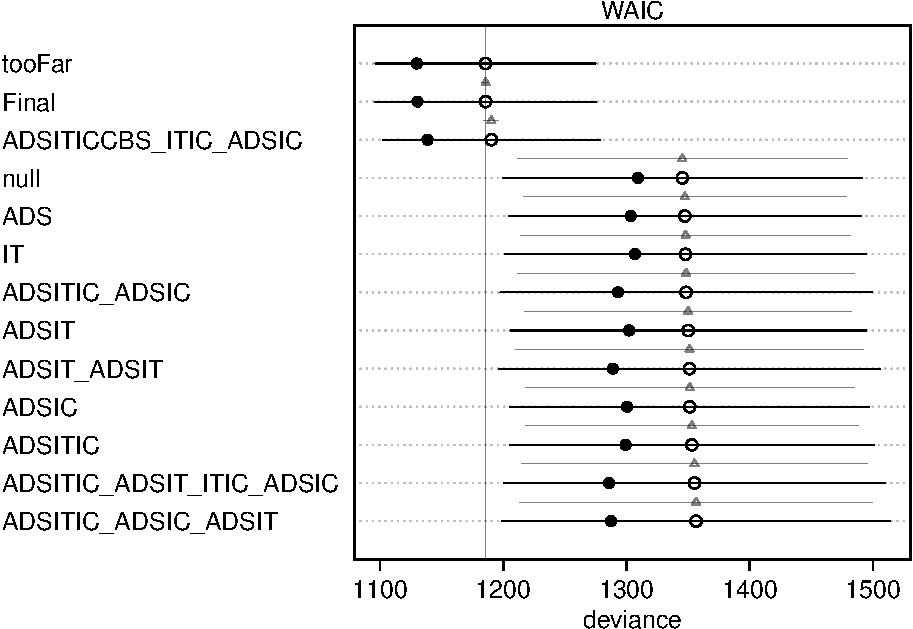
\includegraphics[width=1\linewidth]{bayesianReport3_files/figure-latex/unnamed-chunk-9-1} \end{center}
\normalsize

The three models that stand out differ in including \(\mathsf{CBS}\) as
a predictor. Moreover the final model includes an interaction between
treatment group and \(\mathsf{CBS}\). Adding a further interaction
between \(\mathsf{CBS}\) and \(\mathsf{IC}\) takes us too far.
\(WAIC\)-based weighing assigns the weight of \(83\%\) to the final
model, and the standard errors for the difference in WAIC for the top
three models is fairly low, so we will employ the top model
(\(\mathsf{Final}\)) in further analyses.

\hypertarget{inspecting-the-model-and-effect-sizes}{%
\section{Inspecting the model and effect
sizes}\label{inspecting-the-model-and-effect-sizes}}

We start by using the \textsf{Final} model formula to build a model,
this time using Hamiltionian Monte Carlo. We leave the code commented
out and load a pre-compiled model for computational convenience

\vspace{1mm}
\footnotesize

\begin{Shaded}
\begin{Highlighting}[]
\CommentTok{\# FinalHMC \textless{}{-} ulam(}
\CommentTok{\#   alist(}
\CommentTok{\#     AdiffS \textasciitilde{} dnorm( mu, sigma ),}
\CommentTok{\#     mu \textless{}{-} a + bADS[groupID] * ADS +  bIT[groupID] +}
\CommentTok{\#     bIC[groupID] * IC + bADSIC * ADS * IC+}
\CommentTok{\#     bCBS[groupID] *CBS,}
\CommentTok{\#     a \textasciitilde{} dnorm (0,0.3),}
\CommentTok{\#     bADS[groupID] \textasciitilde{} dnorm(0,.3),}
\CommentTok{\#     bADSIC \textasciitilde{} dnorm(0,.3),}
\CommentTok{\#     bCBS[groupID] \textasciitilde{} dnorm(0,.3),}
\CommentTok{\#     bIT[groupID] \textasciitilde{} dnorm(0,.3),}
\CommentTok{\#     bIC[groupID] \textasciitilde{} dnorm(0,.3),}
\CommentTok{\#     sigma  \textasciitilde{} dexp(1)}
\CommentTok{\#   ),}
\CommentTok{\#   data = summaries}
\CommentTok{\# )}
\CommentTok{\# saveRDS(FinalHMC, file = "models/FinalHMC.rds")}


\CommentTok{\#saveRDS(FinalHMC, file = "models/FinalHMC.rds")}

\NormalTok{FinalHMC }\OtherTok{\textless{}{-}} \FunctionTok{readRDS}\NormalTok{(}\AttributeTok{file =} \StringTok{"models/FinalHMC.rds"}\NormalTok{)}
\end{Highlighting}
\end{Shaded}

\normalsize

First, let's take a look at the best model coefficients.

\vspace{1mm}
\footnotesize

\begin{Shaded}
\begin{Highlighting}[]
\FunctionTok{mykable}\NormalTok{(}\FunctionTok{data.frame}\NormalTok{(}\FunctionTok{precis}\NormalTok{(FinalHMC, }\AttributeTok{depth =} \DecValTok{2}\NormalTok{)))}
\end{Highlighting}
\end{Shaded}

\begin{table}
\centering\begingroup\fontsize{9}{11}\selectfont

\begin{tabular}{lrrrrrr}
\toprule
  & mean & sd & X5.5. & X94.5. & n\_eff & Rhat4\\
\midrule
\cellcolor{gray!6}{a} & \cellcolor{gray!6}{0.0414089} & \cellcolor{gray!6}{0.1562753} & \cellcolor{gray!6}{-0.2037740} & \cellcolor{gray!6}{0.2796946} & \cellcolor{gray!6}{228.1593} & \cellcolor{gray!6}{0.9980513}\\
bADS[1] & 0.1979211 & 0.0568494 & 0.1086423 & 0.2907669 & 768.4216 & 1.0013137\\
\cellcolor{gray!6}{bADS[2]} & \cellcolor{gray!6}{0.2484756} & \cellcolor{gray!6}{0.1546028} & \cellcolor{gray!6}{0.0036955} & \cellcolor{gray!6}{0.4942282} & \cellcolor{gray!6}{526.1494} & \cellcolor{gray!6}{0.9995921}\\
bADS[3] & -0.1097667 & 0.1014546 & -0.2678764 & 0.0628934 & 418.0876 & 0.9980791\\
\cellcolor{gray!6}{bADSIC} & \cellcolor{gray!6}{-0.0042060} & \cellcolor{gray!6}{0.0051643} & \cellcolor{gray!6}{-0.0122338} & \cellcolor{gray!6}{0.0040408} & \cellcolor{gray!6}{361.1195} & \cellcolor{gray!6}{0.9983620}\\
\addlinespace
bCBS[1] & -0.5142899 & 0.0414267 & -0.5776731 & -0.4463925 & 722.3116 & 0.9991926\\
\cellcolor{gray!6}{bCBS[2]} & \cellcolor{gray!6}{-0.0919148} & \cellcolor{gray!6}{0.1245614} & \cellcolor{gray!6}{-0.2965873} & \cellcolor{gray!6}{0.1059034} & \cellcolor{gray!6}{671.6673} & \cellcolor{gray!6}{0.9998084}\\
bCBS[3] & -0.5302840 & 0.1088835 & -0.7023272 & -0.3593766 & 823.7157 & 0.9980583\\
\cellcolor{gray!6}{bIT[1]} & \cellcolor{gray!6}{-0.0212337} & \cellcolor{gray!6}{0.1630179} & \cellcolor{gray!6}{-0.2603815} & \cellcolor{gray!6}{0.2295494} & \cellcolor{gray!6}{219.0190} & \cellcolor{gray!6}{0.9980137}\\
bIT[2] & 0.1482970 & 0.1857528 & -0.1246834 & 0.4367149 & 304.7859 & 0.9980345\\
\addlinespace
\cellcolor{gray!6}{bIT[3]} & \cellcolor{gray!6}{-0.0686005} & \cellcolor{gray!6}{0.1776783} & \cellcolor{gray!6}{-0.3448157} & \cellcolor{gray!6}{0.2099344} & \cellcolor{gray!6}{295.3412} & \cellcolor{gray!6}{0.9980482}\\
bIC[1] & -0.0037630 & 0.3161707 & -0.5084313 & 0.4981378 & 829.2326 & 1.0011451\\
\cellcolor{gray!6}{bIC[2]} & \cellcolor{gray!6}{-0.0117801} & \cellcolor{gray!6}{0.0256771} & \cellcolor{gray!6}{-0.0529960} & \cellcolor{gray!6}{0.0290304} & \cellcolor{gray!6}{488.1809} & \cellcolor{gray!6}{0.9994090}\\
bIC[3] & 0.0118155 & 0.0185521 & -0.0192521 & 0.0412303 & 612.3810 & 0.9986804\\
\cellcolor{gray!6}{sigma} & \cellcolor{gray!6}{0.7945882} & \cellcolor{gray!6}{0.0277774} & \cellcolor{gray!6}{0.7535960} & \cellcolor{gray!6}{0.8434971} & \cellcolor{gray!6}{693.5845} & \cellcolor{gray!6}{0.9982674}\\
\bottomrule
\end{tabular}
\endgroup{}
\end{table}

\begin{Shaded}
\begin{Highlighting}[]
\FunctionTok{plot}\NormalTok{(}\FunctionTok{precis}\NormalTok{(FinalHMC, }\AttributeTok{depth =} \DecValTok{2}\NormalTok{))}
\end{Highlighting}
\end{Shaded}

\begin{center}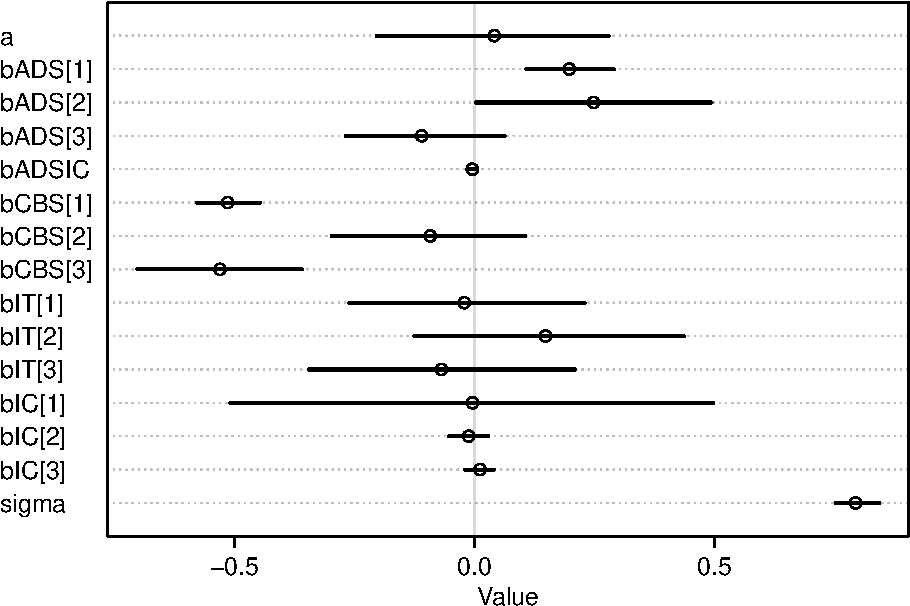
\includegraphics[width=1\linewidth]{bayesianReport3_files/figure-latex/unnamed-chunk-11-1} \end{center}
\normalsize

These, however, are notoriously hard to interpret in models with
interactions. For this reason, it is better to plot predicted effects
for various combinations of predictors.

\vspace{1mm}
\footnotesize

\begin{Shaded}
\begin{Highlighting}[]
\NormalTok{visGroup }\OtherTok{\textless{}{-}} \ControlFlowTok{function}\NormalTok{ (model, ADS, CBS, }\AttributeTok{xmin =}\DecValTok{2}\NormalTok{, }\AttributeTok{ymax =} \SpecialCharTok{{-}}\DecValTok{3}\NormalTok{)}
\NormalTok{\{}
\NormalTok{groupID }\OtherTok{\textless{}{-}} \DecValTok{1}\SpecialCharTok{:}\DecValTok{3}
\NormalTok{IC }\OtherTok{\textless{}{-}} \DecValTok{5} 
\NormalTok{data }\OtherTok{\textless{}{-}} \FunctionTok{expand.grid}\NormalTok{(}\AttributeTok{ADS =}\NormalTok{ ADS,}\AttributeTok{groupID =}\NormalTok{ groupID, }\AttributeTok{CBS =}\NormalTok{ CBS, }\AttributeTok{IC =}\NormalTok{  IC)}
\NormalTok{posterior }\OtherTok{\textless{}{-}} \FunctionTok{extract.samples}\NormalTok{(model, }\AttributeTok{n =} \FloatTok{1e5}\NormalTok{)}
\NormalTok{mu }\OtherTok{\textless{}{-}} \FunctionTok{link}\NormalTok{( model, }\AttributeTok{data=}\NormalTok{data ) }
\FunctionTok{colnames}\NormalTok{(mu) }\OtherTok{\textless{}{-}} \FunctionTok{levels}\NormalTok{(summaries}\SpecialCharTok{$}\NormalTok{group)}
\NormalTok{muLong }\OtherTok{\textless{}{-}} \FunctionTok{melt}\NormalTok{(mu)}
\FunctionTok{colnames}\NormalTok{(muLong) }\OtherTok{\textless{}{-}} \FunctionTok{c}\NormalTok{(}\StringTok{"id"}\NormalTok{, }\StringTok{"group"}\NormalTok{, }\StringTok{"AdiffS"}\NormalTok{)}
\NormalTok{means }\OtherTok{\textless{}{-}}  \FunctionTok{round}\NormalTok{(}\FunctionTok{apply}\NormalTok{(mu , }\DecValTok{2}\NormalTok{ , mean ), }\DecValTok{2}\NormalTok{)}
\NormalTok{mu\_HPDI }\OtherTok{\textless{}{-}} \FunctionTok{round}\NormalTok{(}\FunctionTok{apply}\NormalTok{( mu , }\DecValTok{2}\NormalTok{ , HPDI ),}\DecValTok{2}\NormalTok{)}
\NormalTok{means }\OtherTok{\textless{}{-}} \FunctionTok{as.data.frame}\NormalTok{(means)}
\NormalTok{means}\SpecialCharTok{$}\NormalTok{group }\OtherTok{\textless{}{-}} \FunctionTok{rownames}\NormalTok{(means)}
\FunctionTok{rownames}\NormalTok{(means) }\OtherTok{\textless{}{-}} \ConstantTok{NULL}
\NormalTok{meansDisp }\OtherTok{\textless{}{-}} \FunctionTok{cbind}\NormalTok{(means,}\FunctionTok{t}\NormalTok{(}\FunctionTok{as.data.frame}\NormalTok{(mu\_HPDI)))}
\NormalTok{meansDisp }\OtherTok{\textless{}{-}}\NormalTok{ meansDisp[,}\FunctionTok{c}\NormalTok{(}\DecValTok{1}\NormalTok{,}\DecValTok{3}\NormalTok{,}\DecValTok{4}\NormalTok{)]}

\NormalTok{plot }\OtherTok{\textless{}{-}} \FunctionTok{ggplot}\NormalTok{(muLong)}\SpecialCharTok{+}\FunctionTok{geom\_violin}\NormalTok{(}\FunctionTok{aes}\NormalTok{(}\AttributeTok{x =}\NormalTok{ group, }\AttributeTok{y =}\NormalTok{ AdiffS), }\AttributeTok{alpha =} \FloatTok{0.2}\NormalTok{)}\SpecialCharTok{+}
  \FunctionTok{xlab}\NormalTok{(}\StringTok{""}\NormalTok{)}\SpecialCharTok{+}
  \FunctionTok{labs}\NormalTok{(}\AttributeTok{title =} \FunctionTok{paste}\NormalTok{(}\StringTok{"ADS="}\NormalTok{, ADS, }\StringTok{", CBS="}\NormalTok{,  CBS,  }\AttributeTok{sep =} \StringTok{""}\NormalTok{))}\SpecialCharTok{+}
  \FunctionTok{theme\_tufte}\NormalTok{()}\SpecialCharTok{+}\FunctionTok{ylim}\NormalTok{(}\FunctionTok{c}\NormalTok{(}\SpecialCharTok{{-}}\DecValTok{4}\NormalTok{,}\DecValTok{4}\NormalTok{))}
\CommentTok{\#+   annotation\_custom(tableGrob(meansDisp), xmin=xmin,  ymax=ymax)}
\FunctionTok{return}\NormalTok{(plot)}
\NormalTok{\}}


\NormalTok{visGroupA2C\_2 }\OtherTok{\textless{}{-}} \FunctionTok{visGroup}\NormalTok{(}\AttributeTok{model =}\NormalTok{ FinalHMC, }\AttributeTok{ADS =} \DecValTok{2}\NormalTok{,}\AttributeTok{CBS =} \SpecialCharTok{{-}}\DecValTok{2}\NormalTok{)}
\NormalTok{visGroupA2C0 }\OtherTok{\textless{}{-}} \FunctionTok{visGroup}\NormalTok{(}\AttributeTok{model =}\NormalTok{ FinalHMC, }\AttributeTok{ADS =} \DecValTok{2}\NormalTok{,}\AttributeTok{CBS =} \DecValTok{0}\NormalTok{ )}
\NormalTok{visGroupA2C2 }\OtherTok{\textless{}{-}} \FunctionTok{visGroup}\NormalTok{(}\AttributeTok{model =}\NormalTok{ FinalHMC, }\AttributeTok{ADS =} \DecValTok{2}\NormalTok{,}\AttributeTok{CBS =} \DecValTok{2}\NormalTok{)}

\NormalTok{visGroupA0C\_2 }\OtherTok{\textless{}{-}} \FunctionTok{visGroup}\NormalTok{(}\AttributeTok{model =}\NormalTok{ FinalHMC, }\AttributeTok{ADS =} \DecValTok{0}\NormalTok{,}\AttributeTok{CBS =} \SpecialCharTok{{-}}\DecValTok{2}\NormalTok{ )}
\NormalTok{visGroupA0C0 }\OtherTok{\textless{}{-}} \FunctionTok{visGroup}\NormalTok{(}\AttributeTok{model =}\NormalTok{ FinalHMC, }\AttributeTok{ADS =} \DecValTok{0}\NormalTok{,}\AttributeTok{CBS =} \DecValTok{0}\NormalTok{ )}
\NormalTok{visGroupA0C2 }\OtherTok{\textless{}{-}}  \FunctionTok{visGroup}\NormalTok{(}\AttributeTok{model =}\NormalTok{ FinalHMC, }\AttributeTok{ADS =} \DecValTok{0}\NormalTok{,}\AttributeTok{CBS =} \DecValTok{2}\NormalTok{)}

\NormalTok{visGroupA2C\_2 }\OtherTok{\textless{}{-}}  \FunctionTok{visGroup}\NormalTok{(}\AttributeTok{model =}\NormalTok{ FinalHMC, }\AttributeTok{ADS =} \DecValTok{2}\NormalTok{,}\AttributeTok{CBS =} \SpecialCharTok{{-}}\DecValTok{2}\NormalTok{ )}
\NormalTok{visGroupA2C0 }\OtherTok{\textless{}{-}} \FunctionTok{visGroup}\NormalTok{(}\AttributeTok{model =}\NormalTok{ FinalHMC, }\AttributeTok{ADS =} \DecValTok{2}\NormalTok{,}\AttributeTok{CBS =} \DecValTok{0}\NormalTok{ )}
\NormalTok{visGroupA2C2 }\OtherTok{\textless{}{-}} \FunctionTok{visGroup}\NormalTok{(}\AttributeTok{model =}\NormalTok{ FinalHMC, }\AttributeTok{ADS =} \DecValTok{2}\NormalTok{,}\AttributeTok{CBS =} \DecValTok{2}\NormalTok{ )}

\NormalTok{visGroupJoint }\OtherTok{\textless{}{-}} \FunctionTok{ggarrange}\NormalTok{(visGroupA2C\_2}\SpecialCharTok{+}\NormalTok{removeX }\SpecialCharTok{+} \FunctionTok{ggtitle}\NormalTok{(}\StringTok{"CBS = {-}2"}\NormalTok{)}\SpecialCharTok{+}\FunctionTok{ylab}\NormalTok{(}\StringTok{"ADS = 2"}\NormalTok{) , visGroupA2C0}\SpecialCharTok{+}\FunctionTok{theme\_void}\NormalTok{()}\SpecialCharTok{+} \FunctionTok{ggtitle}\NormalTok{(}\StringTok{"CBS = 0"}\NormalTok{),visGroupA2C2}\SpecialCharTok{+}\FunctionTok{theme\_void}\NormalTok{()}\SpecialCharTok{+} \FunctionTok{ggtitle}\NormalTok{(}\StringTok{"CBS = 2"}\NormalTok{), }
\NormalTok{          visGroupA0C\_2}\SpecialCharTok{+}\NormalTok{removeX}\SpecialCharTok{+}\FunctionTok{ylab}\NormalTok{(}\StringTok{"ADS = 0"}\NormalTok{)}\SpecialCharTok{+}\FunctionTok{ggtitle}\NormalTok{(}\StringTok{""}\NormalTok{), visGroupA0C0}\SpecialCharTok{+}\FunctionTok{theme\_void}\NormalTok{()}\SpecialCharTok{+}\FunctionTok{ggtitle}\NormalTok{(}\StringTok{""}\NormalTok{), visGroupA0C2}\SpecialCharTok{+}\FunctionTok{theme\_void}\NormalTok{()}\SpecialCharTok{+}\FunctionTok{ggtitle}\NormalTok{(}\StringTok{""}\NormalTok{),}
\NormalTok{          visGroupA2C\_2}\SpecialCharTok{+}\FunctionTok{ylab}\NormalTok{(}\StringTok{"ADS = {-}2"}\NormalTok{)}\SpecialCharTok{+}\FunctionTok{ggtitle}\NormalTok{(}\StringTok{""}\NormalTok{), visGroupA2C0}\SpecialCharTok{+}\NormalTok{removeY}\SpecialCharTok{+}\FunctionTok{ggtitle}\NormalTok{(}\StringTok{""}\NormalTok{), visGroupA2C2}\SpecialCharTok{+}\NormalTok{removeY}\SpecialCharTok{+}\FunctionTok{ggtitle}\NormalTok{(}\StringTok{""}\NormalTok{), }\AttributeTok{ncol =}\DecValTok{3}\NormalTok{, }\AttributeTok{nrow =} \DecValTok{3}\NormalTok{)}

 
\NormalTok{visGroupJoint2 }\OtherTok{\textless{}{-}} \FunctionTok{annotate\_figure}\NormalTok{(visGroupJoint, }
  \AttributeTok{top =} \FunctionTok{text\_grob}\NormalTok{(}\StringTok{"(range restricted to ({-}4,4), IC at the rounded mean = 5)"}\NormalTok{,}
                  \AttributeTok{size =} \DecValTok{10}\NormalTok{))}
\NormalTok{visGroupJoint3 }\OtherTok{\textless{}{-}} \FunctionTok{annotate\_figure}\NormalTok{(visGroupJoint2, }
  \AttributeTok{top =} \FunctionTok{text\_grob}\NormalTok{(}\StringTok{"Predicted change in attacks by activity type and treatment groups (standardized)"}\NormalTok{,}
                  \AttributeTok{size =} \DecValTok{12}\NormalTok{))}

\NormalTok{visGroupJoint3 }
\end{Highlighting}
\end{Shaded}

\begin{center}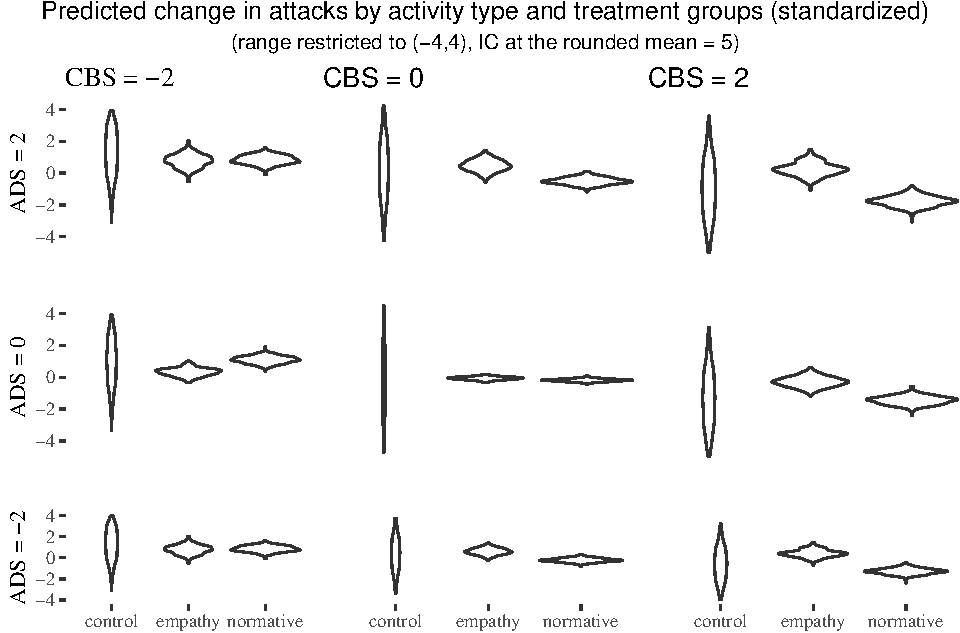
\includegraphics[width=1\linewidth]{bayesianReport3_files/figure-latex/unnamed-chunk-12-1} \end{center}
\normalsize

To gain more clarity, let's look at predicted contrasts, here understood
as distances from the control group mean, by activity types, first
versus CBS, then versus ADS.

\vspace{1mm}
\footnotesize

\begin{Shaded}
\begin{Highlighting}[]
\NormalTok{visContrastsCBS }\OtherTok{\textless{}{-}} \ControlFlowTok{function}\NormalTok{(}\AttributeTok{model =}\NormalTok{ FinalHMC, }\AttributeTok{ADS =}\NormalTok{ ADS , }\AttributeTok{IC =}  \DecValTok{5}\NormalTok{,}
                            \AttributeTok{CBS =} \FunctionTok{seq}\NormalTok{(}\SpecialCharTok{{-}}\DecValTok{3}\NormalTok{,}\DecValTok{3}\NormalTok{,}\AttributeTok{by  =} \FloatTok{0.1}\NormalTok{))}
\NormalTok{  \{}
\NormalTok{  groupID }\OtherTok{\textless{}{-}} \DecValTok{1}\SpecialCharTok{:}\DecValTok{3}
\NormalTok{  data }\OtherTok{\textless{}{-}} \FunctionTok{expand.grid}\NormalTok{(ADS, groupID, IC , CBS)}
  \FunctionTok{colnames}\NormalTok{(data) }\OtherTok{\textless{}{-}} \FunctionTok{c}\NormalTok{(}\StringTok{"ADS"}\NormalTok{, }\StringTok{"groupID"}\NormalTok{, }\StringTok{"IC"}\NormalTok{, }\StringTok{"CBS"}\NormalTok{)}
\NormalTok{  posterior }\OtherTok{\textless{}{-}} \FunctionTok{extract.samples}\NormalTok{(model, }\AttributeTok{n =} \FloatTok{1e5}\NormalTok{)}
  \FunctionTok{link}\NormalTok{( model, }\AttributeTok{data=}\NormalTok{data ) }
\NormalTok{  mu }\OtherTok{\textless{}{-}} \FunctionTok{link}\NormalTok{( model, }\AttributeTok{data=}\NormalTok{data ) }
\NormalTok{  means }\OtherTok{\textless{}{-}}  \FunctionTok{round}\NormalTok{(}\FunctionTok{apply}\NormalTok{(mu , }\DecValTok{2}\NormalTok{ , mean ), }\DecValTok{4}\NormalTok{)}
\NormalTok{  HPDIs }\OtherTok{\textless{}{-}} \FunctionTok{round}\NormalTok{(}\FunctionTok{apply}\NormalTok{( mu , }\DecValTok{2}\NormalTok{ , HPDI ),}\DecValTok{4}\NormalTok{)}
\NormalTok{  visContrast }\OtherTok{\textless{}{-}} \FunctionTok{cbind}\NormalTok{(data,means,}\FunctionTok{t}\NormalTok{(}\FunctionTok{as.data.frame}\NormalTok{(HPDIs)))}
  
\NormalTok{  ones }\OtherTok{\textless{}{-}} \DecValTok{3} \SpecialCharTok{*}\NormalTok{ (}\DecValTok{1}\SpecialCharTok{:}\NormalTok{(}\FunctionTok{nrow}\NormalTok{(visContrast)}\SpecialCharTok{/}\DecValTok{3}\NormalTok{))}\SpecialCharTok{{-}}\DecValTok{2}
\NormalTok{  twos }\OtherTok{\textless{}{-}} \DecValTok{3} \SpecialCharTok{*}\NormalTok{ (}\DecValTok{1}\SpecialCharTok{:}\NormalTok{(}\FunctionTok{nrow}\NormalTok{(visContrast)}\SpecialCharTok{/}\DecValTok{3}\NormalTok{))}\SpecialCharTok{{-}}\DecValTok{1}
\NormalTok{  threes }\OtherTok{\textless{}{-}} \DecValTok{3} \SpecialCharTok{*}\NormalTok{ (}\DecValTok{1}\SpecialCharTok{:}\NormalTok{(}\FunctionTok{nrow}\NormalTok{(visContrast)}\SpecialCharTok{/}\DecValTok{3}\NormalTok{))}
  
  \FunctionTok{colnames}\NormalTok{(visContrast)[}\FunctionTok{c}\NormalTok{(}\DecValTok{6}\NormalTok{,}\DecValTok{7}\NormalTok{)] }\OtherTok{\textless{}{-}} \FunctionTok{c}\NormalTok{(}\StringTok{"low"}\NormalTok{, }\StringTok{"high"}\NormalTok{)}
\NormalTok{  contrast }\OtherTok{\textless{}{-}} \FunctionTok{numeric}\NormalTok{(}\FunctionTok{nrow}\NormalTok{(visContrast))}
\NormalTok{  cLow }\OtherTok{\textless{}{-}} \FunctionTok{numeric}\NormalTok{(}\FunctionTok{nrow}\NormalTok{(visContrast))}
\NormalTok{  cHigh }\OtherTok{\textless{}{-}} \FunctionTok{numeric}\NormalTok{(}\FunctionTok{nrow}\NormalTok{(visContrast))}
  \ControlFlowTok{for}\NormalTok{(i }\ControlFlowTok{in}\NormalTok{ threes)\{}
\NormalTok{  contrast[i] }\OtherTok{\textless{}{-}}\NormalTok{ visContrast}\SpecialCharTok{$}\NormalTok{means[i] }\SpecialCharTok{{-}}\NormalTok{ visContrast}\SpecialCharTok{$}\NormalTok{means[i}\DecValTok{{-}2}\NormalTok{]  }
\NormalTok{  \}}
  \ControlFlowTok{for}\NormalTok{(i }\ControlFlowTok{in}\NormalTok{ twos)\{}
\NormalTok{  contrast[i] }\OtherTok{\textless{}{-}}\NormalTok{ visContrast}\SpecialCharTok{$}\NormalTok{means[i] }\SpecialCharTok{{-}}\NormalTok{ visContrast}\SpecialCharTok{$}\NormalTok{means[i}\DecValTok{{-}1}\NormalTok{]  }
\NormalTok{  \}}
\NormalTok{  visContrast}\SpecialCharTok{$}\NormalTok{contrast }\OtherTok{\textless{}{-}}\NormalTok{ contrast}
\NormalTok{  visContrast}\SpecialCharTok{$}\NormalTok{shift }\OtherTok{\textless{}{-}}\NormalTok{  visContrast}\SpecialCharTok{$}\NormalTok{contrast }\SpecialCharTok{{-}}\NormalTok{ visContrast}\SpecialCharTok{$}\NormalTok{means}
  \ControlFlowTok{for}\NormalTok{(i }\ControlFlowTok{in}\NormalTok{ ones)\{}
\NormalTok{  visContrast}\SpecialCharTok{$}\NormalTok{shift[i] }\OtherTok{\textless{}{-}} \DecValTok{0}
\NormalTok{  \}}
\NormalTok{  visContrast}\SpecialCharTok{$}\NormalTok{cLow }\OtherTok{\textless{}{-}}\NormalTok{ visContrast}\SpecialCharTok{$}\NormalTok{low }\SpecialCharTok{+}\NormalTok{ visContrast}\SpecialCharTok{$}\NormalTok{shift}
\NormalTok{  visContrast}\SpecialCharTok{$}\NormalTok{cHigh }\OtherTok{\textless{}{-}}\NormalTok{ visContrast}\SpecialCharTok{$}\NormalTok{high }\SpecialCharTok{+}\NormalTok{ visContrast}\SpecialCharTok{$}\NormalTok{shift}

\NormalTok{  visContrast}\SpecialCharTok{$}\NormalTok{group }\OtherTok{=} \FunctionTok{rep}\NormalTok{(}\FunctionTok{c}\NormalTok{(}\StringTok{"control"}\NormalTok{, }\StringTok{"empathy"}\NormalTok{, }\StringTok{"normative"}\NormalTok{), }
                          \FunctionTok{nrow}\NormalTok{(visContrast)}\SpecialCharTok{/}\DecValTok{3}\NormalTok{)}

\NormalTok{  visContrastTreatment }\OtherTok{\textless{}{-}}\NormalTok{ visContrast[groupID }\SpecialCharTok{!=}\DecValTok{1}\NormalTok{,]}

  \FunctionTok{return}\NormalTok{(}\FunctionTok{ggplot}\NormalTok{(visContrastTreatment, }\FunctionTok{aes}\NormalTok{(}\AttributeTok{x =}\NormalTok{ CBS, }\AttributeTok{y =}\NormalTok{ contrast, }\AttributeTok{fill =}\NormalTok{ group ))}\SpecialCharTok{+}
           \FunctionTok{geom\_line}\NormalTok{(}\AttributeTok{se =} \ConstantTok{FALSE}\NormalTok{)}\SpecialCharTok{+}
            \FunctionTok{geom\_ribbon}\NormalTok{(}\AttributeTok{mapping =} 
        \FunctionTok{aes}\NormalTok{(}\AttributeTok{ymin =}\NormalTok{ cLow, }\AttributeTok{ymax =}\NormalTok{ cHigh),  }
         \AttributeTok{alpha =}\NormalTok{ .}\DecValTok{3}\NormalTok{)}\SpecialCharTok{+}
          \FunctionTok{theme\_tufte}\NormalTok{())}
\NormalTok{\}}


\NormalTok{visContrastCBSJoint }\OtherTok{\textless{}{-}} \FunctionTok{ggarrange}\NormalTok{(}\FunctionTok{visContrastsCBS}\NormalTok{(FinalHMC,}\AttributeTok{ADS =} \SpecialCharTok{{-}}\DecValTok{2}\NormalTok{)}\SpecialCharTok{+}
      \FunctionTok{ggtitle}\NormalTok{(}\StringTok{"ADS = {-}2"}\NormalTok{)}\SpecialCharTok{+}\FunctionTok{ylim}\NormalTok{(}\FunctionTok{c}\NormalTok{(}\SpecialCharTok{{-}}\FloatTok{2.5}\NormalTok{,}\FloatTok{2.5}\NormalTok{))}\SpecialCharTok{+} \FunctionTok{scale\_fill\_discrete}\NormalTok{(}\AttributeTok{guide=}\ConstantTok{FALSE}\NormalTok{),}
          \FunctionTok{visContrastsCBS}\NormalTok{(FinalHMC,}\AttributeTok{ADS =} \DecValTok{0}\NormalTok{)}\SpecialCharTok{+}\FunctionTok{ggtitle}\NormalTok{(}\StringTok{"ADS = 0"}\NormalTok{)}\SpecialCharTok{+}
        \FunctionTok{ylim}\NormalTok{(}\FunctionTok{c}\NormalTok{(}\SpecialCharTok{{-}}\FloatTok{2.5}\NormalTok{,}\FloatTok{2.5}\NormalTok{))}\SpecialCharTok{+} \FunctionTok{scale\_fill\_discrete}\NormalTok{(}\AttributeTok{guide=}\ConstantTok{FALSE}\NormalTok{)}\SpecialCharTok{+}
\NormalTok{        removeY,}
        \FunctionTok{visContrastsCBS}\NormalTok{(FinalHMC,}\AttributeTok{ADS =} \DecValTok{2}\NormalTok{)}\SpecialCharTok{+}\FunctionTok{ggtitle}\NormalTok{(}\StringTok{"ADS = 2"}\NormalTok{)}\SpecialCharTok{+}
        \FunctionTok{ylim}\NormalTok{(}\FunctionTok{c}\NormalTok{(}\SpecialCharTok{{-}}\FloatTok{2.5}\NormalTok{,}\FloatTok{2.5}\NormalTok{))}\SpecialCharTok{+} \FunctionTok{theme}\NormalTok{(}\AttributeTok{legend.position =} \FunctionTok{c}\NormalTok{(}\FloatTok{0.75}\NormalTok{, }\FloatTok{0.15}\NormalTok{))}\SpecialCharTok{+}
\NormalTok{        removeY, }\AttributeTok{ncol =} \DecValTok{3}\NormalTok{)}

\NormalTok{visContrastCBSJoint2 }\OtherTok{\textless{}{-}} \FunctionTok{annotate\_figure}\NormalTok{(visContrastCBSJoint, }
      \AttributeTok{top =} \FunctionTok{text\_grob}\NormalTok{(}\StringTok{"(range restricted to ({-}2.5,2.5), IC at the rounded mean = 5)"}\NormalTok{,}
                                \AttributeTok{size =} \DecValTok{10}\NormalTok{))}
\NormalTok{visContrastCBSJoint3 }\OtherTok{\textless{}{-}} \FunctionTok{annotate\_figure}\NormalTok{(visContrastCBSJoint2, }
\AttributeTok{top =} \FunctionTok{text\_grob}\NormalTok{(}\StringTok{"Predicted distance from the control group mean vs. CBS  (standardized)"}\NormalTok{,}
                                \AttributeTok{size =} \DecValTok{12}\NormalTok{))}

\NormalTok{visContrastCBSJoint3}
\end{Highlighting}
\end{Shaded}

\begin{center}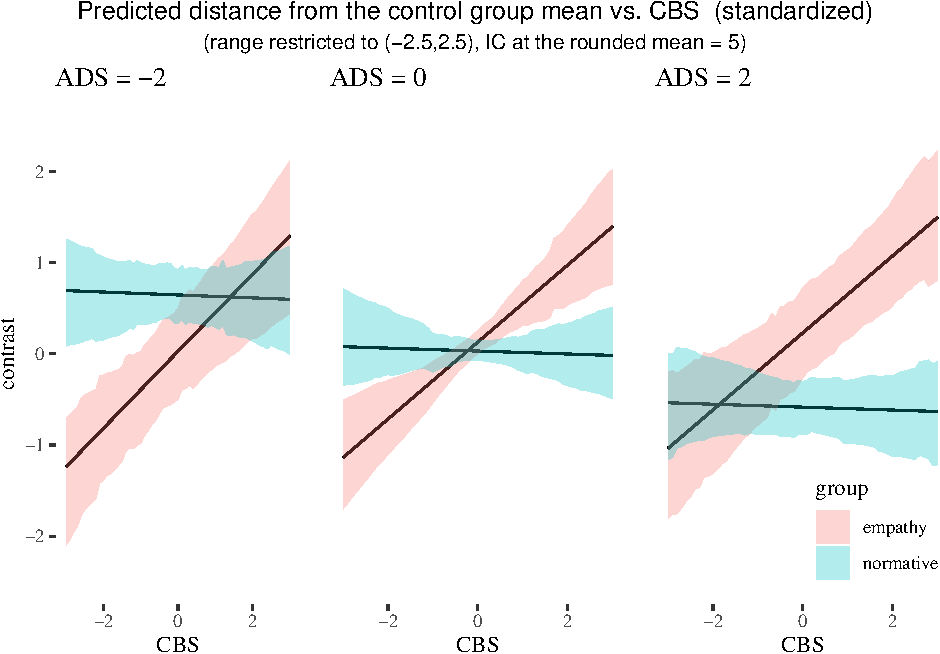
\includegraphics[width=1\linewidth]{bayesianReport3_files/figure-latex/unnamed-chunk-13-1} \end{center}
\normalsize

\vspace{1mm}
\footnotesize

\begin{Shaded}
\begin{Highlighting}[]
\NormalTok{visContrastsADS }\OtherTok{\textless{}{-}} \ControlFlowTok{function}\NormalTok{(}\AttributeTok{model =}\NormalTok{ FinalHMC, }\AttributeTok{CBS =}\NormalTok{ CBS , }\AttributeTok{IC =}  \DecValTok{5}\NormalTok{, }
                            \AttributeTok{ADS =} \FunctionTok{seq}\NormalTok{(}\SpecialCharTok{{-}}\DecValTok{3}\NormalTok{,}\DecValTok{3}\NormalTok{,}\AttributeTok{by  =} \FloatTok{0.1}\NormalTok{))}
\NormalTok{\{}
\NormalTok{  data }\OtherTok{\textless{}{-}} \FunctionTok{expand.grid}\NormalTok{(CBS, groupID, IC , ADS)}
  \FunctionTok{colnames}\NormalTok{(data) }\OtherTok{\textless{}{-}} \FunctionTok{c}\NormalTok{(}\StringTok{"CBS"}\NormalTok{, }\StringTok{"groupID"}\NormalTok{, }\StringTok{"IC"}\NormalTok{, }\StringTok{"ADS"}\NormalTok{)}
\NormalTok{  posterior }\OtherTok{\textless{}{-}} \FunctionTok{extract.samples}\NormalTok{(model, }\AttributeTok{n =} \FloatTok{1e5}\NormalTok{)}
\NormalTok{  mu }\OtherTok{\textless{}{-}} \FunctionTok{link}\NormalTok{( model, }\AttributeTok{data=}\NormalTok{data ) }
\NormalTok{  means }\OtherTok{\textless{}{-}}  \FunctionTok{round}\NormalTok{(}\FunctionTok{apply}\NormalTok{(mu , }\DecValTok{2}\NormalTok{ , mean ), }\DecValTok{4}\NormalTok{)}
\NormalTok{  HPDIs }\OtherTok{\textless{}{-}} \FunctionTok{round}\NormalTok{(}\FunctionTok{apply}\NormalTok{( mu , }\DecValTok{2}\NormalTok{ , HPDI ),}\DecValTok{4}\NormalTok{)}
\NormalTok{  visContrastADS }\OtherTok{\textless{}{-}} \FunctionTok{cbind}\NormalTok{(data,means,}\FunctionTok{t}\NormalTok{(}\FunctionTok{as.data.frame}\NormalTok{(HPDIs)))}


\NormalTok{  ones }\OtherTok{\textless{}{-}} \DecValTok{3} \SpecialCharTok{*}\NormalTok{ (}\DecValTok{1}\SpecialCharTok{:}\NormalTok{(}\FunctionTok{nrow}\NormalTok{(visContrastADS)}\SpecialCharTok{/}\DecValTok{3}\NormalTok{))}\SpecialCharTok{{-}}\DecValTok{2}
\NormalTok{  twos }\OtherTok{\textless{}{-}} \DecValTok{3} \SpecialCharTok{*}\NormalTok{ (}\DecValTok{1}\SpecialCharTok{:}\NormalTok{(}\FunctionTok{nrow}\NormalTok{(visContrastADS)}\SpecialCharTok{/}\DecValTok{3}\NormalTok{))}\SpecialCharTok{{-}}\DecValTok{1}
\NormalTok{  threes }\OtherTok{\textless{}{-}} \DecValTok{3} \SpecialCharTok{*}\NormalTok{ (}\DecValTok{1}\SpecialCharTok{:}\NormalTok{(}\FunctionTok{nrow}\NormalTok{(visContrastADS)}\SpecialCharTok{/}\DecValTok{3}\NormalTok{))}
  
  \FunctionTok{colnames}\NormalTok{(visContrastADS)[}\FunctionTok{c}\NormalTok{(}\DecValTok{6}\NormalTok{,}\DecValTok{7}\NormalTok{)] }\OtherTok{\textless{}{-}} \FunctionTok{c}\NormalTok{(}\StringTok{"low"}\NormalTok{, }\StringTok{"high"}\NormalTok{)}
\NormalTok{  contrastADS }\OtherTok{\textless{}{-}} \FunctionTok{numeric}\NormalTok{(}\FunctionTok{nrow}\NormalTok{(visContrastADS))}
  \ControlFlowTok{for}\NormalTok{(i }\ControlFlowTok{in}\NormalTok{ threes)\{}
\NormalTok{    contrastADS[i] }\OtherTok{\textless{}{-}}\NormalTok{ visContrastADS}\SpecialCharTok{$}\NormalTok{means[i] }\SpecialCharTok{{-}}\NormalTok{ visContrastADS}\SpecialCharTok{$}\NormalTok{means[i}\DecValTok{{-}2}\NormalTok{]  }
\NormalTok{  \}}
  \ControlFlowTok{for}\NormalTok{(i }\ControlFlowTok{in}\NormalTok{ twos)\{}
\NormalTok{    contrastADS[i] }\OtherTok{\textless{}{-}}\NormalTok{ visContrastADS}\SpecialCharTok{$}\NormalTok{means[i] }\SpecialCharTok{{-}}\NormalTok{ visContrastADS}\SpecialCharTok{$}\NormalTok{means[i}\DecValTok{{-}1}\NormalTok{]  }
\NormalTok{  \}}
\NormalTok{  visContrastADS}\SpecialCharTok{$}\NormalTok{contrast }\OtherTok{\textless{}{-}}\NormalTok{ contrastADS}
\NormalTok{  visContrastADS}\SpecialCharTok{$}\NormalTok{shift }\OtherTok{\textless{}{-}}\NormalTok{  visContrastADS}\SpecialCharTok{$}\NormalTok{contrast }\SpecialCharTok{{-}}\NormalTok{ visContrastADS}\SpecialCharTok{$}\NormalTok{means}
  \ControlFlowTok{for}\NormalTok{(i }\ControlFlowTok{in}\NormalTok{ ones)\{}
\NormalTok{    visContrastADS}\SpecialCharTok{$}\NormalTok{shift[i] }\OtherTok{\textless{}{-}} \DecValTok{0}
\NormalTok{  \}}
\NormalTok{  visContrastADS}\SpecialCharTok{$}\NormalTok{cLow }\OtherTok{\textless{}{-}}\NormalTok{ visContrastADS}\SpecialCharTok{$}\NormalTok{low }\SpecialCharTok{+}\NormalTok{ visContrastADS}\SpecialCharTok{$}\NormalTok{shift}
\NormalTok{  visContrastADS}\SpecialCharTok{$}\NormalTok{cHigh }\OtherTok{\textless{}{-}}\NormalTok{ visContrastADS}\SpecialCharTok{$}\NormalTok{high }\SpecialCharTok{+}\NormalTok{ visContrastADS}\SpecialCharTok{$}\NormalTok{shift}
  
\NormalTok{  visContrastADS}\SpecialCharTok{$}\NormalTok{group }\OtherTok{=} \FunctionTok{rep}\NormalTok{(}\FunctionTok{c}\NormalTok{(}\StringTok{"control"}\NormalTok{, }\StringTok{"empathy"}\NormalTok{, }\StringTok{"normative"}\NormalTok{), }
                             \FunctionTok{nrow}\NormalTok{(visContrastADS)}\SpecialCharTok{/}\DecValTok{3}\NormalTok{)}
\NormalTok{  visContrastTreatmentADS }\OtherTok{\textless{}{-}}\NormalTok{ visContrastADS[groupID }\SpecialCharTok{!=}\DecValTok{1}\NormalTok{,]}

  \FunctionTok{return}\NormalTok{(}\FunctionTok{ggplot}\NormalTok{(visContrastTreatmentADS, }\FunctionTok{aes}\NormalTok{(}\AttributeTok{x =}\NormalTok{ ADS, }\AttributeTok{y =}\NormalTok{ contrast, }\AttributeTok{fill =}\NormalTok{ group ))}\SpecialCharTok{+}
           \FunctionTok{geom\_line}\NormalTok{(}\AttributeTok{se =} \ConstantTok{FALSE}\NormalTok{) }\SpecialCharTok{+}
  \FunctionTok{geom\_ribbon}\NormalTok{(}\AttributeTok{mapping =} \FunctionTok{aes}\NormalTok{(}\AttributeTok{ymin =}\NormalTok{ cLow, }\AttributeTok{ymax =}\NormalTok{ cHigh), }
       \AttributeTok{alpha =}\NormalTok{ .}\DecValTok{3}\NormalTok{) }\SpecialCharTok{+}\FunctionTok{theme\_tufte}\NormalTok{())}
\NormalTok{\}}



\NormalTok{visContrastADSJoint }\OtherTok{\textless{}{-}} \FunctionTok{ggarrange}\NormalTok{(}\FunctionTok{visContrastsADS}\NormalTok{(FinalHMC,}\AttributeTok{CBS =} \SpecialCharTok{{-}}\DecValTok{2}\NormalTok{)}\SpecialCharTok{+}\FunctionTok{ggtitle}\NormalTok{(}\StringTok{"CBS = {-}2"}\NormalTok{)}
                                 \SpecialCharTok{+}\FunctionTok{ylim}\NormalTok{(}\FunctionTok{c}\NormalTok{(}\SpecialCharTok{{-}}\FloatTok{2.5}\NormalTok{,}\FloatTok{2.5}\NormalTok{))}\SpecialCharTok{+} \FunctionTok{scale\_fill\_discrete}\NormalTok{(}\AttributeTok{guide=}\ConstantTok{FALSE}\NormalTok{),}
                                 \FunctionTok{visContrastsADS}\NormalTok{(FinalHMC,}\AttributeTok{CBS =} \DecValTok{0}\NormalTok{)}\SpecialCharTok{+}\FunctionTok{ggtitle}\NormalTok{(}\StringTok{"CBS = 0"}\NormalTok{)}
                                 \SpecialCharTok{+}\FunctionTok{ylim}\NormalTok{(}\FunctionTok{c}\NormalTok{(}\SpecialCharTok{{-}}\FloatTok{2.5}\NormalTok{,}\FloatTok{2.5}\NormalTok{))}\SpecialCharTok{+} \FunctionTok{scale\_fill\_discrete}\NormalTok{(}\AttributeTok{guide=}\ConstantTok{FALSE}\NormalTok{)}\SpecialCharTok{+}
\NormalTok{                                   removeY,}
                                 \FunctionTok{visContrastsADS}\NormalTok{(FinalHMC,}\AttributeTok{CBS =} \DecValTok{2}\NormalTok{)}\SpecialCharTok{+}\FunctionTok{ggtitle}\NormalTok{(}\StringTok{"CBS = 2"}\NormalTok{)}
                                 \SpecialCharTok{+}\FunctionTok{ylim}\NormalTok{(}\FunctionTok{c}\NormalTok{(}\SpecialCharTok{{-}}\FloatTok{2.5}\NormalTok{,}\FloatTok{2.5}\NormalTok{))}\SpecialCharTok{+}
                                   \FunctionTok{theme}\NormalTok{(}\AttributeTok{legend.position =} \FunctionTok{c}\NormalTok{(}\FloatTok{0.75}\NormalTok{, }\FloatTok{0.15}\NormalTok{))}\SpecialCharTok{+}
\NormalTok{                                   removeY, }\AttributeTok{ncol =} \DecValTok{3}\NormalTok{)}

\NormalTok{visContrastADSJoint2 }\OtherTok{\textless{}{-}} \FunctionTok{annotate\_figure}\NormalTok{(visContrastADSJoint, }
\AttributeTok{top =} \FunctionTok{text\_grob}\NormalTok{(}\StringTok{"(range restricted to ({-}2.5,2.5), IC at the rounded mean = 5)"}\NormalTok{,}
                                                        \AttributeTok{size =} \DecValTok{10}\NormalTok{))}
\NormalTok{visContrastADSJoint3 }\OtherTok{\textless{}{-}} \FunctionTok{annotate\_figure}\NormalTok{(visContrastADSJoint2, }
\AttributeTok{top =} \FunctionTok{text\_grob}\NormalTok{(}\StringTok{"Predicted distance from the control group mean vs. ADS (standardized)"}\NormalTok{,}
                                                        \AttributeTok{size =} \DecValTok{12}\NormalTok{))}

\NormalTok{visContrastADSJoint3}
\end{Highlighting}
\end{Shaded}

\begin{center}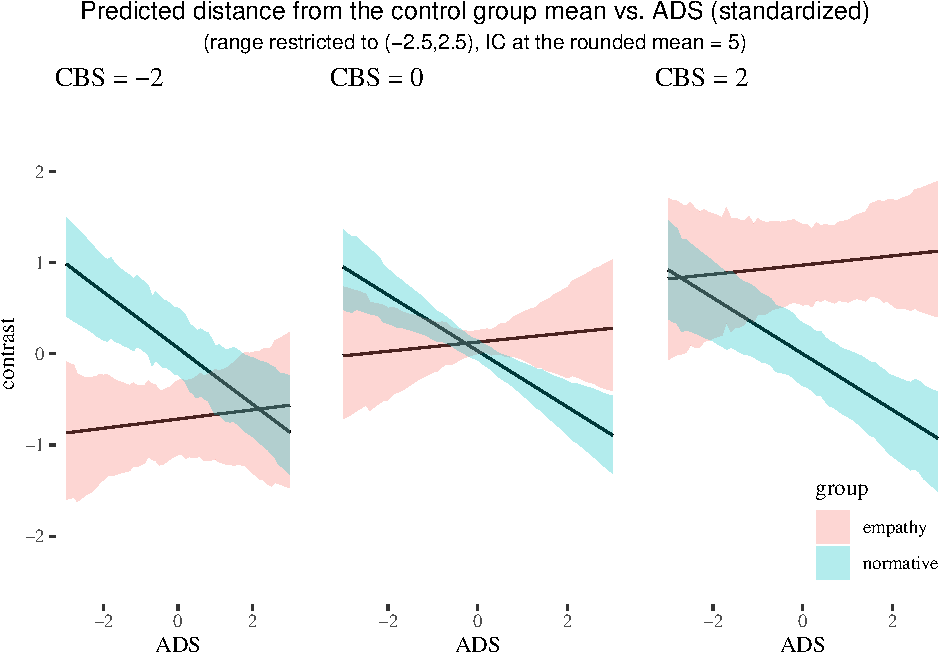
\includegraphics[width=1\linewidth]{bayesianReport3_files/figure-latex/unnamed-chunk-14-1} \end{center}
\normalsize

Now, let's inspect the impact of intervention counts by treatment type
by looking at contrasts (distances from the control group mean) with
89\% HPDIs by IC. Notice the predicted effect of \textsf{IC} is weaker
than group membership, so for visibility the \(y\)-axis has a smaller
range. Also, not enough data was available to reliably estimate
uncertainty for \textsf{IC} above 20, hence the restriction on the
\(x\)-axis (arleady at lower values, lack of estimates is visible for
the more extreme covariate settings).

\vspace{1mm}
\footnotesize

\begin{Shaded}
\begin{Highlighting}[]
\NormalTok{visContrastsIC }\OtherTok{\textless{}{-}} \ControlFlowTok{function}\NormalTok{(}\AttributeTok{model =}\NormalTok{ FinalHMC, }\AttributeTok{CBS =}\NormalTok{ CBS ,}
                           \AttributeTok{IC =}  \FunctionTok{seq}\NormalTok{(}\DecValTok{0}\NormalTok{,}\DecValTok{20}\NormalTok{,}\AttributeTok{by =} \DecValTok{1}\NormalTok{), }\AttributeTok{ADS =}\NormalTok{ ADS)}
\NormalTok{\{}
\NormalTok{  groupID }\OtherTok{\textless{}{-}} \DecValTok{1}\SpecialCharTok{:}\DecValTok{3}
\NormalTok{  data }\OtherTok{\textless{}{-}} \FunctionTok{expand.grid}\NormalTok{(CBS, groupID, IC , ADS)}
\NormalTok{  data}
  \FunctionTok{colnames}\NormalTok{(data) }\OtherTok{\textless{}{-}} \FunctionTok{c}\NormalTok{(}\StringTok{"CBS"}\NormalTok{, }\StringTok{"groupID"}\NormalTok{, }\StringTok{"IC"}\NormalTok{, }\StringTok{"ADS"}\NormalTok{)}
\NormalTok{  posterior }\OtherTok{\textless{}{-}} \FunctionTok{extract.samples}\NormalTok{(model, }\AttributeTok{n =} \FloatTok{1e5}\NormalTok{)}
\NormalTok{  mu }\OtherTok{\textless{}{-}} \FunctionTok{link}\NormalTok{( model, }\AttributeTok{data=}\NormalTok{data ) }
\NormalTok{  means }\OtherTok{\textless{}{-}}  \FunctionTok{round}\NormalTok{(}\FunctionTok{apply}\NormalTok{(mu , }\DecValTok{2}\NormalTok{ , mean ), }\DecValTok{4}\NormalTok{)}
\NormalTok{  HPDIs }\OtherTok{\textless{}{-}} \FunctionTok{round}\NormalTok{(}\FunctionTok{apply}\NormalTok{( mu , }\DecValTok{2}\NormalTok{ , HPDI ),}\DecValTok{4}\NormalTok{)}
\NormalTok{  visContrastIC }\OtherTok{\textless{}{-}} \FunctionTok{cbind}\NormalTok{(data,means,}\FunctionTok{t}\NormalTok{(}\FunctionTok{as.data.frame}\NormalTok{(HPDIs)))}
  
\NormalTok{  ones }\OtherTok{\textless{}{-}} \DecValTok{3} \SpecialCharTok{*}\NormalTok{ (}\DecValTok{1}\SpecialCharTok{:}\NormalTok{(}\FunctionTok{nrow}\NormalTok{(visContrastIC)}\SpecialCharTok{/}\DecValTok{3}\NormalTok{))}\SpecialCharTok{{-}}\DecValTok{2}
\NormalTok{  twos }\OtherTok{\textless{}{-}} \DecValTok{3} \SpecialCharTok{*}\NormalTok{ (}\DecValTok{1}\SpecialCharTok{:}\NormalTok{(}\FunctionTok{nrow}\NormalTok{(visContrastIC)}\SpecialCharTok{/}\DecValTok{3}\NormalTok{))}\SpecialCharTok{{-}}\DecValTok{1}
\NormalTok{  threes }\OtherTok{\textless{}{-}} \DecValTok{3} \SpecialCharTok{*}\NormalTok{ (}\DecValTok{1}\SpecialCharTok{:}\NormalTok{(}\FunctionTok{nrow}\NormalTok{(visContrastIC)}\SpecialCharTok{/}\DecValTok{3}\NormalTok{))}
  
  \FunctionTok{colnames}\NormalTok{(visContrastIC)[}\FunctionTok{c}\NormalTok{(}\DecValTok{6}\NormalTok{,}\DecValTok{7}\NormalTok{)] }\OtherTok{\textless{}{-}} \FunctionTok{c}\NormalTok{(}\StringTok{"low"}\NormalTok{, }\StringTok{"high"}\NormalTok{)}
\NormalTok{  contrastIC }\OtherTok{\textless{}{-}} \FunctionTok{numeric}\NormalTok{(}\FunctionTok{nrow}\NormalTok{(visContrastIC))}
  \ControlFlowTok{for}\NormalTok{(i }\ControlFlowTok{in}\NormalTok{ threes)\{}
\NormalTok{    contrastIC[i] }\OtherTok{\textless{}{-}}\NormalTok{ visContrastIC}\SpecialCharTok{$}\NormalTok{means[i] }\SpecialCharTok{{-}}\NormalTok{ visContrastIC}\SpecialCharTok{$}\NormalTok{means[i}\DecValTok{{-}2}\NormalTok{]  }
\NormalTok{  \}}
  \ControlFlowTok{for}\NormalTok{(i }\ControlFlowTok{in}\NormalTok{ twos)\{}
\NormalTok{    contrastIC[i] }\OtherTok{\textless{}{-}}\NormalTok{ visContrastIC}\SpecialCharTok{$}\NormalTok{means[i] }\SpecialCharTok{{-}}\NormalTok{ visContrastIC}\SpecialCharTok{$}\NormalTok{means[i}\DecValTok{{-}1}\NormalTok{]  }
\NormalTok{  \}}
\NormalTok{  visContrastIC}\SpecialCharTok{$}\NormalTok{contrast }\OtherTok{\textless{}{-}}\NormalTok{ contrastIC}
\NormalTok{  visContrastIC}\SpecialCharTok{$}\NormalTok{shift }\OtherTok{\textless{}{-}}\NormalTok{  visContrastIC}\SpecialCharTok{$}\NormalTok{contrast }\SpecialCharTok{{-}}\NormalTok{ visContrastIC}\SpecialCharTok{$}\NormalTok{means}
  \ControlFlowTok{for}\NormalTok{(i }\ControlFlowTok{in}\NormalTok{ ones)\{}
\NormalTok{    visContrastIC}\SpecialCharTok{$}\NormalTok{shift[i] }\OtherTok{\textless{}{-}} \DecValTok{0}
\NormalTok{  \}}
\NormalTok{  visContrastIC}\SpecialCharTok{$}\NormalTok{cLow }\OtherTok{\textless{}{-}}\NormalTok{ visContrastIC}\SpecialCharTok{$}\NormalTok{low }\SpecialCharTok{+}\NormalTok{ visContrastIC}\SpecialCharTok{$}\NormalTok{shift}
\NormalTok{  visContrastIC}\SpecialCharTok{$}\NormalTok{cHigh }\OtherTok{\textless{}{-}}\NormalTok{ visContrastIC}\SpecialCharTok{$}\NormalTok{high }\SpecialCharTok{+}\NormalTok{ visContrastIC}\SpecialCharTok{$}\NormalTok{shift}
  
\NormalTok{  visContrastIC}\SpecialCharTok{$}\NormalTok{group }\OtherTok{=} \FunctionTok{rep}\NormalTok{(}\FunctionTok{c}\NormalTok{(}\StringTok{"control"}\NormalTok{, }\StringTok{"empathy"}\NormalTok{, }\StringTok{"normative"}\NormalTok{),}
                            \FunctionTok{nrow}\NormalTok{(visContrastIC)}\SpecialCharTok{/}\DecValTok{3}\NormalTok{)}
\NormalTok{  visContrastTreatmentIC }\OtherTok{\textless{}{-}}\NormalTok{ visContrastIC[groupID }\SpecialCharTok{!=}\DecValTok{1}\NormalTok{,]}
  
  \FunctionTok{return}\NormalTok{(}\FunctionTok{ggplot}\NormalTok{(visContrastTreatmentIC, }\FunctionTok{aes}\NormalTok{(}\AttributeTok{x =}\NormalTok{ IC, }\AttributeTok{y =}\NormalTok{ contrast, }\AttributeTok{fill =}\NormalTok{ group ))}\SpecialCharTok{+}
           \FunctionTok{geom\_line}\NormalTok{(}\AttributeTok{se=}\ConstantTok{FALSE}\NormalTok{)}\SpecialCharTok{+}
    \FunctionTok{geom\_ribbon}\NormalTok{(}\AttributeTok{mapping =} \FunctionTok{aes}\NormalTok{(}\AttributeTok{ymin =}\NormalTok{ cLow, }\AttributeTok{ymax =}\NormalTok{ cHigh), }\AttributeTok{alpha =}\NormalTok{ .}\DecValTok{3}\NormalTok{)}\SpecialCharTok{+}
    \FunctionTok{ylim}\NormalTok{(}\FunctionTok{c}\NormalTok{(}\SpecialCharTok{{-}}\DecValTok{2}\NormalTok{,}\DecValTok{2}\NormalTok{)) }\SpecialCharTok{+}\FunctionTok{theme\_tufte}\NormalTok{()}\SpecialCharTok{+}\FunctionTok{geom\_hline}\NormalTok{(}\AttributeTok{yintercept =} \DecValTok{0}\NormalTok{, }\AttributeTok{lty =}\DecValTok{2}\NormalTok{, }\AttributeTok{size =} \FloatTok{0.1}\NormalTok{))}
\NormalTok{\}}


\NormalTok{visContrastsICJoint }\OtherTok{\textless{}{-}} \FunctionTok{ggarrange}\NormalTok{(}
\FunctionTok{visContrastsIC}\NormalTok{(}\AttributeTok{ADS =} \DecValTok{2}\NormalTok{, }\AttributeTok{CBS =} \SpecialCharTok{{-}}\DecValTok{2}\NormalTok{)}\SpecialCharTok{+}\NormalTok{removeX}\SpecialCharTok{+} 
               \FunctionTok{theme}\NormalTok{(}\AttributeTok{legend.position =} \FunctionTok{c}\NormalTok{(}\FloatTok{0.3}\NormalTok{, }\FloatTok{0.9}\NormalTok{),}
                     \AttributeTok{legend.key.size =} \FunctionTok{unit}\NormalTok{(.}\DecValTok{3}\NormalTok{, }\StringTok{\textquotesingle{}cm\textquotesingle{}}\NormalTok{),}
                     \AttributeTok{legend.key.height =} \FunctionTok{unit}\NormalTok{(.}\DecValTok{3}\NormalTok{, }\StringTok{\textquotesingle{}cm\textquotesingle{}}\NormalTok{),}
                     \AttributeTok{legend.key.width =} \FunctionTok{unit}\NormalTok{(.}\DecValTok{3}\NormalTok{, }\StringTok{\textquotesingle{}cm\textquotesingle{}}\NormalTok{),}
                     \AttributeTok{legend.title=} \FunctionTok{element\_blank}\NormalTok{())}\SpecialCharTok{+}
  \FunctionTok{ggtitle}\NormalTok{(}\StringTok{"CBS = {-}2"}\NormalTok{)}\SpecialCharTok{+}
  \FunctionTok{ylab}\NormalTok{(}\StringTok{"ADS = 2"}\NormalTok{),}
    \FunctionTok{visContrastsIC}\NormalTok{(}\AttributeTok{ADS =} \DecValTok{2}\NormalTok{, }\AttributeTok{CBS =} \DecValTok{0}\NormalTok{)}\SpecialCharTok{+}\NormalTok{removeY}\SpecialCharTok{+}\NormalTok{removeX}\SpecialCharTok{+} \FunctionTok{scale\_fill\_discrete}\NormalTok{(}\AttributeTok{guide=}\ConstantTok{FALSE}\NormalTok{)}\SpecialCharTok{+}
  \FunctionTok{ggtitle}\NormalTok{(}\StringTok{"CBS = 0"}\NormalTok{),}
    \FunctionTok{visContrastsIC}\NormalTok{(}\AttributeTok{ADS =} \DecValTok{2}\NormalTok{, }\AttributeTok{CBS =} \DecValTok{2}\NormalTok{)}\SpecialCharTok{+}\NormalTok{removeY}\SpecialCharTok{+}\NormalTok{removeX}\SpecialCharTok{+}\FunctionTok{ggtitle}\NormalTok{(}\StringTok{"CBS = 2"}\NormalTok{)}\SpecialCharTok{+} \FunctionTok{scale\_fill\_discrete}\NormalTok{(}\AttributeTok{guide=}\ConstantTok{FALSE}\NormalTok{),}
\FunctionTok{visContrastsIC}\NormalTok{(}\AttributeTok{ADS =} \DecValTok{0}\NormalTok{, }\AttributeTok{CBS =} \SpecialCharTok{{-}}\DecValTok{2}\NormalTok{)}\SpecialCharTok{+}\NormalTok{removeX}\SpecialCharTok{+} \FunctionTok{scale\_fill\_discrete}\NormalTok{(}\AttributeTok{guide=}\ConstantTok{FALSE}\NormalTok{)}\SpecialCharTok{+}
  \FunctionTok{ylab}\NormalTok{(}\StringTok{"ADS = 0"}\NormalTok{),}
    \FunctionTok{visContrastsIC}\NormalTok{(}\AttributeTok{ADS =} \DecValTok{0}\NormalTok{, }\AttributeTok{CBS =} \DecValTok{0}\NormalTok{)}\SpecialCharTok{+}\NormalTok{removeY}\SpecialCharTok{+}\NormalTok{removeX}\SpecialCharTok{+} 
  \FunctionTok{scale\_fill\_discrete}\NormalTok{(}\AttributeTok{guide=}\ConstantTok{FALSE}\NormalTok{),}
    \FunctionTok{visContrastsIC}\NormalTok{(}\AttributeTok{ADS =} \DecValTok{0}\NormalTok{, }\AttributeTok{CBS =} \DecValTok{2}\NormalTok{)}\SpecialCharTok{+}\NormalTok{removeY}\SpecialCharTok{+}\NormalTok{removeX}\SpecialCharTok{+} \FunctionTok{scale\_fill\_discrete}\NormalTok{(}\AttributeTok{guide=}\ConstantTok{FALSE}\NormalTok{),  }
\FunctionTok{visContrastsIC}\NormalTok{(}\AttributeTok{ADS =} \SpecialCharTok{{-}}\DecValTok{2}\NormalTok{, }\AttributeTok{CBS =} \SpecialCharTok{{-}}\DecValTok{2}\NormalTok{)}\SpecialCharTok{+} \FunctionTok{scale\_fill\_discrete}\NormalTok{(}\AttributeTok{guide=}\ConstantTok{FALSE}\NormalTok{)}\SpecialCharTok{+}
  \FunctionTok{ylab}\NormalTok{(}\StringTok{"ADS = {-}2"}\NormalTok{),}
    \FunctionTok{visContrastsIC}\NormalTok{(}\AttributeTok{ADS =} \SpecialCharTok{{-}}\DecValTok{2}\NormalTok{, }\AttributeTok{CBS =} \DecValTok{0}\NormalTok{)}\SpecialCharTok{+}\NormalTok{removeY}\SpecialCharTok{+} \FunctionTok{scale\_fill\_discrete}\NormalTok{(}\AttributeTok{guide=}\ConstantTok{FALSE}\NormalTok{),}
    \FunctionTok{visContrastsIC}\NormalTok{(}\AttributeTok{ADS =} \SpecialCharTok{{-}}\DecValTok{2}\NormalTok{, }\AttributeTok{CBS =} \DecValTok{0}\NormalTok{)}\SpecialCharTok{+}\NormalTok{removeY}\SpecialCharTok{+} \FunctionTok{scale\_fill\_discrete}\NormalTok{(}\AttributeTok{guide=}\ConstantTok{FALSE}\NormalTok{), }
\AttributeTok{ncol =} \DecValTok{3}\NormalTok{, }\AttributeTok{nrow =} \DecValTok{3}
\NormalTok{)}

\NormalTok{visContrastsICJoint2 }\OtherTok{\textless{}{-}} \FunctionTok{annotate\_figure}\NormalTok{(visContrastsICJoint, }
\AttributeTok{top =} \FunctionTok{text\_grob}\NormalTok{(}\StringTok{"(range restricted to ({-}3,3))"}\NormalTok{, }
                \AttributeTok{size =} \DecValTok{10}\NormalTok{))}
\NormalTok{visContrastsICJoint3 }\OtherTok{\textless{}{-}} \FunctionTok{annotate\_figure}\NormalTok{(visContrastsICJoint2, }
 \AttributeTok{top =} \FunctionTok{text\_grob}\NormalTok{(}\StringTok{"Predicted distance from the control group mean vs. IC (standardized)"}\NormalTok{,}
                \AttributeTok{size =} \DecValTok{12}\NormalTok{))}

\NormalTok{visContrastsICJoint3}
\end{Highlighting}
\end{Shaded}

\begin{center}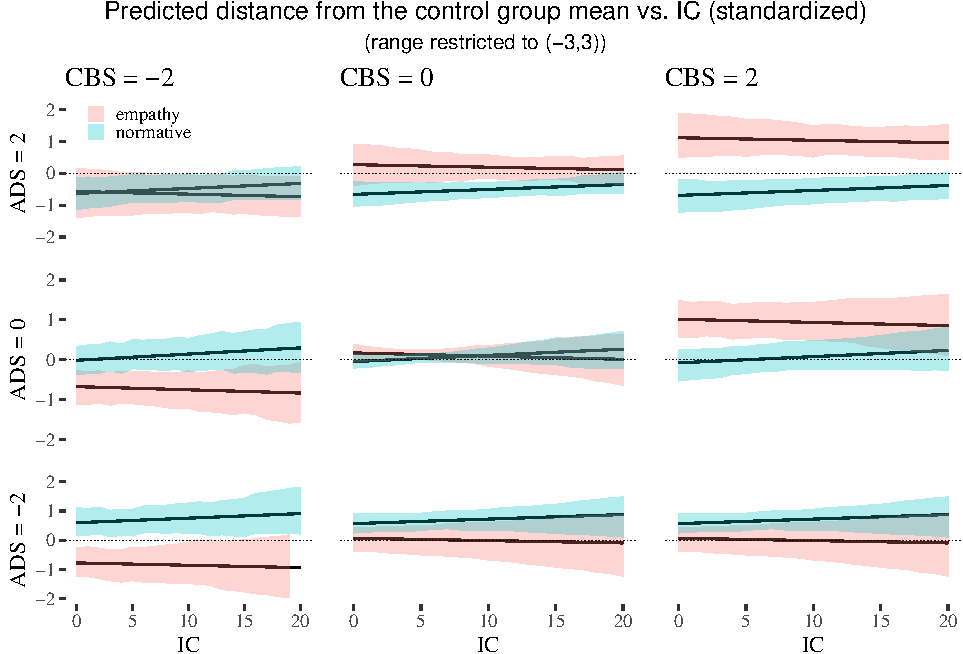
\includegraphics[width=1\linewidth]{bayesianReport3_files/figure-latex/unnamed-chunk-15-1} \end{center}
\normalsize

\hypertarget{direct-effect}{%
\section{Direct effect}\label{direct-effect}}

Models for the evaluation of direct effect need to close the indirect
causal path from the treatment variables to the output, and they do so
by conditioning on \textsf{CAS}. Again, we face model selection. We
repeat all the model structures from the previous section, except for
now, each model is extended with \textsf{CAS} as a predictor. This time
the model structure we called \textsf{tooFar} turns out to do better. We
also consider extending it with interactions between \textsf{CAS} and
\textsf{IT} and \textsf{IC} (jointly and separately), but this results
in no further improvement.

\vspace{1mm}
\footnotesize

\begin{Shaded}
\begin{Highlighting}[]
\NormalTok{nullDirect }\OtherTok{\textless{}{-}} \FunctionTok{quap}\NormalTok{(}
  \FunctionTok{alist}\NormalTok{(}
\NormalTok{    AdiffS }\SpecialCharTok{\textasciitilde{}} \FunctionTok{dnorm}\NormalTok{( mu, sigma ),}
\NormalTok{    mu }\OtherTok{\textless{}{-}}\NormalTok{ a }\SpecialCharTok{+}\NormalTok{ bCAS }\SpecialCharTok{*}\NormalTok{ CAS,}
\NormalTok{    a }\SpecialCharTok{\textasciitilde{}} \FunctionTok{dnorm}\NormalTok{ (}\DecValTok{0}\NormalTok{,}\FloatTok{0.3}\NormalTok{),}
\NormalTok{    bCAS }\SpecialCharTok{\textasciitilde{}} \FunctionTok{dnorm}\NormalTok{(}\DecValTok{0}\NormalTok{,}\FloatTok{0.3}\NormalTok{),}
\NormalTok{    sigma  }\SpecialCharTok{\textasciitilde{}} \FunctionTok{dexp}\NormalTok{(}\DecValTok{1}\NormalTok{)}
\NormalTok{  ), }
  \AttributeTok{data =}\NormalTok{ summaries  }
\NormalTok{)}

\NormalTok{ADSDirect }\OtherTok{\textless{}{-}} \FunctionTok{quap}\NormalTok{(}
  \FunctionTok{alist}\NormalTok{(}
\NormalTok{    AdiffS }\SpecialCharTok{\textasciitilde{}} \FunctionTok{dnorm}\NormalTok{( mu, sigma ),}
\NormalTok{    mu }\OtherTok{\textless{}{-}}\NormalTok{  a }\SpecialCharTok{+}\NormalTok{ bADS }\SpecialCharTok{*}\NormalTok{ ADS}\SpecialCharTok{+}\NormalTok{ bCAS }\SpecialCharTok{*}\NormalTok{ CAS,}
\NormalTok{    a }\SpecialCharTok{\textasciitilde{}} \FunctionTok{dnorm}\NormalTok{ (}\DecValTok{0}\NormalTok{,}\FloatTok{0.3}\NormalTok{),}
\NormalTok{    bADS }\SpecialCharTok{\textasciitilde{}} \FunctionTok{dnorm}\NormalTok{(}\DecValTok{0}\NormalTok{,}\FloatTok{0.3}\NormalTok{),}
\NormalTok{    bCAS }\SpecialCharTok{\textasciitilde{}} \FunctionTok{dnorm}\NormalTok{(}\DecValTok{0}\NormalTok{,}\FloatTok{0.3}\NormalTok{),}
\NormalTok{    sigma  }\SpecialCharTok{\textasciitilde{}} \FunctionTok{dexp}\NormalTok{(}\DecValTok{1}\NormalTok{)}
\NormalTok{  ), }
  \AttributeTok{data =}\NormalTok{ summaries}
\NormalTok{)}

\NormalTok{ADSICDirect }\OtherTok{\textless{}{-}} \FunctionTok{quap}\NormalTok{(}
  \FunctionTok{alist}\NormalTok{(}
\NormalTok{    AdiffS }\SpecialCharTok{\textasciitilde{}} \FunctionTok{dnorm}\NormalTok{( mu, sigma ),}
\NormalTok{    mu }\OtherTok{\textless{}{-}}\NormalTok{  a }\SpecialCharTok{+}\NormalTok{ bADS }\SpecialCharTok{*}\NormalTok{ ADS}\SpecialCharTok{+}\NormalTok{ bIC }\SpecialCharTok{*}\NormalTok{ IC}\SpecialCharTok{+}\NormalTok{ bCAS }\SpecialCharTok{*}\NormalTok{ CAS,}
\NormalTok{    a }\SpecialCharTok{\textasciitilde{}} \FunctionTok{dnorm}\NormalTok{ (}\DecValTok{0}\NormalTok{,}\FloatTok{0.3}\NormalTok{),}
\NormalTok{    bADS }\SpecialCharTok{\textasciitilde{}} \FunctionTok{dnorm}\NormalTok{(}\DecValTok{0}\NormalTok{,}\FloatTok{0.3}\NormalTok{),}
\NormalTok{    bIC }\SpecialCharTok{\textasciitilde{}} \FunctionTok{dnorm}\NormalTok{(}\DecValTok{0}\NormalTok{,}\FloatTok{0.3}\NormalTok{),}
\NormalTok{    bCAS }\SpecialCharTok{\textasciitilde{}} \FunctionTok{dnorm}\NormalTok{(}\DecValTok{0}\NormalTok{,}\FloatTok{0.3}\NormalTok{),}
\NormalTok{    sigma  }\SpecialCharTok{\textasciitilde{}} \FunctionTok{dexp}\NormalTok{(}\DecValTok{1}\NormalTok{)}
\NormalTok{  ), }
  \AttributeTok{data =}\NormalTok{ summaries}
\NormalTok{)}

\NormalTok{ITDirect }\OtherTok{\textless{}{-}} \FunctionTok{quap}\NormalTok{(}
  \FunctionTok{alist}\NormalTok{(}
\NormalTok{    AdiffS }\SpecialCharTok{\textasciitilde{}} \FunctionTok{dnorm}\NormalTok{( mu, sigma ),}
\NormalTok{    mu }\OtherTok{\textless{}{-}}\NormalTok{  bIT[groupID] }\SpecialCharTok{+}\NormalTok{ bCAS }\SpecialCharTok{*}\NormalTok{ CAS,}
\NormalTok{    bIT[groupID] }\SpecialCharTok{\textasciitilde{}} \FunctionTok{dnorm}\NormalTok{(}\DecValTok{0}\NormalTok{,.}\DecValTok{3}\NormalTok{),}
\NormalTok{    bCAS }\SpecialCharTok{\textasciitilde{}} \FunctionTok{dnorm}\NormalTok{(}\DecValTok{0}\NormalTok{,}\FloatTok{0.3}\NormalTok{),}
\NormalTok{    sigma  }\SpecialCharTok{\textasciitilde{}} \FunctionTok{dexp}\NormalTok{(}\DecValTok{1}\NormalTok{)}
\NormalTok{  ), }
  \AttributeTok{data =}\NormalTok{ summaries}
\NormalTok{)}

\NormalTok{ADSITDirect }\OtherTok{\textless{}{-}} \FunctionTok{quap}\NormalTok{(}
  \FunctionTok{alist}\NormalTok{(}
\NormalTok{    AdiffS }\SpecialCharTok{\textasciitilde{}} \FunctionTok{dnorm}\NormalTok{( mu, sigma ),}
\NormalTok{    mu }\OtherTok{\textless{}{-}}\NormalTok{ a }\SpecialCharTok{+}\NormalTok{ bADS }\SpecialCharTok{*}\NormalTok{ ADS }\SpecialCharTok{+}\NormalTok{  bIT[groupID]}\SpecialCharTok{+}\NormalTok{ bCAS }\SpecialCharTok{*}\NormalTok{ CAS,}
\NormalTok{    a }\SpecialCharTok{\textasciitilde{}} \FunctionTok{dnorm}\NormalTok{ (}\DecValTok{0}\NormalTok{,}\FloatTok{0.3}\NormalTok{),}
\NormalTok{    bADS }\SpecialCharTok{\textasciitilde{}} \FunctionTok{dnorm}\NormalTok{(}\DecValTok{0}\NormalTok{,.}\DecValTok{3}\NormalTok{),}
\NormalTok{    bCAS }\SpecialCharTok{\textasciitilde{}} \FunctionTok{dnorm}\NormalTok{(}\DecValTok{0}\NormalTok{,}\FloatTok{0.3}\NormalTok{),}
\NormalTok{    bIT[groupID] }\SpecialCharTok{\textasciitilde{}} \FunctionTok{dnorm}\NormalTok{(}\DecValTok{0}\NormalTok{,.}\DecValTok{3}\NormalTok{),}
\NormalTok{    sigma  }\SpecialCharTok{\textasciitilde{}} \FunctionTok{dexp}\NormalTok{(}\DecValTok{1}\NormalTok{)}
\NormalTok{  ), }
  \AttributeTok{data =}\NormalTok{ summaries}
\NormalTok{)}


\NormalTok{ADSITICDirect }\OtherTok{\textless{}{-}} \FunctionTok{quap}\NormalTok{(}
  \FunctionTok{alist}\NormalTok{(}
\NormalTok{    AdiffS }\SpecialCharTok{\textasciitilde{}} \FunctionTok{dnorm}\NormalTok{( mu, sigma ),}
\NormalTok{    mu }\OtherTok{\textless{}{-}}\NormalTok{ a }\SpecialCharTok{+}\NormalTok{ bADS }\SpecialCharTok{*}\NormalTok{ ADS }\SpecialCharTok{+}\NormalTok{  bIT[groupID] }\SpecialCharTok{+}\NormalTok{ bIC }\SpecialCharTok{*}\NormalTok{ IC}\SpecialCharTok{+}\NormalTok{ bCAS }\SpecialCharTok{*}\NormalTok{ CAS,}
\NormalTok{    a }\SpecialCharTok{\textasciitilde{}} \FunctionTok{dnorm}\NormalTok{ (}\DecValTok{0}\NormalTok{,}\FloatTok{0.3}\NormalTok{),}
\NormalTok{    bADS }\SpecialCharTok{\textasciitilde{}} \FunctionTok{dnorm}\NormalTok{(}\DecValTok{0}\NormalTok{,.}\DecValTok{3}\NormalTok{),}
\NormalTok{    bCAS }\SpecialCharTok{\textasciitilde{}} \FunctionTok{dnorm}\NormalTok{(}\DecValTok{0}\NormalTok{,}\FloatTok{0.3}\NormalTok{),}
\NormalTok{    bIT[groupID] }\SpecialCharTok{\textasciitilde{}} \FunctionTok{dnorm}\NormalTok{(}\DecValTok{0}\NormalTok{,.}\DecValTok{3}\NormalTok{),}
\NormalTok{    bIC }\SpecialCharTok{\textasciitilde{}} \FunctionTok{dnorm}\NormalTok{(}\DecValTok{0}\NormalTok{,.}\DecValTok{3}\NormalTok{),}
\NormalTok{    sigma  }\SpecialCharTok{\textasciitilde{}} \FunctionTok{dexp}\NormalTok{(}\DecValTok{1}\NormalTok{)}
\NormalTok{  ), }
  \AttributeTok{data =}\NormalTok{ summaries}
\NormalTok{)}


\NormalTok{ADSITIC\_ADSICDirect }\OtherTok{\textless{}{-}} \FunctionTok{quap}\NormalTok{(}
  \FunctionTok{alist}\NormalTok{(}
\NormalTok{    AdiffS }\SpecialCharTok{\textasciitilde{}} \FunctionTok{dnorm}\NormalTok{( mu, sigma ),}
\NormalTok{    mu }\OtherTok{\textless{}{-}}\NormalTok{ a }\SpecialCharTok{+}\NormalTok{ bADS }\SpecialCharTok{*}\NormalTok{ ADS }\SpecialCharTok{+}\NormalTok{  bIT[groupID] }\SpecialCharTok{+}\NormalTok{ bIC }\SpecialCharTok{*}\NormalTok{ IC }\SpecialCharTok{+}\NormalTok{ bADSIC }\SpecialCharTok{*}\NormalTok{ ADS }\SpecialCharTok{*}\NormalTok{ IC}\SpecialCharTok{+}\NormalTok{ bCAS }\SpecialCharTok{*}\NormalTok{ CAS,}
\NormalTok{    a }\SpecialCharTok{\textasciitilde{}} \FunctionTok{dnorm}\NormalTok{ (}\DecValTok{0}\NormalTok{,}\FloatTok{0.3}\NormalTok{),}
\NormalTok{    bADS }\SpecialCharTok{\textasciitilde{}} \FunctionTok{dnorm}\NormalTok{(}\DecValTok{0}\NormalTok{,.}\DecValTok{3}\NormalTok{),}
\NormalTok{    bCAS }\SpecialCharTok{\textasciitilde{}} \FunctionTok{dnorm}\NormalTok{(}\DecValTok{0}\NormalTok{,}\FloatTok{0.3}\NormalTok{),}
\NormalTok{    bADSIC }\SpecialCharTok{\textasciitilde{}} \FunctionTok{dnorm}\NormalTok{(}\DecValTok{0}\NormalTok{,.}\DecValTok{3}\NormalTok{),}
\NormalTok{    bIT[groupID] }\SpecialCharTok{\textasciitilde{}} \FunctionTok{dnorm}\NormalTok{(}\DecValTok{0}\NormalTok{,.}\DecValTok{3}\NormalTok{),}
\NormalTok{    bIC }\SpecialCharTok{\textasciitilde{}} \FunctionTok{dnorm}\NormalTok{(}\DecValTok{0}\NormalTok{,.}\DecValTok{3}\NormalTok{),}
\NormalTok{    sigma  }\SpecialCharTok{\textasciitilde{}} \FunctionTok{dexp}\NormalTok{(}\DecValTok{1}\NormalTok{)}
\NormalTok{  ), }
  \AttributeTok{data =}\NormalTok{ summaries}
\NormalTok{)}


\NormalTok{ADSITIC\_ADSIC\_ADSITDirect }\OtherTok{\textless{}{-}} \FunctionTok{quap}\NormalTok{(}
  \FunctionTok{alist}\NormalTok{(}
\NormalTok{    AdiffS }\SpecialCharTok{\textasciitilde{}} \FunctionTok{dnorm}\NormalTok{( mu, sigma ),}
\NormalTok{    mu }\OtherTok{\textless{}{-}}\NormalTok{ a }\SpecialCharTok{+}\NormalTok{ bADS[groupID] }\SpecialCharTok{*}\NormalTok{ ADS }\SpecialCharTok{+}\NormalTok{  bIT[groupID] }\SpecialCharTok{+}\NormalTok{ bIC }\SpecialCharTok{*}\NormalTok{ IC }\SpecialCharTok{+}\NormalTok{ bADSIC }\SpecialCharTok{*}\NormalTok{ ADS }\SpecialCharTok{*}\NormalTok{ IC}\SpecialCharTok{+}\NormalTok{ bCAS }\SpecialCharTok{*}\NormalTok{ CAS,}
\NormalTok{    a }\SpecialCharTok{\textasciitilde{}} \FunctionTok{dnorm}\NormalTok{ (}\DecValTok{0}\NormalTok{,}\FloatTok{0.3}\NormalTok{),}
\NormalTok{    bADS[groupID] }\SpecialCharTok{\textasciitilde{}} \FunctionTok{dnorm}\NormalTok{(}\DecValTok{0}\NormalTok{,.}\DecValTok{3}\NormalTok{),}
\NormalTok{    bADSIC }\SpecialCharTok{\textasciitilde{}} \FunctionTok{dnorm}\NormalTok{(}\DecValTok{0}\NormalTok{,.}\DecValTok{3}\NormalTok{),}
\NormalTok{    bCAS }\SpecialCharTok{\textasciitilde{}} \FunctionTok{dnorm}\NormalTok{(}\DecValTok{0}\NormalTok{,}\FloatTok{0.3}\NormalTok{),}
\NormalTok{    bIT[groupID] }\SpecialCharTok{\textasciitilde{}} \FunctionTok{dnorm}\NormalTok{(}\DecValTok{0}\NormalTok{,.}\DecValTok{3}\NormalTok{),}
\NormalTok{    bIC }\SpecialCharTok{\textasciitilde{}} \FunctionTok{dnorm}\NormalTok{(}\DecValTok{0}\NormalTok{,.}\DecValTok{3}\NormalTok{),}
\NormalTok{    sigma  }\SpecialCharTok{\textasciitilde{}} \FunctionTok{dexp}\NormalTok{(}\DecValTok{1}\NormalTok{)}
\NormalTok{  ), }
  \AttributeTok{data =}\NormalTok{ summaries}
\NormalTok{)}


\NormalTok{ADSIT\_ADSITDirect }\OtherTok{\textless{}{-}} \FunctionTok{quap}\NormalTok{(}
  \FunctionTok{alist}\NormalTok{(}
\NormalTok{    AdiffS }\SpecialCharTok{\textasciitilde{}} \FunctionTok{dnorm}\NormalTok{( mu, sigma ),}
\NormalTok{    mu }\OtherTok{\textless{}{-}}\NormalTok{ a }\SpecialCharTok{+}\NormalTok{ bADS[groupID] }\SpecialCharTok{*}\NormalTok{ ADS }\SpecialCharTok{+}\NormalTok{  bIT[groupID] }\SpecialCharTok{+}\NormalTok{ bCAS }\SpecialCharTok{*}\NormalTok{ CAS,}
\NormalTok{    a }\SpecialCharTok{\textasciitilde{}} \FunctionTok{dnorm}\NormalTok{ (}\DecValTok{0}\NormalTok{,}\FloatTok{0.3}\NormalTok{),}
\NormalTok{    bADS[groupID] }\SpecialCharTok{\textasciitilde{}} \FunctionTok{dnorm}\NormalTok{(}\DecValTok{0}\NormalTok{,.}\DecValTok{3}\NormalTok{),}
    \CommentTok{\#bADSIC \textasciitilde{} dnorm(0,.5),}
\NormalTok{    bIT[groupID] }\SpecialCharTok{\textasciitilde{}} \FunctionTok{dnorm}\NormalTok{(}\DecValTok{0}\NormalTok{,.}\DecValTok{3}\NormalTok{),}
    \CommentTok{\#bIC \textasciitilde{} dnorm(0,.5),}
\NormalTok{    bCAS }\SpecialCharTok{\textasciitilde{}} \FunctionTok{dnorm}\NormalTok{(}\DecValTok{0}\NormalTok{,}\FloatTok{0.3}\NormalTok{),}
\NormalTok{    sigma  }\SpecialCharTok{\textasciitilde{}} \FunctionTok{dexp}\NormalTok{(}\DecValTok{1}\NormalTok{)}
\NormalTok{  ), }
  \AttributeTok{data =}\NormalTok{ summaries}
\NormalTok{)}


\NormalTok{ADSITIC\_ADSIT\_ITIC\_ADSICDirect }\OtherTok{\textless{}{-}} \FunctionTok{quap}\NormalTok{(}
  \FunctionTok{alist}\NormalTok{(}
\NormalTok{    AdiffS }\SpecialCharTok{\textasciitilde{}} \FunctionTok{dnorm}\NormalTok{( mu, sigma ),}
\NormalTok{    mu }\OtherTok{\textless{}{-}}\NormalTok{ a }\SpecialCharTok{+}\NormalTok{ bADS[groupID] }\SpecialCharTok{*}\NormalTok{ ADS }\SpecialCharTok{+}\NormalTok{  bIT[groupID] }\SpecialCharTok{+}\NormalTok{ bIC[groupID] }\SpecialCharTok{*}\NormalTok{ IC }\SpecialCharTok{+}
\NormalTok{      bADSIC }\SpecialCharTok{*}\NormalTok{ ADS }\SpecialCharTok{*}\NormalTok{ IC }\SpecialCharTok{+}\NormalTok{ bCAS }\SpecialCharTok{*}\NormalTok{ CAS,}
\NormalTok{    a }\SpecialCharTok{\textasciitilde{}} \FunctionTok{dnorm}\NormalTok{ (}\DecValTok{0}\NormalTok{,}\FloatTok{0.3}\NormalTok{),}
\NormalTok{    bADS[groupID] }\SpecialCharTok{\textasciitilde{}} \FunctionTok{dnorm}\NormalTok{(}\DecValTok{0}\NormalTok{,.}\DecValTok{3}\NormalTok{),}
\NormalTok{    bADSIC }\SpecialCharTok{\textasciitilde{}} \FunctionTok{dnorm}\NormalTok{(}\DecValTok{0}\NormalTok{,.}\DecValTok{3}\NormalTok{),}
\NormalTok{    bCAS }\SpecialCharTok{\textasciitilde{}} \FunctionTok{dnorm}\NormalTok{(}\DecValTok{0}\NormalTok{,}\FloatTok{0.3}\NormalTok{),}
\NormalTok{    bIT[groupID] }\SpecialCharTok{\textasciitilde{}} \FunctionTok{dnorm}\NormalTok{(}\DecValTok{0}\NormalTok{,.}\DecValTok{3}\NormalTok{),}
\NormalTok{    bIC[groupID] }\SpecialCharTok{\textasciitilde{}} \FunctionTok{dnorm}\NormalTok{(}\DecValTok{0}\NormalTok{,.}\DecValTok{3}\NormalTok{),}
\NormalTok{    sigma  }\SpecialCharTok{\textasciitilde{}} \FunctionTok{dexp}\NormalTok{(}\DecValTok{1}\NormalTok{)}
\NormalTok{  ), }
  \AttributeTok{data =}\NormalTok{ summaries}
\NormalTok{)}


\NormalTok{ADSITICCBS\_ITIC\_ADSICDirect }\OtherTok{\textless{}{-}} \FunctionTok{quap}\NormalTok{(}
  \FunctionTok{alist}\NormalTok{(}
\NormalTok{    AdiffS }\SpecialCharTok{\textasciitilde{}} \FunctionTok{dnorm}\NormalTok{( mu, sigma ),}
\NormalTok{    mu }\OtherTok{\textless{}{-}}\NormalTok{ a }\SpecialCharTok{+}\NormalTok{ bADS[groupID] }\SpecialCharTok{*}\NormalTok{ ADS }\SpecialCharTok{+}\NormalTok{  bIT[groupID] }\SpecialCharTok{+}\NormalTok{ bIC[groupID] }\SpecialCharTok{*}\NormalTok{ IC }\SpecialCharTok{+} 
\NormalTok{      bADSIC }\SpecialCharTok{*}\NormalTok{ ADS }\SpecialCharTok{*}\NormalTok{ IC}\SpecialCharTok{+}\NormalTok{ bCBS }\SpecialCharTok{*}\NormalTok{CBS }\SpecialCharTok{+}\NormalTok{ bCAS }\SpecialCharTok{*}\NormalTok{ CAS,}
\NormalTok{    a }\SpecialCharTok{\textasciitilde{}} \FunctionTok{dnorm}\NormalTok{ (}\DecValTok{0}\NormalTok{,}\FloatTok{0.3}\NormalTok{),}
\NormalTok{    bADS[groupID] }\SpecialCharTok{\textasciitilde{}} \FunctionTok{dnorm}\NormalTok{(}\DecValTok{0}\NormalTok{,.}\DecValTok{3}\NormalTok{),}
\NormalTok{    bADSIC }\SpecialCharTok{\textasciitilde{}} \FunctionTok{dnorm}\NormalTok{(}\DecValTok{0}\NormalTok{,.}\DecValTok{3}\NormalTok{),}
\NormalTok{    bCBS }\SpecialCharTok{\textasciitilde{}} \FunctionTok{dnorm}\NormalTok{(}\DecValTok{0}\NormalTok{,.}\DecValTok{3}\NormalTok{),}
\NormalTok{    bCAS }\SpecialCharTok{\textasciitilde{}} \FunctionTok{dnorm}\NormalTok{(}\DecValTok{0}\NormalTok{,}\FloatTok{0.3}\NormalTok{),}
\NormalTok{    bIT[groupID] }\SpecialCharTok{\textasciitilde{}} \FunctionTok{dnorm}\NormalTok{(}\DecValTok{0}\NormalTok{,.}\DecValTok{3}\NormalTok{),}
\NormalTok{    bIC[groupID] }\SpecialCharTok{\textasciitilde{}} \FunctionTok{dnorm}\NormalTok{(}\DecValTok{0}\NormalTok{,.}\DecValTok{3}\NormalTok{),}
\NormalTok{    sigma  }\SpecialCharTok{\textasciitilde{}} \FunctionTok{dexp}\NormalTok{(}\DecValTok{1}\NormalTok{)}
\NormalTok{  ), }
  \AttributeTok{data =}\NormalTok{ summaries}
\NormalTok{)}


\NormalTok{FinalDirect }\OtherTok{\textless{}{-}} \FunctionTok{quap}\NormalTok{(}
  \FunctionTok{alist}\NormalTok{(}
\NormalTok{    AdiffS }\SpecialCharTok{\textasciitilde{}} \FunctionTok{dnorm}\NormalTok{( mu, sigma ),}
\NormalTok{    mu }\OtherTok{\textless{}{-}}\NormalTok{ a }\SpecialCharTok{+}\NormalTok{ bADS[groupID] }\SpecialCharTok{*}\NormalTok{ ADS }\SpecialCharTok{+}\NormalTok{  bIT[groupID] }\SpecialCharTok{+}\NormalTok{ bIC[groupID] }\SpecialCharTok{*}\NormalTok{ IC }\SpecialCharTok{+} 
\NormalTok{      bADSIC }\SpecialCharTok{*}\NormalTok{ ADS }\SpecialCharTok{*}\NormalTok{ IC}\SpecialCharTok{+}\NormalTok{ bCBS[groupID] }\SpecialCharTok{*}\NormalTok{CBS }\SpecialCharTok{+}\NormalTok{ bCAS }\SpecialCharTok{*}\NormalTok{ CAS,}
\NormalTok{    a }\SpecialCharTok{\textasciitilde{}} \FunctionTok{dnorm}\NormalTok{ (}\DecValTok{0}\NormalTok{,}\FloatTok{0.3}\NormalTok{),}
\NormalTok{    bADS[groupID] }\SpecialCharTok{\textasciitilde{}} \FunctionTok{dnorm}\NormalTok{(}\DecValTok{0}\NormalTok{,.}\DecValTok{3}\NormalTok{),}
\NormalTok{    bADSIC }\SpecialCharTok{\textasciitilde{}} \FunctionTok{dnorm}\NormalTok{(}\DecValTok{0}\NormalTok{,.}\DecValTok{3}\NormalTok{),}
\NormalTok{    bCAS }\SpecialCharTok{\textasciitilde{}} \FunctionTok{dnorm}\NormalTok{(}\DecValTok{0}\NormalTok{,}\FloatTok{0.3}\NormalTok{),}
\NormalTok{    bCBS[groupID] }\SpecialCharTok{\textasciitilde{}} \FunctionTok{dnorm}\NormalTok{(}\DecValTok{0}\NormalTok{,.}\DecValTok{3}\NormalTok{),}
\NormalTok{    bIT[groupID] }\SpecialCharTok{\textasciitilde{}} \FunctionTok{dnorm}\NormalTok{(}\DecValTok{0}\NormalTok{,.}\DecValTok{3}\NormalTok{),}
\NormalTok{    bIC[groupID] }\SpecialCharTok{\textasciitilde{}} \FunctionTok{dnorm}\NormalTok{(}\DecValTok{0}\NormalTok{,.}\DecValTok{3}\NormalTok{),}
\NormalTok{    sigma  }\SpecialCharTok{\textasciitilde{}} \FunctionTok{dexp}\NormalTok{(}\DecValTok{1}\NormalTok{)}
\NormalTok{  ), }
  \AttributeTok{data =}\NormalTok{ summaries}
\NormalTok{)}



\NormalTok{tooFarDirect }\OtherTok{\textless{}{-}} \FunctionTok{quap}\NormalTok{(}
  \FunctionTok{alist}\NormalTok{(}
\NormalTok{    AdiffS }\SpecialCharTok{\textasciitilde{}} \FunctionTok{dnorm}\NormalTok{( mu, sigma ),}
\NormalTok{    mu }\OtherTok{\textless{}{-}}\NormalTok{ a }\SpecialCharTok{+}\NormalTok{ bADS[groupID] }\SpecialCharTok{*}\NormalTok{ ADS }\SpecialCharTok{+}\NormalTok{  bIT[groupID] }\SpecialCharTok{+}\NormalTok{ bIC[groupID] }\SpecialCharTok{*}\NormalTok{ IC }\SpecialCharTok{+} 
\NormalTok{      bADSIC }\SpecialCharTok{*}\NormalTok{ ADS }\SpecialCharTok{*}\NormalTok{ IC}\SpecialCharTok{+}\NormalTok{ bCBS[groupID] }\SpecialCharTok{*}\NormalTok{CBS }\SpecialCharTok{+}\NormalTok{ bCBSIC }\SpecialCharTok{*}\NormalTok{ CBS }\SpecialCharTok{*}\NormalTok{ IC }\SpecialCharTok{+}\NormalTok{ bCAS }\SpecialCharTok{*}\NormalTok{ CAS, }
\NormalTok{    a }\SpecialCharTok{\textasciitilde{}} \FunctionTok{dnorm}\NormalTok{ (}\DecValTok{0}\NormalTok{,}\FloatTok{0.3}\NormalTok{),}
\NormalTok{    bADS[groupID] }\SpecialCharTok{\textasciitilde{}} \FunctionTok{dnorm}\NormalTok{(}\DecValTok{0}\NormalTok{,.}\DecValTok{3}\NormalTok{),}
\NormalTok{    bADSIC }\SpecialCharTok{\textasciitilde{}} \FunctionTok{dnorm}\NormalTok{(}\DecValTok{0}\NormalTok{,.}\DecValTok{3}\NormalTok{),}
\NormalTok{    bCAS }\SpecialCharTok{\textasciitilde{}} \FunctionTok{dnorm}\NormalTok{(}\DecValTok{0}\NormalTok{,}\FloatTok{0.3}\NormalTok{),}
\NormalTok{    bCBS[groupID] }\SpecialCharTok{\textasciitilde{}} \FunctionTok{dnorm}\NormalTok{(}\DecValTok{0}\NormalTok{,.}\DecValTok{3}\NormalTok{),}
\NormalTok{    bIT[groupID] }\SpecialCharTok{\textasciitilde{}} \FunctionTok{dnorm}\NormalTok{(}\DecValTok{0}\NormalTok{,.}\DecValTok{3}\NormalTok{),}
\NormalTok{    bIC[groupID] }\SpecialCharTok{\textasciitilde{}} \FunctionTok{dnorm}\NormalTok{(}\DecValTok{0}\NormalTok{,.}\DecValTok{3}\NormalTok{),}
\NormalTok{    bCBSIC }\SpecialCharTok{\textasciitilde{}} \FunctionTok{dnorm}\NormalTok{(}\DecValTok{0}\NormalTok{, .}\DecValTok{3}\NormalTok{),}
\NormalTok{    sigma  }\SpecialCharTok{\textasciitilde{}} \FunctionTok{dexp}\NormalTok{(}\DecValTok{1}\NormalTok{)}
\NormalTok{  ), }
  \AttributeTok{data =}\NormalTok{ summaries}
\NormalTok{)}




\NormalTok{tooFarDirect\_CASIT }\OtherTok{\textless{}{-}} \FunctionTok{quap}\NormalTok{(}
  \FunctionTok{alist}\NormalTok{(}
\NormalTok{    AdiffS }\SpecialCharTok{\textasciitilde{}} \FunctionTok{dnorm}\NormalTok{( mu, sigma ),}
\NormalTok{    mu }\OtherTok{\textless{}{-}}\NormalTok{ a }\SpecialCharTok{+}\NormalTok{ bADS[groupID] }\SpecialCharTok{*}\NormalTok{ ADS }\SpecialCharTok{+}\NormalTok{  bIT[groupID] }\SpecialCharTok{+}\NormalTok{ bIC[groupID] }\SpecialCharTok{*}\NormalTok{ IC }\SpecialCharTok{+} 
\NormalTok{      bADSIC }\SpecialCharTok{*}\NormalTok{ ADS }\SpecialCharTok{*}\NormalTok{ IC}\SpecialCharTok{+}\NormalTok{ bCBS[groupID] }\SpecialCharTok{*}\NormalTok{CBS }\SpecialCharTok{+}\NormalTok{ bCBSIC }\SpecialCharTok{*}\NormalTok{ CBS }\SpecialCharTok{*}\NormalTok{ IC }\SpecialCharTok{+}\NormalTok{ bCAS[groupID] }\SpecialCharTok{*}\NormalTok{ CAS, }
\NormalTok{    a }\SpecialCharTok{\textasciitilde{}} \FunctionTok{dnorm}\NormalTok{ (}\DecValTok{0}\NormalTok{,}\FloatTok{0.3}\NormalTok{),}
\NormalTok{    bADS[groupID] }\SpecialCharTok{\textasciitilde{}} \FunctionTok{dnorm}\NormalTok{(}\DecValTok{0}\NormalTok{,.}\DecValTok{3}\NormalTok{),}
\NormalTok{    bADSIC }\SpecialCharTok{\textasciitilde{}} \FunctionTok{dnorm}\NormalTok{(}\DecValTok{0}\NormalTok{,.}\DecValTok{3}\NormalTok{),}
\NormalTok{    bCAS[groupID] }\SpecialCharTok{\textasciitilde{}} \FunctionTok{dnorm}\NormalTok{(}\DecValTok{0}\NormalTok{,}\FloatTok{0.3}\NormalTok{),}
\NormalTok{    bCBS[groupID] }\SpecialCharTok{\textasciitilde{}} \FunctionTok{dnorm}\NormalTok{(}\DecValTok{0}\NormalTok{,.}\DecValTok{3}\NormalTok{),}
\NormalTok{    bIT[groupID] }\SpecialCharTok{\textasciitilde{}} \FunctionTok{dnorm}\NormalTok{(}\DecValTok{0}\NormalTok{,.}\DecValTok{3}\NormalTok{),}
\NormalTok{    bIC[groupID] }\SpecialCharTok{\textasciitilde{}} \FunctionTok{dnorm}\NormalTok{(}\DecValTok{0}\NormalTok{,.}\DecValTok{3}\NormalTok{),}
\NormalTok{    bCBSIC }\SpecialCharTok{\textasciitilde{}} \FunctionTok{dnorm}\NormalTok{(}\DecValTok{0}\NormalTok{, .}\DecValTok{3}\NormalTok{),}
\NormalTok{    sigma  }\SpecialCharTok{\textasciitilde{}} \FunctionTok{dexp}\NormalTok{(}\DecValTok{1}\NormalTok{)}
\NormalTok{  ), }
  \AttributeTok{data =}\NormalTok{ summaries}
\NormalTok{)}



\NormalTok{tooFarDirect\_CASIC }\OtherTok{\textless{}{-}} \FunctionTok{quap}\NormalTok{(}
  \FunctionTok{alist}\NormalTok{(}
\NormalTok{    AdiffS }\SpecialCharTok{\textasciitilde{}} \FunctionTok{dnorm}\NormalTok{( mu, sigma ),}
\NormalTok{    mu }\OtherTok{\textless{}{-}}\NormalTok{ a }\SpecialCharTok{+}\NormalTok{ bADS[groupID] }\SpecialCharTok{*}\NormalTok{ ADS }\SpecialCharTok{+}\NormalTok{  bIT[groupID] }\SpecialCharTok{+}\NormalTok{ bIC[groupID] }\SpecialCharTok{*}\NormalTok{ IC }\SpecialCharTok{+} 
\NormalTok{      bADSIC }\SpecialCharTok{*}\NormalTok{ ADS }\SpecialCharTok{*}\NormalTok{ IC}\SpecialCharTok{+}\NormalTok{ bCBS[groupID] }\SpecialCharTok{*}\NormalTok{CBS }\SpecialCharTok{+}\NormalTok{ bCBSIC }\SpecialCharTok{*}\NormalTok{ CBS }\SpecialCharTok{*}\NormalTok{ IC }\SpecialCharTok{+}\NormalTok{ bCAS }\SpecialCharTok{*}\NormalTok{ CAS }\SpecialCharTok{+}\NormalTok{ bCASIC }\SpecialCharTok{*}\NormalTok{ CAS }\SpecialCharTok{*}\NormalTok{ IC, }
\NormalTok{    a }\SpecialCharTok{\textasciitilde{}} \FunctionTok{dnorm}\NormalTok{ (}\DecValTok{0}\NormalTok{,}\FloatTok{0.3}\NormalTok{),}
\NormalTok{    bADS[groupID] }\SpecialCharTok{\textasciitilde{}} \FunctionTok{dnorm}\NormalTok{(}\DecValTok{0}\NormalTok{,.}\DecValTok{3}\NormalTok{),}
\NormalTok{    bADSIC }\SpecialCharTok{\textasciitilde{}} \FunctionTok{dnorm}\NormalTok{(}\DecValTok{0}\NormalTok{,.}\DecValTok{3}\NormalTok{),}
\NormalTok{    bCAS }\SpecialCharTok{\textasciitilde{}} \FunctionTok{dnorm}\NormalTok{(}\DecValTok{0}\NormalTok{,}\FloatTok{0.3}\NormalTok{),}
\NormalTok{    bCASIC }\SpecialCharTok{\textasciitilde{}} \FunctionTok{dnorm}\NormalTok{(}\DecValTok{0}\NormalTok{,}\FloatTok{0.3}\NormalTok{),}
\NormalTok{    bCBS[groupID] }\SpecialCharTok{\textasciitilde{}} \FunctionTok{dnorm}\NormalTok{(}\DecValTok{0}\NormalTok{,.}\DecValTok{3}\NormalTok{),}
\NormalTok{    bIT[groupID] }\SpecialCharTok{\textasciitilde{}} \FunctionTok{dnorm}\NormalTok{(}\DecValTok{0}\NormalTok{,.}\DecValTok{3}\NormalTok{),}
\NormalTok{    bIC[groupID] }\SpecialCharTok{\textasciitilde{}} \FunctionTok{dnorm}\NormalTok{(}\DecValTok{0}\NormalTok{,.}\DecValTok{3}\NormalTok{),}
\NormalTok{    bCBSIC }\SpecialCharTok{\textasciitilde{}} \FunctionTok{dnorm}\NormalTok{(}\DecValTok{0}\NormalTok{, .}\DecValTok{3}\NormalTok{),}
\NormalTok{    sigma  }\SpecialCharTok{\textasciitilde{}} \FunctionTok{dexp}\NormalTok{(}\DecValTok{1}\NormalTok{)}
\NormalTok{  ), }
  \AttributeTok{data =}\NormalTok{ summaries}
\NormalTok{)}


\NormalTok{tooFarDirect\_CASIC\_CASIT }\OtherTok{\textless{}{-}} \FunctionTok{quap}\NormalTok{(}
  \FunctionTok{alist}\NormalTok{(}
\NormalTok{    AdiffS }\SpecialCharTok{\textasciitilde{}} \FunctionTok{dnorm}\NormalTok{( mu, sigma ),}
\NormalTok{    mu }\OtherTok{\textless{}{-}}\NormalTok{ a }\SpecialCharTok{+}\NormalTok{ bADS[groupID] }\SpecialCharTok{*}\NormalTok{ ADS }\SpecialCharTok{+}\NormalTok{  bIT[groupID] }\SpecialCharTok{+}\NormalTok{ bIC[groupID] }\SpecialCharTok{*}\NormalTok{ IC }\SpecialCharTok{+} 
\NormalTok{      bADSIC }\SpecialCharTok{*}\NormalTok{ ADS }\SpecialCharTok{*}\NormalTok{ IC}\SpecialCharTok{+}\NormalTok{ bCBS[groupID] }\SpecialCharTok{*}\NormalTok{CBS }\SpecialCharTok{+}\NormalTok{ bCBSIC }\SpecialCharTok{*}\NormalTok{ CBS }\SpecialCharTok{*}\NormalTok{ IC }\SpecialCharTok{+}\NormalTok{ bCAS[groupID] }\SpecialCharTok{*}\NormalTok{ CAS }\SpecialCharTok{+}\NormalTok{ bCASIC }\SpecialCharTok{*}\NormalTok{ CAS }\SpecialCharTok{*}\NormalTok{ IC, }
\NormalTok{    a }\SpecialCharTok{\textasciitilde{}} \FunctionTok{dnorm}\NormalTok{ (}\DecValTok{0}\NormalTok{,}\FloatTok{0.3}\NormalTok{),}
\NormalTok{    bADS[groupID] }\SpecialCharTok{\textasciitilde{}} \FunctionTok{dnorm}\NormalTok{(}\DecValTok{0}\NormalTok{,.}\DecValTok{3}\NormalTok{),}
\NormalTok{    bADSIC }\SpecialCharTok{\textasciitilde{}} \FunctionTok{dnorm}\NormalTok{(}\DecValTok{0}\NormalTok{,.}\DecValTok{3}\NormalTok{),}
\NormalTok{    bCAS[groupID] }\SpecialCharTok{\textasciitilde{}} \FunctionTok{dnorm}\NormalTok{(}\DecValTok{0}\NormalTok{,}\FloatTok{0.3}\NormalTok{),}
\NormalTok{    bCASIC }\SpecialCharTok{\textasciitilde{}} \FunctionTok{dnorm}\NormalTok{(}\DecValTok{0}\NormalTok{,}\FloatTok{0.3}\NormalTok{),}
\NormalTok{    bCBS[groupID] }\SpecialCharTok{\textasciitilde{}} \FunctionTok{dnorm}\NormalTok{(}\DecValTok{0}\NormalTok{,.}\DecValTok{3}\NormalTok{),}
\NormalTok{    bIT[groupID] }\SpecialCharTok{\textasciitilde{}} \FunctionTok{dnorm}\NormalTok{(}\DecValTok{0}\NormalTok{,.}\DecValTok{3}\NormalTok{),}
\NormalTok{    bIC[groupID] }\SpecialCharTok{\textasciitilde{}} \FunctionTok{dnorm}\NormalTok{(}\DecValTok{0}\NormalTok{,.}\DecValTok{3}\NormalTok{),}
\NormalTok{    bCBSIC }\SpecialCharTok{\textasciitilde{}} \FunctionTok{dnorm}\NormalTok{(}\DecValTok{0}\NormalTok{, .}\DecValTok{3}\NormalTok{),}
\NormalTok{    sigma  }\SpecialCharTok{\textasciitilde{}} \FunctionTok{dexp}\NormalTok{(}\DecValTok{1}\NormalTok{)}
\NormalTok{  ), }
  \AttributeTok{data =}\NormalTok{ summaries}
\NormalTok{)}








\NormalTok{comparisonDirect}\OtherTok{\textless{}{-}} \FunctionTok{compare}\NormalTok{(nullDirect,ADSDirect,ADSICDirect,ITDirect,ADSITDirect,ADSITICDirect,ADSITIC\_ADSICDirect, ADSITIC\_ADSIC\_ADSITDirect,ADSIT\_ADSITDirect,ADSITIC\_ADSIT\_ITIC\_ADSICDirect,}
\NormalTok{                     ADSITICCBS\_ITIC\_ADSICDirect,FinalDirect, tooFarDirect,tooFarDirect\_CASIT,}
\NormalTok{                     tooFarDirect\_CASIC,tooFarDirect\_CASIC\_CASIT)}


\FunctionTok{mykable}\NormalTok{(}\FunctionTok{round}\NormalTok{(}\FunctionTok{data.frame}\NormalTok{(comparisonDirect),}\DecValTok{3}\NormalTok{))}\SpecialCharTok{\%\textgreater{}\%} \FunctionTok{kable\_styling}\NormalTok{(}\AttributeTok{latex\_options =} \FunctionTok{c}\NormalTok{(}\StringTok{"striped"}\NormalTok{,}\StringTok{"scale\_down"}\NormalTok{),}\AttributeTok{font\_size =} \DecValTok{9}\NormalTok{)  }
\end{Highlighting}
\end{Shaded}

\begin{table}
\centering\begingroup\fontsize{9}{11}\selectfont

\resizebox{\linewidth}{!}{
\fontsize{9}{11}\selectfont
\begin{tabular}{lrrrrrr}
\toprule
  & WAIC & SE & dWAIC & dSE & pWAIC & weight\\
\midrule
\cellcolor{gray!6}{\cellcolor{gray!6}{tooFarDirect}} & \cellcolor{gray!6}{\cellcolor{gray!6}{1044.746}} & \cellcolor{gray!6}{\cellcolor{gray!6}{83.935}} & \cellcolor{gray!6}{\cellcolor{gray!6}{0.000}} & \cellcolor{gray!6}{\cellcolor{gray!6}{NA}} & \cellcolor{gray!6}{\cellcolor{gray!6}{37.053}} & \cellcolor{gray!6}{\cellcolor{gray!6}{0.777}}\\
FinalDirect & 1048.925 & 83.369 & 4.178 & 9.720 & 35.057 & 0.096\\
\cellcolor{gray!6}{\cellcolor{gray!6}{tooFarDirect\_CASIT}} & \cellcolor{gray!6}{\cellcolor{gray!6}{1049.258}} & \cellcolor{gray!6}{\cellcolor{gray!6}{85.612}} & \cellcolor{gray!6}{\cellcolor{gray!6}{4.512}} & \cellcolor{gray!6}{\cellcolor{gray!6}{4.952}} & \cellcolor{gray!6}{\cellcolor{gray!6}{38.533}} & \cellcolor{gray!6}{\cellcolor{gray!6}{0.081}}\\
tooFarDirect\_CASIC & 1050.488 & 84.774 & 5.741 & 5.460 & 39.743 & 0.044\\
\cellcolor{gray!6}{\cellcolor{gray!6}{tooFarDirect\_CASIC\_CASIT}} & \cellcolor{gray!6}{\cellcolor{gray!6}{1058.089}} & \cellcolor{gray!6}{\cellcolor{gray!6}{86.136}} & \cellcolor{gray!6}{\cellcolor{gray!6}{13.343}} & \cellcolor{gray!6}{\cellcolor{gray!6}{9.164}} & \cellcolor{gray!6}{\cellcolor{gray!6}{42.266}} & \cellcolor{gray!6}{\cellcolor{gray!6}{0.001}}\\
\addlinespace
ADSITICCBS\_ITIC\_ADSICDirect & 1074.474 & 85.119 & 29.727 & 19.463 & 38.768 & 0.000\\
\cellcolor{gray!6}{\cellcolor{gray!6}{ADSITIC\_ADSIC\_ADSITDirect}} & \cellcolor{gray!6}{\cellcolor{gray!6}{1362.118}} & \cellcolor{gray!6}{\cellcolor{gray!6}{126.956}} & \cellcolor{gray!6}{\cellcolor{gray!6}{317.371}} & \cellcolor{gray!6}{\cellcolor{gray!6}{89.380}} & \cellcolor{gray!6}{\cellcolor{gray!6}{55.637}} & \cellcolor{gray!6}{\cellcolor{gray!6}{0.000}}\\
ITDirect & 1365.074 & 127.033 & 320.328 & 95.888 & 44.170 & 0.000\\
\cellcolor{gray!6}{\cellcolor{gray!6}{ADSITIC\_ADSICDirect}} & \cellcolor{gray!6}{\cellcolor{gray!6}{1369.845}} & \cellcolor{gray!6}{\cellcolor{gray!6}{132.826}} & \cellcolor{gray!6}{\cellcolor{gray!6}{325.099}} & \cellcolor{gray!6}{\cellcolor{gray!6}{97.323}} & \cellcolor{gray!6}{\cellcolor{gray!6}{54.381}} & \cellcolor{gray!6}{\cellcolor{gray!6}{0.000}}\\
nullDirect & 1370.323 & 133.121 & 325.577 & 102.532 & 46.392 & 0.000\\
\addlinespace
\cellcolor{gray!6}{\cellcolor{gray!6}{ADSIT\_ADSITDirect}} & \cellcolor{gray!6}{\cellcolor{gray!6}{1371.846}} & \cellcolor{gray!6}{\cellcolor{gray!6}{136.213}} & \cellcolor{gray!6}{\cellcolor{gray!6}{327.100}} & \cellcolor{gray!6}{\cellcolor{gray!6}{99.520}} & \cellcolor{gray!6}{\cellcolor{gray!6}{59.273}} & \cellcolor{gray!6}{\cellcolor{gray!6}{0.000}}\\
ADSITIC\_ADSIT\_ITIC\_ADSICDirect & 1372.257 & 134.925 & 327.511 & 98.383 & 61.847 & 0.000\\
\cellcolor{gray!6}{\cellcolor{gray!6}{ADSDirect}} & \cellcolor{gray!6}{\cellcolor{gray!6}{1372.713}} & \cellcolor{gray!6}{\cellcolor{gray!6}{131.716}} & \cellcolor{gray!6}{\cellcolor{gray!6}{327.966}} & \cellcolor{gray!6}{\cellcolor{gray!6}{100.481}} & \cellcolor{gray!6}{\cellcolor{gray!6}{50.297}} & \cellcolor{gray!6}{\cellcolor{gray!6}{0.000}}\\
ADSITDirect & 1378.450 & 134.977 & 333.703 & 103.890 & 54.225 & 0.000\\
\cellcolor{gray!6}{\cellcolor{gray!6}{ADSICDirect}} & \cellcolor{gray!6}{\cellcolor{gray!6}{1384.285}} & \cellcolor{gray!6}{\cellcolor{gray!6}{138.312}} & \cellcolor{gray!6}{\cellcolor{gray!6}{339.538}} & \cellcolor{gray!6}{\cellcolor{gray!6}{106.092}} & \cellcolor{gray!6}{\cellcolor{gray!6}{55.895}} & \cellcolor{gray!6}{\cellcolor{gray!6}{0.000}}\\
\addlinespace
ADSITICDirect & 1385.248 & 140.784 & 340.502 & 108.633 & 58.695 & 0.000\\
\bottomrule
\end{tabular}}
\endgroup{}
\end{table}

\begin{Shaded}
\begin{Highlighting}[]
\FunctionTok{plot}\NormalTok{(comparisonDirect)}
\end{Highlighting}
\end{Shaded}

\begin{center}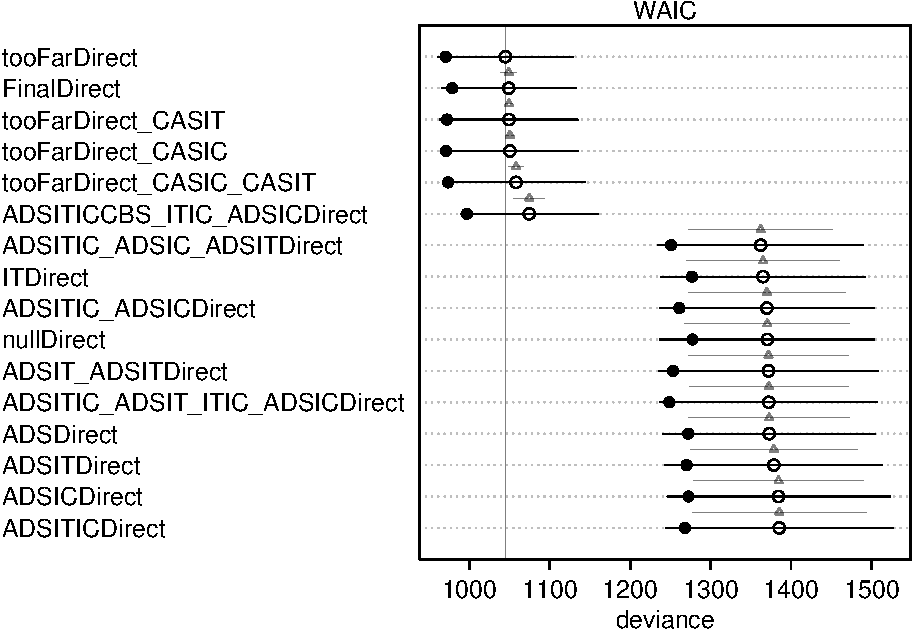
\includegraphics[width=1\linewidth]{bayesianReport3_files/figure-latex/comparisonDirectModels-1} \end{center}
\normalsize

Let's build a Hamiltonian Monte Carlo with the same formula:

\vspace{1mm}
\footnotesize

\begin{Shaded}
\begin{Highlighting}[]
\CommentTok{\# tooFarDirectHMC \textless{}{-} ulam(}
\CommentTok{\#   alist(}
\CommentTok{\#     AdiffS \textasciitilde{} dnorm( mu, sigma ),}
\CommentTok{\#     mu \textless{}{-} a + bADS[groupID] * ADS +  bIT[groupID] + bIC[groupID] * IC + }
\CommentTok{\#       bADSIC * ADS * IC+ bCBS[groupID] *CBS + bCBSIC * CBS * IC + bCAS * CAS, }
\CommentTok{\#     a \textasciitilde{} dnorm (0,0.3),}
\CommentTok{\#     bADS[groupID] \textasciitilde{} dnorm(0,.3),}
\CommentTok{\#     bADSIC \textasciitilde{} dnorm(0,.3),}
\CommentTok{\#     bCAS \textasciitilde{} dnorm(0,0.3),}
\CommentTok{\#     bCBS[groupID] \textasciitilde{} dnorm(0,.3),}
\CommentTok{\#     bIT[groupID] \textasciitilde{} dnorm(0,.3),}
\CommentTok{\#     bIC[groupID] \textasciitilde{} dnorm(0,.3),}
\CommentTok{\#     bCBSIC \textasciitilde{} dnorm(0, .3),}
\CommentTok{\#     sigma  \textasciitilde{} dexp(1)}
\CommentTok{\#   ), }
\CommentTok{\#   data = summaries}
\CommentTok{\# )}


\CommentTok{\#saveRDS(tooFarDirectHMC, file = "models/tooFarDirectHMC.rds")}

\NormalTok{tooFarDirectHMC }\OtherTok{\textless{}{-}} \FunctionTok{readRDS}\NormalTok{(}\AttributeTok{file =} \StringTok{"models/tooFarDirectHMC.rds"}\NormalTok{)}
\end{Highlighting}
\end{Shaded}

\normalsize

For a big picture, let's look at predicted direct effect by group and
user activity profile.

\vspace{1mm}
\footnotesize

\begin{Shaded}
\begin{Highlighting}[]
\NormalTok{visGroupDirect }\OtherTok{\textless{}{-}} \ControlFlowTok{function}\NormalTok{ (model, ADS, CBS, CAS, }\AttributeTok{xmin =}\DecValTok{2}\NormalTok{, }\AttributeTok{ymax =} \SpecialCharTok{{-}}\DecValTok{3}\NormalTok{)}
\NormalTok{\{}
\NormalTok{  groupID }\OtherTok{\textless{}{-}} \DecValTok{1}\SpecialCharTok{:}\DecValTok{3}
\NormalTok{  IC }\OtherTok{\textless{}{-}} \DecValTok{5} 
\NormalTok{  data }\OtherTok{\textless{}{-}} \FunctionTok{expand.grid}\NormalTok{(}\AttributeTok{ADS =}\NormalTok{ ADS,}\AttributeTok{groupID =}\NormalTok{ groupID, }\AttributeTok{CBS =}\NormalTok{ CBS, }\AttributeTok{CAS =}\NormalTok{ CAS, }\AttributeTok{IC =}\NormalTok{  IC)}
\NormalTok{  posterior }\OtherTok{\textless{}{-}} \FunctionTok{extract.samples}\NormalTok{(model, }\AttributeTok{n =} \FloatTok{1e5}\NormalTok{)}
\NormalTok{  mu }\OtherTok{\textless{}{-}} \FunctionTok{link}\NormalTok{( model, }\AttributeTok{data=}\NormalTok{data ) }
  \FunctionTok{colnames}\NormalTok{(mu) }\OtherTok{\textless{}{-}} \FunctionTok{levels}\NormalTok{(summaries}\SpecialCharTok{$}\NormalTok{group)}
\NormalTok{  muLong }\OtherTok{\textless{}{-}} \FunctionTok{melt}\NormalTok{(mu)}
  \FunctionTok{colnames}\NormalTok{(muLong) }\OtherTok{\textless{}{-}} \FunctionTok{c}\NormalTok{(}\StringTok{"id"}\NormalTok{, }\StringTok{"group"}\NormalTok{, }\StringTok{"AdiffS"}\NormalTok{)}
\NormalTok{  means }\OtherTok{\textless{}{-}}  \FunctionTok{round}\NormalTok{(}\FunctionTok{apply}\NormalTok{(mu , }\DecValTok{2}\NormalTok{ , mean ), }\DecValTok{2}\NormalTok{)}
\NormalTok{  mu\_HPDI }\OtherTok{\textless{}{-}} \FunctionTok{round}\NormalTok{(}\FunctionTok{apply}\NormalTok{( mu , }\DecValTok{2}\NormalTok{ , HPDI ),}\DecValTok{2}\NormalTok{)}
\NormalTok{  means }\OtherTok{\textless{}{-}} \FunctionTok{as.data.frame}\NormalTok{(means)}
\NormalTok{  means}\SpecialCharTok{$}\NormalTok{group }\OtherTok{\textless{}{-}} \FunctionTok{rownames}\NormalTok{(means)}
  \FunctionTok{rownames}\NormalTok{(means) }\OtherTok{\textless{}{-}} \ConstantTok{NULL}
\NormalTok{  meansDisp }\OtherTok{\textless{}{-}} \FunctionTok{cbind}\NormalTok{(means,}\FunctionTok{t}\NormalTok{(}\FunctionTok{as.data.frame}\NormalTok{(mu\_HPDI)))}
\NormalTok{  meansDisp }\OtherTok{\textless{}{-}}\NormalTok{ meansDisp[,}\FunctionTok{c}\NormalTok{(}\DecValTok{1}\NormalTok{,}\DecValTok{3}\NormalTok{,}\DecValTok{4}\NormalTok{)]}
  
\NormalTok{  plot }\OtherTok{\textless{}{-}} \FunctionTok{ggplot}\NormalTok{(muLong)}\SpecialCharTok{+}\FunctionTok{geom\_violin}\NormalTok{(}\FunctionTok{aes}\NormalTok{(}\AttributeTok{x =}\NormalTok{ group, }\AttributeTok{y =}\NormalTok{ AdiffS), }\AttributeTok{alpha =} \FloatTok{0.2}\NormalTok{)}\SpecialCharTok{+}
    \FunctionTok{xlab}\NormalTok{(}\StringTok{""}\NormalTok{)}\SpecialCharTok{+}
    \FunctionTok{labs}\NormalTok{(}\AttributeTok{title =} \FunctionTok{paste}\NormalTok{(}\StringTok{"ADS="}\NormalTok{, ADS, }\StringTok{", CBS="}\NormalTok{,  CBS, }\StringTok{", CAS="}\NormalTok{, CAS,  }\AttributeTok{sep =} \StringTok{""}\NormalTok{))}\SpecialCharTok{+}
    \FunctionTok{theme\_tufte}\NormalTok{()}\SpecialCharTok{+}\FunctionTok{ylim}\NormalTok{(}\FunctionTok{c}\NormalTok{(}\SpecialCharTok{{-}}\DecValTok{4}\NormalTok{,}\DecValTok{4}\NormalTok{))}
  \CommentTok{\#+   annotation\_custom(tableGrob(meansDisp), xmin=xmin,  ymax=ymax)}
  \FunctionTok{return}\NormalTok{(plot)}
\NormalTok{\}}



\NormalTok{visGroupDirect2\_2\_2 }\OtherTok{\textless{}{-}}  \FunctionTok{visGroupDirect}\NormalTok{(}\AttributeTok{model =}\NormalTok{ tooFarDirectHMC, }\AttributeTok{ADS =} \DecValTok{2}\NormalTok{,}\AttributeTok{CBS =} \SpecialCharTok{{-}}\DecValTok{2}\NormalTok{, }\AttributeTok{CAS =} \SpecialCharTok{{-}}\DecValTok{2}\NormalTok{)}
\NormalTok{visGroupDirect200 }\OtherTok{\textless{}{-}}  \FunctionTok{visGroupDirect}\NormalTok{(}\AttributeTok{model =}\NormalTok{ tooFarDirectHMC, }\AttributeTok{ADS =} \DecValTok{2}\NormalTok{,}\AttributeTok{CBS =} \DecValTok{0}\NormalTok{, }\AttributeTok{CAS =} \DecValTok{0}\NormalTok{)}
\NormalTok{visGroupDirect222 }\OtherTok{\textless{}{-}} \FunctionTok{visGroupDirect}\NormalTok{(}\AttributeTok{model =}\NormalTok{ tooFarDirectHMC, }\AttributeTok{ADS =} \DecValTok{2}\NormalTok{,}\AttributeTok{CBS =} \DecValTok{2}\NormalTok{, }\AttributeTok{CAS =} \DecValTok{2}\NormalTok{)}

\NormalTok{visGroupDirect0\_2\_2 }\OtherTok{\textless{}{-}}  \FunctionTok{visGroupDirect}\NormalTok{(}\AttributeTok{model =}\NormalTok{ tooFarDirectHMC, }\AttributeTok{ADS =} \DecValTok{0}\NormalTok{,}\AttributeTok{CBS =} \SpecialCharTok{{-}}\DecValTok{2}\NormalTok{, }\AttributeTok{CAS =} \SpecialCharTok{{-}}\DecValTok{2}\NormalTok{)}
\NormalTok{visGroupDirect000 }\OtherTok{\textless{}{-}}  \FunctionTok{visGroupDirect}\NormalTok{(}\AttributeTok{model =}\NormalTok{ tooFarDirectHMC, }\AttributeTok{ADS =} \DecValTok{0}\NormalTok{,}\AttributeTok{CBS =} \DecValTok{0}\NormalTok{, }\AttributeTok{CAS =} \DecValTok{0}\NormalTok{)}
\NormalTok{visGroupDirect022 }\OtherTok{\textless{}{-}} \FunctionTok{visGroupDirect}\NormalTok{(}\AttributeTok{model =}\NormalTok{ tooFarDirectHMC, }\AttributeTok{ADS =} \DecValTok{0}\NormalTok{,}\AttributeTok{CBS =} \DecValTok{2}\NormalTok{, }\AttributeTok{CAS =} \DecValTok{2}\NormalTok{)}


\NormalTok{visGroupDirect\_2\_2\_2 }\OtherTok{\textless{}{-}}  \FunctionTok{visGroupDirect}\NormalTok{(}\AttributeTok{model =}\NormalTok{ tooFarDirectHMC, }\AttributeTok{ADS =} \SpecialCharTok{{-}}\DecValTok{2}\NormalTok{,}\AttributeTok{CBS =} \SpecialCharTok{{-}}\DecValTok{2}\NormalTok{, }\AttributeTok{CAS =} \SpecialCharTok{{-}}\DecValTok{2}\NormalTok{)}
\NormalTok{visGroupDirect\_200 }\OtherTok{\textless{}{-}}  \FunctionTok{visGroupDirect}\NormalTok{(}\AttributeTok{model =}\NormalTok{ tooFarDirectHMC, }\AttributeTok{ADS =} \SpecialCharTok{{-}}\DecValTok{2}\NormalTok{,}\AttributeTok{CBS =} \DecValTok{0}\NormalTok{, }\AttributeTok{CAS =} \DecValTok{0}\NormalTok{)}
\NormalTok{visGroupDirect\_222 }\OtherTok{\textless{}{-}} \FunctionTok{visGroupDirect}\NormalTok{(}\AttributeTok{model =}\NormalTok{ tooFarDirectHMC, }\AttributeTok{ADS =} \SpecialCharTok{{-}}\DecValTok{2}\NormalTok{,}\AttributeTok{CBS =} \DecValTok{2}\NormalTok{, }\AttributeTok{CAS =} \DecValTok{2}\NormalTok{)}


\NormalTok{visGroupDirectJoint }\OtherTok{\textless{}{-}} \FunctionTok{ggarrange}\NormalTok{(visGroupDirect2\_2\_2}\SpecialCharTok{+}\NormalTok{removeX }\SpecialCharTok{+}\FunctionTok{ylab}\NormalTok{(}\StringTok{"ADS = 2"}\NormalTok{)}\SpecialCharTok{+}\FunctionTok{ggtitle}\NormalTok{(}\StringTok{"CBS = CAS = {-}2"}\NormalTok{),}
\NormalTok{                                 visGroupDirect200}\SpecialCharTok{+}\NormalTok{removeX}\SpecialCharTok{+}\NormalTok{removeY}\SpecialCharTok{+} \FunctionTok{ggtitle}\NormalTok{(}\StringTok{"CBS = CAS = 0"}\NormalTok{),}
\NormalTok{                                 visGroupDirect222}\SpecialCharTok{+}\NormalTok{removeX}\SpecialCharTok{+}\NormalTok{removeY}\SpecialCharTok{+} \FunctionTok{ggtitle}\NormalTok{(}\StringTok{"CBS = CAS = 2"}\NormalTok{) ,}
\NormalTok{                        visGroupDirect0\_2\_2}\SpecialCharTok{+}\NormalTok{removeX }\SpecialCharTok{+} \FunctionTok{ggtitle}\NormalTok{(}\StringTok{""}\NormalTok{)}\SpecialCharTok{+}\FunctionTok{ylab}\NormalTok{(}\StringTok{"ADS = 0"}\NormalTok{),}
\NormalTok{                                visGroupDirect000}\SpecialCharTok{+}\NormalTok{removeX}\SpecialCharTok{+}\NormalTok{removeY}\SpecialCharTok{+} \FunctionTok{ggtitle}\NormalTok{(}\StringTok{""}\NormalTok{),}
\NormalTok{                                visGroupDirect022}\SpecialCharTok{+}\NormalTok{removeX}\SpecialCharTok{+}\NormalTok{removeY}\SpecialCharTok{+} \FunctionTok{ggtitle}\NormalTok{(}\StringTok{""}\NormalTok{),}
\NormalTok{                        visGroupDirect\_2\_2\_2}\SpecialCharTok{+}\NormalTok{removeX}\SpecialCharTok{+}\FunctionTok{ylab}\NormalTok{(}\StringTok{"ADS = {-}2"}\NormalTok{)}\SpecialCharTok{+} \FunctionTok{ggtitle}\NormalTok{(}\StringTok{""}\NormalTok{),}
\NormalTok{                                  visGroupDirect\_200}\SpecialCharTok{+}\NormalTok{removeX}\SpecialCharTok{+}\NormalTok{removeY}\SpecialCharTok{+} \FunctionTok{ggtitle}\NormalTok{(}\StringTok{""}\NormalTok{),}
\NormalTok{                        visGroupDirect\_222}\SpecialCharTok{+}\NormalTok{removeX}\SpecialCharTok{+}\NormalTok{removeY}\SpecialCharTok{+} \FunctionTok{ggtitle}\NormalTok{(}\StringTok{""}\NormalTok{)}
\NormalTok{                                 ,}\AttributeTok{ncol =}\DecValTok{3}\NormalTok{, }\AttributeTok{nrow =} \DecValTok{3}\NormalTok{)}
                                  
      


\NormalTok{visGroupDirectJoint2 }\OtherTok{\textless{}{-}} \FunctionTok{annotate\_figure}\NormalTok{(visGroupDirectJoint, }
                                  \AttributeTok{top =} \FunctionTok{text\_grob}\NormalTok{(}\StringTok{"(range restricted to ({-}4,4), IC at the rounded mean = 5)"}\NormalTok{,}
                                                  \AttributeTok{size =} \DecValTok{10}\NormalTok{))}
\NormalTok{visGroupJoint3 }\OtherTok{\textless{}{-}} \FunctionTok{annotate\_figure}\NormalTok{(visGroupDirectJoint2, }
                                  \AttributeTok{top =} \FunctionTok{text\_grob}\NormalTok{(}\StringTok{"Predicted direct effect of treatment group by activity profile (standardized)"}\NormalTok{,}
                                                  \AttributeTok{size =} \DecValTok{12}\NormalTok{))}

\NormalTok{visGroupJoint3}
\end{Highlighting}
\end{Shaded}

\begin{center}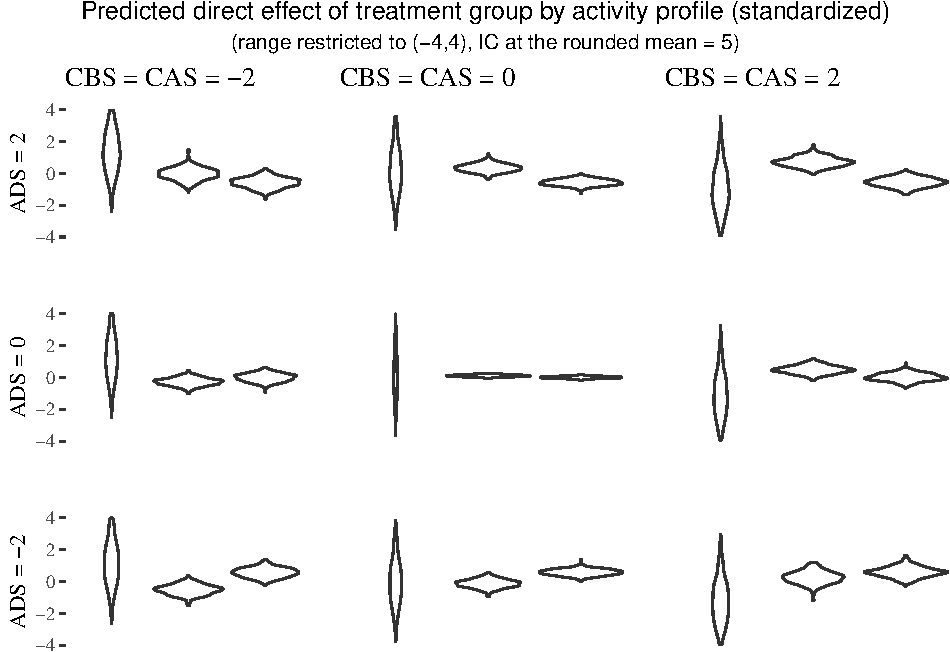
\includegraphics[width=1\linewidth]{bayesianReport3_files/figure-latex/unnamed-chunk-17-1} \end{center}
\normalsize

Now, predicted direct effect of five interventions vs.~\textsf{CBS}, for
three user activity profiles.

\vspace{1mm}
\footnotesize

\begin{Shaded}
\begin{Highlighting}[]
\NormalTok{visContrastsCBSDirect }\OtherTok{\textless{}{-}} \ControlFlowTok{function}\NormalTok{(}\AttributeTok{model =}\NormalTok{ FinalHMC, }\AttributeTok{ADS =}\NormalTok{ ADS , }\AttributeTok{CAS=}\NormalTok{ CAS, }\AttributeTok{IC =}  \DecValTok{5}\NormalTok{,}
                            \AttributeTok{CBS =} \FunctionTok{seq}\NormalTok{(}\SpecialCharTok{{-}}\DecValTok{3}\NormalTok{,}\DecValTok{3}\NormalTok{,}\AttributeTok{by  =} \FloatTok{0.1}\NormalTok{))\{}
\NormalTok{  groupID }\OtherTok{\textless{}{-}} \DecValTok{1}\SpecialCharTok{:}\DecValTok{3}
\NormalTok{  data }\OtherTok{\textless{}{-}} \FunctionTok{expand.grid}\NormalTok{(ADS, groupID, CAS, IC , CBS)}
  \FunctionTok{colnames}\NormalTok{(data) }\OtherTok{\textless{}{-}} \FunctionTok{c}\NormalTok{(}\StringTok{"ADS"}\NormalTok{, }\StringTok{"groupID"}\NormalTok{, }\StringTok{"CAS"}\NormalTok{, }\StringTok{"IC"}\NormalTok{, }\StringTok{"CBS"}\NormalTok{)}
\NormalTok{  posterior }\OtherTok{\textless{}{-}} \FunctionTok{extract.samples}\NormalTok{(model, }\AttributeTok{n =} \FloatTok{1e5}\NormalTok{)}
  \FunctionTok{link}\NormalTok{( model, }\AttributeTok{data=}\NormalTok{data ) }
\NormalTok{  mu }\OtherTok{\textless{}{-}} \FunctionTok{link}\NormalTok{( model, }\AttributeTok{data=}\NormalTok{data ) }
  
\NormalTok{  means }\OtherTok{\textless{}{-}}  \FunctionTok{round}\NormalTok{(}\FunctionTok{apply}\NormalTok{(mu , }\DecValTok{2}\NormalTok{ , mean ), }\DecValTok{4}\NormalTok{)}
  
\NormalTok{  HPDIs }\OtherTok{\textless{}{-}} \FunctionTok{round}\NormalTok{(}\FunctionTok{apply}\NormalTok{( mu , }\DecValTok{2}\NormalTok{ , HPDI ),}\DecValTok{4}\NormalTok{)}
\NormalTok{  visContrast }\OtherTok{\textless{}{-}} \FunctionTok{cbind}\NormalTok{(data,means,}\FunctionTok{t}\NormalTok{(}\FunctionTok{as.data.frame}\NormalTok{(HPDIs)))}
  
\NormalTok{  ones }\OtherTok{\textless{}{-}} \DecValTok{3} \SpecialCharTok{*}\NormalTok{ (}\DecValTok{1}\SpecialCharTok{:}\NormalTok{(}\FunctionTok{nrow}\NormalTok{(visContrast)}\SpecialCharTok{/}\DecValTok{3}\NormalTok{))}\SpecialCharTok{{-}}\DecValTok{2}
\NormalTok{  twos }\OtherTok{\textless{}{-}} \DecValTok{3} \SpecialCharTok{*}\NormalTok{ (}\DecValTok{1}\SpecialCharTok{:}\NormalTok{(}\FunctionTok{nrow}\NormalTok{(visContrast)}\SpecialCharTok{/}\DecValTok{3}\NormalTok{))}\SpecialCharTok{{-}}\DecValTok{1}
\NormalTok{  threes }\OtherTok{\textless{}{-}} \DecValTok{3} \SpecialCharTok{*}\NormalTok{ (}\DecValTok{1}\SpecialCharTok{:}\NormalTok{(}\FunctionTok{nrow}\NormalTok{(visContrast)}\SpecialCharTok{/}\DecValTok{3}\NormalTok{))}
  
  \FunctionTok{colnames}\NormalTok{(visContrast)[}\FunctionTok{c}\NormalTok{(}\DecValTok{7}\NormalTok{,}\DecValTok{8}\NormalTok{)] }\OtherTok{\textless{}{-}} \FunctionTok{c}\NormalTok{(}\StringTok{"low"}\NormalTok{, }\StringTok{"high"}\NormalTok{)}
  
\NormalTok{  contrast }\OtherTok{\textless{}{-}} \FunctionTok{numeric}\NormalTok{(}\FunctionTok{nrow}\NormalTok{(visContrast))}
\NormalTok{  cLow }\OtherTok{\textless{}{-}} \FunctionTok{numeric}\NormalTok{(}\FunctionTok{nrow}\NormalTok{(visContrast))}
\NormalTok{  cHigh }\OtherTok{\textless{}{-}} \FunctionTok{numeric}\NormalTok{(}\FunctionTok{nrow}\NormalTok{(visContrast))}
  \ControlFlowTok{for}\NormalTok{(i }\ControlFlowTok{in}\NormalTok{ threes)\{}
\NormalTok{    contrast[i] }\OtherTok{\textless{}{-}}\NormalTok{ visContrast}\SpecialCharTok{$}\NormalTok{means[i] }\SpecialCharTok{{-}}\NormalTok{ visContrast}\SpecialCharTok{$}\NormalTok{means[i}\DecValTok{{-}2}\NormalTok{]  }
\NormalTok{  \}}
  \ControlFlowTok{for}\NormalTok{(i }\ControlFlowTok{in}\NormalTok{ twos)\{}
\NormalTok{    contrast[i] }\OtherTok{\textless{}{-}}\NormalTok{ visContrast}\SpecialCharTok{$}\NormalTok{means[i] }\SpecialCharTok{{-}}\NormalTok{ visContrast}\SpecialCharTok{$}\NormalTok{means[i}\DecValTok{{-}1}\NormalTok{]  }
\NormalTok{  \}}
\NormalTok{  visContrast}\SpecialCharTok{$}\NormalTok{contrast }\OtherTok{\textless{}{-}}\NormalTok{ contrast}
\NormalTok{  visContrast}\SpecialCharTok{$}\NormalTok{shift }\OtherTok{\textless{}{-}}\NormalTok{  visContrast}\SpecialCharTok{$}\NormalTok{contrast }\SpecialCharTok{{-}}\NormalTok{ visContrast}\SpecialCharTok{$}\NormalTok{means}
  \ControlFlowTok{for}\NormalTok{(i }\ControlFlowTok{in}\NormalTok{ ones)\{}
\NormalTok{    visContrast}\SpecialCharTok{$}\NormalTok{shift[i] }\OtherTok{\textless{}{-}} \DecValTok{0}
\NormalTok{  \}}
\NormalTok{  visContrast}\SpecialCharTok{$}\NormalTok{cLow }\OtherTok{\textless{}{-}}\NormalTok{ visContrast}\SpecialCharTok{$}\NormalTok{low }\SpecialCharTok{+}\NormalTok{ visContrast}\SpecialCharTok{$}\NormalTok{shift}
\NormalTok{  visContrast}\SpecialCharTok{$}\NormalTok{cHigh }\OtherTok{\textless{}{-}}\NormalTok{ visContrast}\SpecialCharTok{$}\NormalTok{high }\SpecialCharTok{+}\NormalTok{ visContrast}\SpecialCharTok{$}\NormalTok{shift}
  
\NormalTok{  visContrast}\SpecialCharTok{$}\NormalTok{group }\OtherTok{=} \FunctionTok{rep}\NormalTok{(}\FunctionTok{c}\NormalTok{(}\StringTok{"control"}\NormalTok{, }\StringTok{"empathy"}\NormalTok{, }\StringTok{"normative"}\NormalTok{), }
                          \FunctionTok{nrow}\NormalTok{(visContrast)}\SpecialCharTok{/}\DecValTok{3}\NormalTok{)}
  
\NormalTok{  visContrastTreatment }\OtherTok{\textless{}{-}}\NormalTok{ visContrast[groupID }\SpecialCharTok{!=}\DecValTok{1}\NormalTok{,]}
  
  \FunctionTok{return}\NormalTok{(}\FunctionTok{ggplot}\NormalTok{(visContrastTreatment, }\FunctionTok{aes}\NormalTok{(}\AttributeTok{x =}\NormalTok{ CBS, }\AttributeTok{y =}\NormalTok{ contrast, }\AttributeTok{fill =}\NormalTok{ group ))}\SpecialCharTok{+}
           \FunctionTok{geom\_line}\NormalTok{(}\AttributeTok{se =} \ConstantTok{FALSE}\NormalTok{)}\SpecialCharTok{+}
           \FunctionTok{geom\_ribbon}\NormalTok{(}\AttributeTok{mapping =} 
                         \FunctionTok{aes}\NormalTok{(}\AttributeTok{ymin =}\NormalTok{ cLow, }\AttributeTok{ymax =}\NormalTok{ cHigh),  }
                       \AttributeTok{alpha =}\NormalTok{ .}\DecValTok{3}\NormalTok{)}\SpecialCharTok{+}
           \FunctionTok{theme\_tufte}\NormalTok{()}\SpecialCharTok{+}\FunctionTok{ylim}\NormalTok{(}\FunctionTok{c}\NormalTok{(}\SpecialCharTok{{-}}\FloatTok{3.5}\NormalTok{,}\FloatTok{3.5}\NormalTok{)))}
\NormalTok{\}}

\NormalTok{visContrastDirect }\OtherTok{\textless{}{-}}  \FunctionTok{ggarrange}\NormalTok{(}\FunctionTok{visContrastsCBSDirect}\NormalTok{(}\AttributeTok{model =}\NormalTok{ tooFarDirect,}\AttributeTok{ADS =} \SpecialCharTok{{-}}\DecValTok{2}\NormalTok{, }\AttributeTok{CAS =} \SpecialCharTok{{-}}\DecValTok{2}\NormalTok{, }\AttributeTok{IC =} \DecValTok{5}\NormalTok{)}\SpecialCharTok{+}\FunctionTok{ggtitle}\NormalTok{(}\StringTok{"ADS = CAS = {-}2"}\NormalTok{)}\SpecialCharTok{+} \FunctionTok{scale\_fill\_discrete}\NormalTok{(}\AttributeTok{guide=}\ConstantTok{FALSE}\NormalTok{),}
          \FunctionTok{visContrastsCBSDirect}\NormalTok{(}\AttributeTok{model =}\NormalTok{ tooFarDirect,}\AttributeTok{ADS =} \DecValTok{0}\NormalTok{, }\AttributeTok{CAS =} \DecValTok{0}\NormalTok{, }\AttributeTok{IC =} \DecValTok{5}\NormalTok{) }\SpecialCharTok{+}\FunctionTok{ggtitle}\NormalTok{(}\StringTok{"ADS = CAS = 0"}\NormalTok{)}\SpecialCharTok{+} \FunctionTok{scale\_fill\_discrete}\NormalTok{(}\AttributeTok{guide=}\ConstantTok{FALSE}\NormalTok{)}\SpecialCharTok{+}\NormalTok{removeY,}
          \FunctionTok{visContrastsCBSDirect}\NormalTok{(}\AttributeTok{model =}\NormalTok{ tooFarDirect,}\AttributeTok{ADS =} \DecValTok{2}\NormalTok{, }\AttributeTok{CAS =} \DecValTok{2}\NormalTok{, }\AttributeTok{IC =} \DecValTok{5}\NormalTok{) }\SpecialCharTok{+}\FunctionTok{ggtitle}\NormalTok{(}\StringTok{"ADS = CAS = 2"}\NormalTok{)}\SpecialCharTok{+} \FunctionTok{scale\_fill\_discrete}\NormalTok{(}\AttributeTok{guide=}\ConstantTok{FALSE}\NormalTok{)}\SpecialCharTok{+}\NormalTok{removeY}
\NormalTok{          ,}\AttributeTok{ncol =}\DecValTok{3}\NormalTok{)}
\end{Highlighting}
\end{Shaded}

\begin{verbatim}
## Warning: Ignoring unknown parameters: se

## Warning: Ignoring unknown parameters: se

## Warning: Ignoring unknown parameters: se
\end{verbatim}

\begin{verbatim}
## Warning: It is deprecated to specify `guide = FALSE` to remove a guide. Please
## use `guide = "none"` instead.

## Warning: It is deprecated to specify `guide = FALSE` to remove a guide. Please
## use `guide = "none"` instead.

## Warning: It is deprecated to specify `guide = FALSE` to remove a guide. Please
## use `guide = "none"` instead.
\end{verbatim}

\begin{Shaded}
\begin{Highlighting}[]
\NormalTok{visContrastDirect2 }\OtherTok{\textless{}{-}} \FunctionTok{annotate\_figure}\NormalTok{(visContrastDirect, }
                                        \AttributeTok{top =} \FunctionTok{text\_grob}\NormalTok{(}\StringTok{"(range restricted to ({-}3.5,3.5), IC at the rounded mean = 5)"}\NormalTok{,}
                                                        \AttributeTok{size =} \DecValTok{10}\NormalTok{))}
\NormalTok{visContrastDirect3 }\OtherTok{\textless{}{-}} \FunctionTok{annotate\_figure}\NormalTok{(visContrastDirect2, }
                                        \AttributeTok{top =} \FunctionTok{text\_grob}\NormalTok{(}\StringTok{"Predicted direct effect distance from the control group mean vs. CBS  (standardized)"}\NormalTok{,}
                                                        \AttributeTok{size =} \DecValTok{12}\NormalTok{))}

\NormalTok{visContrastDirect3}
\end{Highlighting}
\end{Shaded}

\begin{center}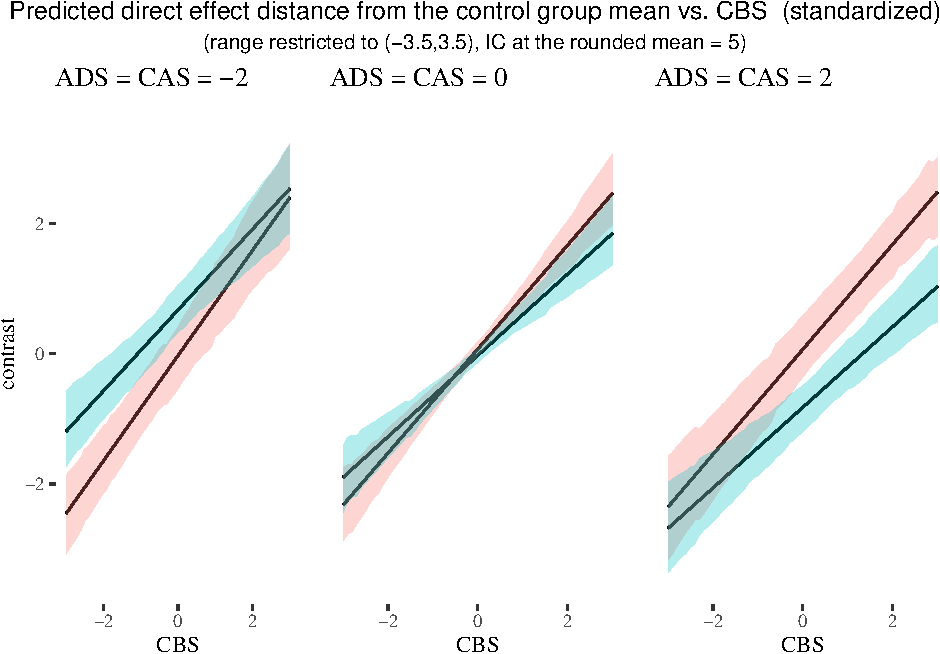
\includegraphics[width=1\linewidth]{bayesianReport3_files/figure-latex/unnamed-chunk-18-1} \end{center}
\normalsize

Now contrasts against \textsf{ADS}, for three user profiles:

\vspace{1mm}
\footnotesize

\begin{Shaded}
\begin{Highlighting}[]
\NormalTok{visContrastsADSDirect }\OtherTok{\textless{}{-}} \ControlFlowTok{function}\NormalTok{(}\AttributeTok{model =}\NormalTok{ FinalHMC, }\AttributeTok{CBS =}\NormalTok{ CBS , }\AttributeTok{CAS =}\NormalTok{ CAS, }\AttributeTok{IC =}  \DecValTok{5}\NormalTok{, }
                            \AttributeTok{ADS =} \FunctionTok{seq}\NormalTok{(}\SpecialCharTok{{-}}\DecValTok{3}\NormalTok{,}\DecValTok{3}\NormalTok{,}\AttributeTok{by  =} \FloatTok{0.1}\NormalTok{))}
\NormalTok{\{}
\NormalTok{  data }\OtherTok{\textless{}{-}} \FunctionTok{expand.grid}\NormalTok{(CBS, groupID, CAS, IC , ADS)}
  \FunctionTok{colnames}\NormalTok{(data) }\OtherTok{\textless{}{-}} \FunctionTok{c}\NormalTok{(}\StringTok{"CBS"}\NormalTok{, }\StringTok{"groupID"}\NormalTok{, }\StringTok{"CAS"}\NormalTok{, }\StringTok{"IC"}\NormalTok{, }\StringTok{"ADS"}\NormalTok{)}
\NormalTok{  posterior }\OtherTok{\textless{}{-}} \FunctionTok{extract.samples}\NormalTok{(model, }\AttributeTok{n =} \FloatTok{1e5}\NormalTok{)}
\NormalTok{  mu }\OtherTok{\textless{}{-}} \FunctionTok{link}\NormalTok{( model, }\AttributeTok{data=}\NormalTok{data ) }
\NormalTok{  means }\OtherTok{\textless{}{-}}  \FunctionTok{round}\NormalTok{(}\FunctionTok{apply}\NormalTok{(mu , }\DecValTok{2}\NormalTok{ , mean ), }\DecValTok{4}\NormalTok{)}
\NormalTok{  HPDIs }\OtherTok{\textless{}{-}} \FunctionTok{round}\NormalTok{(}\FunctionTok{apply}\NormalTok{( mu , }\DecValTok{2}\NormalTok{ , HPDI ),}\DecValTok{4}\NormalTok{)}
\NormalTok{  visContrastADS }\OtherTok{\textless{}{-}} \FunctionTok{cbind}\NormalTok{(data,means,}\FunctionTok{t}\NormalTok{(}\FunctionTok{as.data.frame}\NormalTok{(HPDIs)))}
  
  
\NormalTok{  ones }\OtherTok{\textless{}{-}} \DecValTok{3} \SpecialCharTok{*}\NormalTok{ (}\DecValTok{1}\SpecialCharTok{:}\NormalTok{(}\FunctionTok{nrow}\NormalTok{(visContrastADS)}\SpecialCharTok{/}\DecValTok{3}\NormalTok{))}\SpecialCharTok{{-}}\DecValTok{2}
\NormalTok{  twos }\OtherTok{\textless{}{-}} \DecValTok{3} \SpecialCharTok{*}\NormalTok{ (}\DecValTok{1}\SpecialCharTok{:}\NormalTok{(}\FunctionTok{nrow}\NormalTok{(visContrastADS)}\SpecialCharTok{/}\DecValTok{3}\NormalTok{))}\SpecialCharTok{{-}}\DecValTok{1}
\NormalTok{  threes }\OtherTok{\textless{}{-}} \DecValTok{3} \SpecialCharTok{*}\NormalTok{ (}\DecValTok{1}\SpecialCharTok{:}\NormalTok{(}\FunctionTok{nrow}\NormalTok{(visContrastADS)}\SpecialCharTok{/}\DecValTok{3}\NormalTok{))}
  
  \FunctionTok{colnames}\NormalTok{(visContrastADS)[}\FunctionTok{c}\NormalTok{(}\DecValTok{7}\NormalTok{,}\DecValTok{8}\NormalTok{)] }\OtherTok{\textless{}{-}} \FunctionTok{c}\NormalTok{(}\StringTok{"low"}\NormalTok{, }\StringTok{"high"}\NormalTok{)}
\NormalTok{  contrastADS }\OtherTok{\textless{}{-}} \FunctionTok{numeric}\NormalTok{(}\FunctionTok{nrow}\NormalTok{(visContrastADS))}
  \ControlFlowTok{for}\NormalTok{(i }\ControlFlowTok{in}\NormalTok{ threes)\{}
\NormalTok{    contrastADS[i] }\OtherTok{\textless{}{-}}\NormalTok{ visContrastADS}\SpecialCharTok{$}\NormalTok{means[i] }\SpecialCharTok{{-}}\NormalTok{ visContrastADS}\SpecialCharTok{$}\NormalTok{means[i}\DecValTok{{-}2}\NormalTok{]  }
\NormalTok{  \}}
  \ControlFlowTok{for}\NormalTok{(i }\ControlFlowTok{in}\NormalTok{ twos)\{}
\NormalTok{    contrastADS[i] }\OtherTok{\textless{}{-}}\NormalTok{ visContrastADS}\SpecialCharTok{$}\NormalTok{means[i] }\SpecialCharTok{{-}}\NormalTok{ visContrastADS}\SpecialCharTok{$}\NormalTok{means[i}\DecValTok{{-}1}\NormalTok{]  }
\NormalTok{  \}}
\NormalTok{  visContrastADS}\SpecialCharTok{$}\NormalTok{contrast }\OtherTok{\textless{}{-}}\NormalTok{ contrastADS}
\NormalTok{  visContrastADS}\SpecialCharTok{$}\NormalTok{shift }\OtherTok{\textless{}{-}}\NormalTok{  visContrastADS}\SpecialCharTok{$}\NormalTok{contrast }\SpecialCharTok{{-}}\NormalTok{ visContrastADS}\SpecialCharTok{$}\NormalTok{means}
  \ControlFlowTok{for}\NormalTok{(i }\ControlFlowTok{in}\NormalTok{ ones)\{}
\NormalTok{    visContrastADS}\SpecialCharTok{$}\NormalTok{shift[i] }\OtherTok{\textless{}{-}} \DecValTok{0}
\NormalTok{  \}}
\NormalTok{  visContrastADS}\SpecialCharTok{$}\NormalTok{cLow }\OtherTok{\textless{}{-}}\NormalTok{ visContrastADS}\SpecialCharTok{$}\NormalTok{low }\SpecialCharTok{+}\NormalTok{ visContrastADS}\SpecialCharTok{$}\NormalTok{shift}
\NormalTok{  visContrastADS}\SpecialCharTok{$}\NormalTok{cHigh }\OtherTok{\textless{}{-}}\NormalTok{ visContrastADS}\SpecialCharTok{$}\NormalTok{high }\SpecialCharTok{+}\NormalTok{ visContrastADS}\SpecialCharTok{$}\NormalTok{shift}
  
\NormalTok{  visContrastADS}\SpecialCharTok{$}\NormalTok{group }\OtherTok{=} \FunctionTok{rep}\NormalTok{(}\FunctionTok{c}\NormalTok{(}\StringTok{"control"}\NormalTok{, }\StringTok{"empathy"}\NormalTok{, }\StringTok{"normative"}\NormalTok{), }
                             \FunctionTok{nrow}\NormalTok{(visContrastADS)}\SpecialCharTok{/}\DecValTok{3}\NormalTok{)}
\NormalTok{  visContrastTreatmentADS }\OtherTok{\textless{}{-}}\NormalTok{ visContrastADS[groupID }\SpecialCharTok{!=}\DecValTok{1}\NormalTok{,]}
  
  \FunctionTok{return}\NormalTok{(}\FunctionTok{ggplot}\NormalTok{(visContrastTreatmentADS, }\FunctionTok{aes}\NormalTok{(}\AttributeTok{x =}\NormalTok{ ADS, }\AttributeTok{y =}\NormalTok{ contrast, }\AttributeTok{fill =}\NormalTok{ group ))}\SpecialCharTok{+}
           \FunctionTok{geom\_line}\NormalTok{(}\AttributeTok{se =} \ConstantTok{FALSE}\NormalTok{) }\SpecialCharTok{+}
           \FunctionTok{geom\_ribbon}\NormalTok{(}\AttributeTok{mapping =} \FunctionTok{aes}\NormalTok{(}\AttributeTok{ymin =}\NormalTok{ cLow, }\AttributeTok{ymax =}\NormalTok{ cHigh), }
                       \AttributeTok{alpha =}\NormalTok{ .}\DecValTok{3}\NormalTok{) }\SpecialCharTok{+}\FunctionTok{theme\_tufte}\NormalTok{())}
\NormalTok{\}}





\NormalTok{visContrastADSDirectJoint }\OtherTok{\textless{}{-}} \FunctionTok{ggarrange}\NormalTok{(}
  \FunctionTok{visContrastsADSDirect}\NormalTok{(tooFarDirect,}\AttributeTok{CBS =} \SpecialCharTok{{-}}\DecValTok{2}\NormalTok{, }\AttributeTok{CAS =} \SpecialCharTok{{-}}\DecValTok{2}\NormalTok{)}\SpecialCharTok{+}\FunctionTok{ggtitle}\NormalTok{(}\StringTok{"CBS = CAS = {-}2"}\NormalTok{)}\SpecialCharTok{+}\FunctionTok{ylim}\NormalTok{(}\FunctionTok{c}\NormalTok{(}\SpecialCharTok{{-}}\DecValTok{3}\NormalTok{,}\DecValTok{3}\NormalTok{))}\SpecialCharTok{+} \FunctionTok{scale\_fill\_discrete}\NormalTok{(}\AttributeTok{guide=}\ConstantTok{FALSE}\NormalTok{),}
  \FunctionTok{visContrastsADSDirect}\NormalTok{(tooFarDirect, }\AttributeTok{CBS =} \DecValTok{0}\NormalTok{, }\AttributeTok{CAS =} \DecValTok{0}\NormalTok{)}\SpecialCharTok{+}\FunctionTok{ggtitle}\NormalTok{(}\StringTok{"CBS = CAS = 0"}\NormalTok{)}\SpecialCharTok{+}\FunctionTok{ylim}\NormalTok{(}\FunctionTok{c}\NormalTok{(}\SpecialCharTok{{-}}\DecValTok{3}\NormalTok{,}\DecValTok{3}\NormalTok{))}\SpecialCharTok{+} \FunctionTok{scale\_fill\_discrete}\NormalTok{(}\AttributeTok{guide=}\ConstantTok{FALSE}\NormalTok{),}
  \FunctionTok{visContrastsADSDirect}\NormalTok{(tooFarDirect, }\AttributeTok{CBS =} \DecValTok{2}\NormalTok{, }\AttributeTok{CAS =} \DecValTok{2}\NormalTok{)}\SpecialCharTok{+}\FunctionTok{ggtitle}\NormalTok{(}\StringTok{"CBS = CAS = 2"}\NormalTok{)}\SpecialCharTok{+}\FunctionTok{ylim}\NormalTok{(}\FunctionTok{c}\NormalTok{(}\SpecialCharTok{{-}}\DecValTok{3}\NormalTok{,}\DecValTok{3}\NormalTok{))}\SpecialCharTok{+} \FunctionTok{scale\_fill\_discrete}\NormalTok{(}\AttributeTok{guide=}\ConstantTok{FALSE}\NormalTok{),}
  \AttributeTok{ncol =}\DecValTok{3}\NormalTok{)}
\end{Highlighting}
\end{Shaded}

\begin{verbatim}
## Warning: Ignoring unknown parameters: se

## Warning: Ignoring unknown parameters: se

## Warning: Ignoring unknown parameters: se
\end{verbatim}

\begin{verbatim}
## Warning: It is deprecated to specify `guide = FALSE` to remove a guide. Please
## use `guide = "none"` instead.

## Warning: It is deprecated to specify `guide = FALSE` to remove a guide. Please
## use `guide = "none"` instead.

## Warning: It is deprecated to specify `guide = FALSE` to remove a guide. Please
## use `guide = "none"` instead.
\end{verbatim}

\begin{Shaded}
\begin{Highlighting}[]
\NormalTok{visContrastADSDirectJoint2 }\OtherTok{\textless{}{-}} \FunctionTok{annotate\_figure}\NormalTok{(visContrastADSDirectJoint, }
                                        \AttributeTok{top =} \FunctionTok{text\_grob}\NormalTok{(}\StringTok{"(range restricted to ({-}3,3), IC at the rounded mean = 5)"}\NormalTok{,}
                                                        \AttributeTok{size =} \DecValTok{10}\NormalTok{))}
\NormalTok{visContrastADSDirectJoint3 }\OtherTok{\textless{}{-}} \FunctionTok{annotate\_figure}\NormalTok{(visContrastADSDirectJoint2, }
                                        \AttributeTok{top =} \FunctionTok{text\_grob}\NormalTok{(}\StringTok{"Predicted direct effect distance from the control group mean vs. ADS (standardized)"}\NormalTok{,}
                                                        \AttributeTok{size =} \DecValTok{12}\NormalTok{))}

\NormalTok{visContrastADSDirectJoint3}
\end{Highlighting}
\end{Shaded}

\begin{center}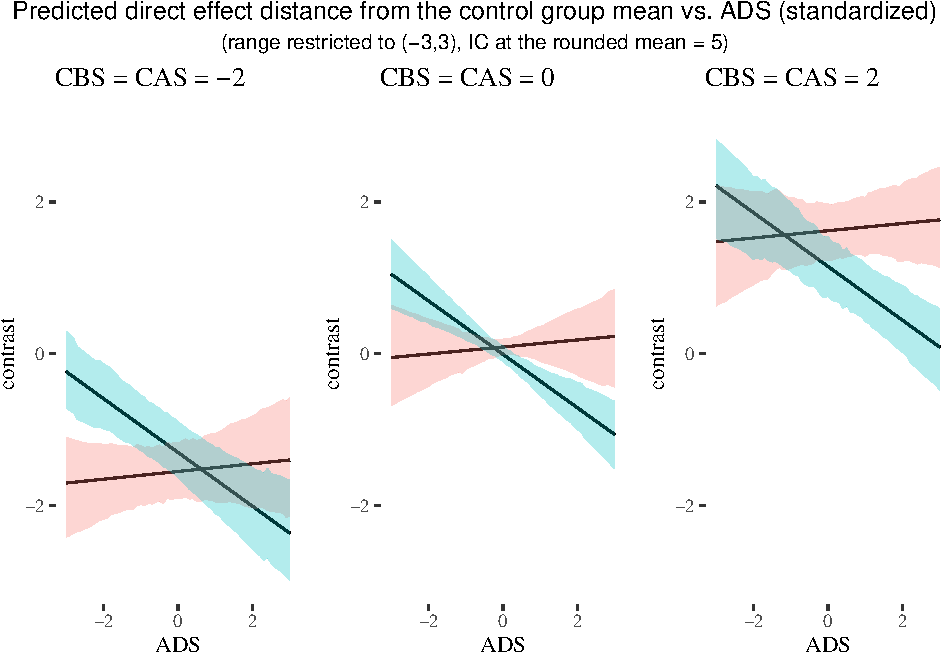
\includegraphics[width=1\linewidth]{bayesianReport3_files/figure-latex/unnamed-chunk-19-1} \end{center}
\normalsize

\hypertarget{references}{%
\section*{References}\label{references}}
\addcontentsline{toc}{section}{References}

\vspace{-3mm}

\end{document}
